% ***************************************************
% A Classic Thesis Style
% An Homage to The Elements of Typographic Style
%
% Copyright (C) 2012 Andr\'e Miede http://www.miede.de
%
% If you like the style then I would appreciate a postcard. My
% address can be found in the file ClassicThesis.pdf. A collection
% of the postcards I received so far is available online at 
% http://postcards.miede.de
%
% License:
% This program is free software; you can redistribute it and/or
% modify it under the terms of the GNU General Public License as
% published by the Free Software Foundation; either version 2 of
% the License, or (at your option) any later version.
%
% This program is distributed in the hope that it will be useful,
% but WITHOUT ANY WARRANTY; without even the implied warranty of
% MERCHANTABILITY or FITNESS FOR A PARTICULAR PURPOSE.  See the
% GNU General Public License for more details.
%
% You should have received a copy of the GNU General Public
% License along with this program; see the file COPYING.  If not,
% write to the Free Software Foundation, Inc., 59 Temple Place -
% Suite 330, Boston, MA 02111-1307, USA.
%
% ***************************************************************
% Note:
%    * You must not use "u etc. in strings/commands that will be spaced out (use \"u or real umlauts instead)
%    * New enumeration (small caps): \begin{aenumerate} \end{aenumerate}
%    * For margin notes: \marginpar or \graffito{}
%    * Do not use bold fonts in this style, it is designed around them
%    * Use tables as in the examples
%    * See classicthesis-preamble.sty for useful commands
% ****************************************************************
\documentclass[ twoside, 
			openright,
			% letterpaper a4paper
			titlepage, 
			numbers=noenddot,
			headinclude, %1headlines
            		footinclude=true, 
			cleardoublepage=empty,
			abstractoff, % <--- obsolete, remove (todo)
			BCOR=5mm,
			paper=a4, 
			fontsize=11pt, %11pt,
			]{scrreprt}

%*****************************************************************
% Note: Make all your adjustments in here
%*****************************************************************
\usepackage{mymacros}
%Theorems
\usepackage{amsthm,thmtools,thm-restate}
\newtheorem{assumption}{Assumption}
% \usepackage[backref, backend=biber]{biblatex}
\usepackage[backref,
		backend=bibtex,
            	maxbibnames=99,
            	natbib=true,
            	firstinits=false,
            	style=authoryear-comp,
            	sortcites=false,
            	doi=false,
            	url=false]{biblatex}           	
\bibliography{Bibliography}

% ****************************************************************
% classicthesis-config.tex 
% formerly known as loadpackages.sty, classicthesis-ldpkg.sty, and
% classicthesis-preamble.sty Use it at the beginning of your
% ClassicThesis.tex, or as a LaTeX Preamble in your
% ClassicThesis.{tex,lyx} with % ****************************************************************
% classicthesis-config.tex 
% formerly known as loadpackages.sty, classicthesis-ldpkg.sty, and
% classicthesis-preamble.sty Use it at the beginning of your
% ClassicThesis.tex, or as a LaTeX Preamble in your
% ClassicThesis.{tex,lyx} with % ****************************************************************
% classicthesis-config.tex 
% formerly known as loadpackages.sty, classicthesis-ldpkg.sty, and
% classicthesis-preamble.sty Use it at the beginning of your
% ClassicThesis.tex, or as a LaTeX Preamble in your
% ClassicThesis.{tex,lyx} with \input{classicthesis-config}
% ****************************************************************
% If you like the classicthesis, then I would appreciate a
% postcard. My address can be found in the file
% ClassicThesis.pdf. A collection of the postcards I received so
% far is available online at http://postcards.miede.de
% ****************************************************************

% ****************************************************************
% 1. Configure classicthesis for your needs here, e.g., remove
% "drafting" below in order to deactivate the time-stamp on the
% pages
% ****************************************************************
\PassOptionsToPackage{eulerchapternumbers,
					listings,
					%drafting,
				 	pdfspacing,
					floatperchapter,
					%linedheaders,
				 	subfig,
					beramono,
					eulermath,
					parts}{classicthesis}										

% ****************************************************************
% Triggers for this config
% **************************************************************** 
\usepackage{ifthen}
\newboolean{enable-backrefs} % enable backrefs in the bibliography
\setboolean{enable-backrefs}{false} % true false
% TODO backref is incompatible?
% ****************************************************************


% ****************************************************************
% 2. Personal data and user ad-hoc commands
% ****************************************************************
\newcommand{\myTitle}{Deterministic Policy Optimization:\xspace}
\newcommand{\mySubtitle}{an Approach to Safe Reinforcement Learning\xspace}
\newcommand{\myTitleIT}{Un modello per tesi di laurea magistrale al DEIB \xspace}
\newcommand{\myFirstAuthorName}{Pietro Melzi\xspace}
\newcommand{\myMatrFirstAuthor}{900217\xspace}
\newcommand{\mySecondAuthorName}{Emanuele Mason\xspace}
\newcommand{\myMatrSecondAuthor}{222222\xspace}
\newcommand{\mySupervisor}{Prof. Marcello Restelli\xspace} % relatore
\newcommand{\myOtherSupervisor}{Dott. Matteo Papini\xspace} % co relatori
\newcommand{\myOtherOtherSupervisor}{Prof. my ASP supervisor\xspace}
\newcommand{\myCoExaminer}{Prof. Rodolfo Soncini-Sessa\xspace} % contro-relatore
\newcommand{\myFaculty}{Facolt\`a di Ingegneria\xspace}
\newcommand{\mySchool}{Scuola di Ingegneria Industriale e dell'Informazione\xspace}
\newcommand{\myDepartment}{Dipartimento di Elettronica, Informazione e Bioingegneria\xspace}
\newcommand{\myCourseFirstPart}{Master of Science in\xspace}
\newcommand{\myCourseFirstPartIT}{Corso di Laurea Magistrale in\xspace}
\newcommand{\myCourseSecondPart}{Computer Science and Engineering\xspace}
\newcommand{\myCourseSecondPartIT}{Ingegneria per l'Ambiente e il Territorio\xspace}
\newcommand{\myUni}{Politecnico di Milano\xspace}
\newcommand{\myLocation}{Milan\xspace}
\newcommand{\myTime}{March 2013\xspace}
\newcommand{\myVersion}{version 1.0\xspace}
\newcommand{\myAcademicYear}{Academic Year 2018-2019\xspace}
\newcommand{\myAcademicYearIT}{Anno Accademico 2011-2012\xspace}

% ********************************************************************
% Setup, fine tuning, and useful commands
% ********************************************************************
\newcounter{dummy} % necessary for correct hyperlinks (to index, bib, etc.)
\newlength{\abcd} % for ab..z string length calculation
\providecommand{\mLyX}{L\kern-.1667em\lower.25em\hbox{Y}\kern-.125emX\@}
% from here till the end of the section, you can modify whatever you want
\newcommand{\ie}{i.\,e.\ }
\newcommand{\Ie}{I.\,e.\ }
\newcommand{\eg}{e.\,g.\ }
\newcommand{\Eg}{E.\,g.\ }
% referencing commands
\newcommand{\myEq}[1]{equation \eqref{#1}}
\newcommand{\MyEq}[1]{Equation \eqref{#1}}
\newcommand{\myFig}[1]{figure \ref{#1}}
\newcommand{\MyFig}[1]{Figure \ref{#1}}
\newcommand{\myTab}[1]{table \ref{#1}}
\newcommand{\MyTab}[1]{Table \ref{#1}}
\newcommand{\mySubsec}[1]{subsection \ref{#1}}
\newcommand{\MySubsec}[1]{Subsection \ref{#1}}
\newcommand{\mySec}[1]{section \ref{#1}}
\newcommand{\MySec}[1]{Section \ref{#1}}
\newcommand{\myChap}[1]{chapter \ref{#1}}
\newcommand{\MyChap}[1]{Chapter \ref{#1}}
\newcommand{\myAppendix}[1]{appendix \ref{#1}}
\newcommand{\MyAppendix}[1]{Appendix \ref{#1}}
\newcommand{\myEmph}[1]{\textsc{#1}}

% **********************************************************************


% **********************************************************************
% 3. Loading some handy packages
% **********************************************************************
\PassOptionsToPackage{T1}{fontenc} % T2A for cyrillics
	\usepackage{fontenc} 
\PassOptionsToPackage{utf8}{inputenc} % latin9 (ISO-8859-9) = latin1+"Euro sign"
	\usepackage{inputenc}				

\PassOptionsToPackage{autostyle,italian=guillemets,threshold=2}{csquotes}
 	\usepackage{csquotes}

\PassOptionsToPackage{american,italian}{babel}
	 \usepackage{babel}

 \usepackage{textcomp} % fix warning with missing font shapes
\usepackage{scrhack} % fix warnings when using KOMA with listings package          
\usepackage{xspace} % to get the spacing after macros right  
\usepackage{mparhack} % get marginpar right
\usepackage{fixltx2e} % fixes some LaTeX stuff
\usepackage{microtype}
\usepackage[normalem]{ulem} % to have strikethrough text

\PassOptionsToPackage{printonlyused,smaller}{acronym}
	\usepackage{acronym} % nice macros for handling all acronyms in the thesis
% **********************************************************************

%*********************************************************************************
% 3.a Math
%*********************************************************************************
\PassOptionsToPackage{fleqn}{amsmath} % math environments and more by the AMS 
 	\usepackage{amsmath}
 
\usepackage{amsthm}
\usepackage{amssymb}
\renewcommand\qedsymbol{$\blacksquare$}

\theoremstyle{definition}
\newtheorem{definition}{Definition}[chapter]
\newtheorem{theorem}{Theorem}[chapter]

\theoremstyle{plain}
\newtheorem{observation}[definition]{Observation}
\newtheorem{corollary}[theorem]{Corollary}
\newtheorem{lemma}[theorem]{Lemma}
% **********************************************************************


% **********************************************************************
% 4. Setup floats: tables, (sub)figures, and captions
% **********************************************************************
\usepackage{tabularx} % better tables
	\setlength{\extrarowheight}{3pt} % increase table row height
\newcommand{\tableheadline}[2]{\multicolumn{1}{#1}{\normalsize\spacedlowsmallcaps{#2}}}
\newcommand{\tableheadlineMore}[3]{\multicolumn{#1}{#2}{\normalsize\spacedlowsmallcaps{#3}}}
\newcommand{\tablefirstcol}[2]{\multicolumn{1}{#1}{\textbf{#2}}}

\usepackage{caption}
	\captionsetup{format=hang,labelfont={sf,bf},font=small}
\usepackage{colortbl}
\usepackage{multirow}

\usepackage{subfig}
\usepackage{siunitx}
% *********************************************************************


% *********************************************************************
% 5. Setup code listings
% *********************************************************************
\usepackage{listings}
\lstloadlanguages{bash, C++, Java, Matlab}

% for special keywords
\lstset{language=[LaTeX]Tex,
    keywordstyle=\color{RoyalBlue},%\bfseries,
    basicstyle=\small\ttfamily,
    %identifierstyle=\color{NavyBlue},
    commentstyle=\color{Green}\ttfamily,
    stringstyle=\rmfamily,
    numbers=none,%left,%
    numberstyle=\scriptsize,%\tiny
    stepnumber=5,
    numbersep=8pt,
    showstringspaces=false,
    breaklines=true,
    frameround=ftff,
    frame=single,
    belowcaptionskip=.75\baselineskip
    %frame=L
} 
% *********************************************************************


% *********************************************************************
% 6. PDFLaTeX, hyperreferences and citation backreferences
% *********************************************************************
% ********************************************************************
% Using PDFLaTeX
% ********************************************************************
\PassOptionsToPackage{pdftex,hyperfootnotes=false,pdfpagelabels}{hyperref}
	\usepackage{hyperref}  % backref linktocpage pagebackref
\pdfcompresslevel=9
\pdfadjustspacing=1 
\PassOptionsToPackage{pdftex}{graphicx}
	\usepackage{graphicx} 

% ********************************************************************
% Setup the style of the backrefs from the bibliography
% (translate the options to any language you use)
% ********************************************************************
\newcommand{\backrefnotcitedstring}{\relax}%(Not cited.)
\newcommand{\backrefcitedsinglestring}[1]{(Cited on page~#1.)}
\newcommand{\backrefcitedmultistring}[1]{(Cited on pages~#1.)}
\ifthenelse{\boolean{enable-backrefs}}%
{%
		\PassOptionsToPackage{hyperpageref}{backref}
		\usepackage{backref} % to be loaded after hyperref package 
		   \renewcommand{\backreftwosep}{ and~} % separate 2 pages
		   \renewcommand{\backreflastsep}{, and~} % separate last of longer list
		   \renewcommand*{\backref}[1]{}  % disable standard
		   \renewcommand*{\backrefalt}[4]{% detailed backref
		      \ifcase #1 %
		         \backrefnotcitedstring%
		      \or%
		         \backrefcitedsinglestring{#2}%
		      \else%
		         \backrefcitedmultistring{#2}%
		      \fi}%
}{\relax}    


% ****************************************************************
% PDF/A compliance
% ****************************************************************
% TODO not working: requires downloading color specification file in a specific
% tex folder and other hacks I don't want to spend time with
% \usepackage[a-1b]{pdfx}

% ********************************************************************
% Hyperreferences
% ********************************************************************
\hypersetup{%
    %draft,	% = no hyperlinking at all (useful in b/w printouts)
    colorlinks=true, linktocpage=true, pdfstartpage=3, pdfstartview=FitV,%
    % uncomment the following line if you want to have black links (e.g., for printing)
    %colorlinks=false, linktocpage=false, pdfborder={0 0 0}, pdfstartpage=3, pdfstartview=FitV,% 
    breaklinks=true, pdfpagemode=UseNone, pageanchor=true, pdfpagemode=UseOutlines,%
    plainpages=false, bookmarksnumbered, bookmarksopen=true, bookmarksopenlevel=1,%
    hypertexnames=true, pdfhighlight=/O,%nesting=true,%frenchlinks,%
    urlcolor=webbrown, linkcolor=RoyalBlue, citecolor=webgreen, %pagecolor=RoyalBlue,%
    %urlcolor=Black, linkcolor=Black, citecolor=Black, %pagecolor=Black,%
} 

    %pdftitle={\myTitle},%
    %pdfauthor={\textcopyright\ \myFirstAuthorName and \mySecondAuthorName, \myUni, \myFaculty},%
    %pdfsubject={},%
    %pdfkeywords={},%
    %pdfcreator={pdfLaTeX},%
    %pdfproducer={LaTeX with hyperref and classicthesis}%

%}   

% ********************************************************************
% Setup autoreferences
% ********************************************************************
% There are some issues regarding autorefnames
% http://www.ureader.de/msg/136221647.aspx
% http://www.tex.ac.uk/cgi-bin/texfaq2html?label=latexwords
% you have to redefine the makros for the 
% language you use, e.g., american, ngerman
% (as chosen when loading babel/AtBeginDocument)
% ********************************************************************
\makeatletter
\@ifpackageloaded{babel}%
    {%
       \addto\extrasamerican{%
					\renewcommand*{\figureautorefname}{Figure}%
					\renewcommand*{\tableautorefname}{Table}%
					\renewcommand*{\partautorefname}{Part}%
					\renewcommand*{\chapterautorefname}{Chapter}%
					\renewcommand*{\sectionautorefname}{Section}%
					\renewcommand*{\subsectionautorefname}{Section}%
					\renewcommand*{\subsubsectionautorefname}{Section}% 	
				}%
       \addto\extrasitalian{% 
					\renewcommand*{\paragraphautorefname}{Paragrafo}%
					\renewcommand*{\subparagraphautorefname}{Paragrafo}%
					\renewcommand*{\footnoteautorefname}{Nota a pié di pagina}%
					\renewcommand*{\FancyVerbLineautorefname}{Zeile}%
					\renewcommand*{\theoremautorefname}{Teorema}%
					\renewcommand*{\appendixautorefname}{Appendice}%
					\renewcommand*{\equationautorefname}{Equazione}%        
					\renewcommand*{\itemautorefname}{Punto}%
				}%	
			% Fix to getting autorefs for subfigures right (thanks to Belinda Vogt for changing the definition)
			\providecommand{\subfigureautorefname}{\figureautorefname}%  			
    }{\relax}
\makeatother

% ****************************************************************
% 7. Last calls before the bar closes
% ****************************************************************

\usepackage{classicthesis} 

% ****************************************************************
% ****************************************************************
% If you like the classicthesis, then I would appreciate a
% postcard. My address can be found in the file
% ClassicThesis.pdf. A collection of the postcards I received so
% far is available online at http://postcards.miede.de
% ****************************************************************

% ****************************************************************
% 1. Configure classicthesis for your needs here, e.g., remove
% "drafting" below in order to deactivate the time-stamp on the
% pages
% ****************************************************************
\PassOptionsToPackage{eulerchapternumbers,
					listings,
					%drafting,
				 	pdfspacing,
					floatperchapter,
					%linedheaders,
				 	subfig,
					beramono,
					eulermath,
					parts}{classicthesis}										

% ****************************************************************
% Triggers for this config
% **************************************************************** 
\usepackage{ifthen}
\newboolean{enable-backrefs} % enable backrefs in the bibliography
\setboolean{enable-backrefs}{false} % true false
% TODO backref is incompatible?
% ****************************************************************


% ****************************************************************
% 2. Personal data and user ad-hoc commands
% ****************************************************************
\newcommand{\myTitle}{Deterministic Policy Optimization:\xspace}
\newcommand{\mySubtitle}{an Approach to Safe Reinforcement Learning\xspace}
\newcommand{\myTitleIT}{Un modello per tesi di laurea magistrale al DEIB \xspace}
\newcommand{\myFirstAuthorName}{Pietro Melzi\xspace}
\newcommand{\myMatrFirstAuthor}{900217\xspace}
\newcommand{\mySecondAuthorName}{Emanuele Mason\xspace}
\newcommand{\myMatrSecondAuthor}{222222\xspace}
\newcommand{\mySupervisor}{Prof. Marcello Restelli\xspace} % relatore
\newcommand{\myOtherSupervisor}{Dott. Matteo Papini\xspace} % co relatori
\newcommand{\myOtherOtherSupervisor}{Prof. my ASP supervisor\xspace}
\newcommand{\myCoExaminer}{Prof. Rodolfo Soncini-Sessa\xspace} % contro-relatore
\newcommand{\myFaculty}{Facolt\`a di Ingegneria\xspace}
\newcommand{\mySchool}{Scuola di Ingegneria Industriale e dell'Informazione\xspace}
\newcommand{\myDepartment}{Dipartimento di Elettronica, Informazione e Bioingegneria\xspace}
\newcommand{\myCourseFirstPart}{Master of Science in\xspace}
\newcommand{\myCourseFirstPartIT}{Corso di Laurea Magistrale in\xspace}
\newcommand{\myCourseSecondPart}{Computer Science and Engineering\xspace}
\newcommand{\myCourseSecondPartIT}{Ingegneria per l'Ambiente e il Territorio\xspace}
\newcommand{\myUni}{Politecnico di Milano\xspace}
\newcommand{\myLocation}{Milan\xspace}
\newcommand{\myTime}{March 2013\xspace}
\newcommand{\myVersion}{version 1.0\xspace}
\newcommand{\myAcademicYear}{Academic Year 2018-2019\xspace}
\newcommand{\myAcademicYearIT}{Anno Accademico 2011-2012\xspace}

% ********************************************************************
% Setup, fine tuning, and useful commands
% ********************************************************************
\newcounter{dummy} % necessary for correct hyperlinks (to index, bib, etc.)
\newlength{\abcd} % for ab..z string length calculation
\providecommand{\mLyX}{L\kern-.1667em\lower.25em\hbox{Y}\kern-.125emX\@}
% from here till the end of the section, you can modify whatever you want
\newcommand{\ie}{i.\,e.\ }
\newcommand{\Ie}{I.\,e.\ }
\newcommand{\eg}{e.\,g.\ }
\newcommand{\Eg}{E.\,g.\ }
% referencing commands
\newcommand{\myEq}[1]{equation \eqref{#1}}
\newcommand{\MyEq}[1]{Equation \eqref{#1}}
\newcommand{\myFig}[1]{figure \ref{#1}}
\newcommand{\MyFig}[1]{Figure \ref{#1}}
\newcommand{\myTab}[1]{table \ref{#1}}
\newcommand{\MyTab}[1]{Table \ref{#1}}
\newcommand{\mySubsec}[1]{subsection \ref{#1}}
\newcommand{\MySubsec}[1]{Subsection \ref{#1}}
\newcommand{\mySec}[1]{section \ref{#1}}
\newcommand{\MySec}[1]{Section \ref{#1}}
\newcommand{\myChap}[1]{chapter \ref{#1}}
\newcommand{\MyChap}[1]{Chapter \ref{#1}}
\newcommand{\myAppendix}[1]{appendix \ref{#1}}
\newcommand{\MyAppendix}[1]{Appendix \ref{#1}}
\newcommand{\myEmph}[1]{\textsc{#1}}

% **********************************************************************


% **********************************************************************
% 3. Loading some handy packages
% **********************************************************************
\PassOptionsToPackage{T1}{fontenc} % T2A for cyrillics
	\usepackage{fontenc} 
\PassOptionsToPackage{utf8}{inputenc} % latin9 (ISO-8859-9) = latin1+"Euro sign"
	\usepackage{inputenc}				

\PassOptionsToPackage{autostyle,italian=guillemets,threshold=2}{csquotes}
 	\usepackage{csquotes}

\PassOptionsToPackage{american,italian}{babel}
	 \usepackage{babel}

 \usepackage{textcomp} % fix warning with missing font shapes
\usepackage{scrhack} % fix warnings when using KOMA with listings package          
\usepackage{xspace} % to get the spacing after macros right  
\usepackage{mparhack} % get marginpar right
\usepackage{fixltx2e} % fixes some LaTeX stuff
\usepackage{microtype}
\usepackage[normalem]{ulem} % to have strikethrough text

\PassOptionsToPackage{printonlyused,smaller}{acronym}
	\usepackage{acronym} % nice macros for handling all acronyms in the thesis
% **********************************************************************

%*********************************************************************************
% 3.a Math
%*********************************************************************************
\PassOptionsToPackage{fleqn}{amsmath} % math environments and more by the AMS 
 	\usepackage{amsmath}
 
\usepackage{amsthm}
\usepackage{amssymb}
\renewcommand\qedsymbol{$\blacksquare$}

\theoremstyle{definition}
\newtheorem{definition}{Definition}[chapter]
\newtheorem{theorem}{Theorem}[chapter]

\theoremstyle{plain}
\newtheorem{observation}[definition]{Observation}
\newtheorem{corollary}[theorem]{Corollary}
\newtheorem{lemma}[theorem]{Lemma}
% **********************************************************************


% **********************************************************************
% 4. Setup floats: tables, (sub)figures, and captions
% **********************************************************************
\usepackage{tabularx} % better tables
	\setlength{\extrarowheight}{3pt} % increase table row height
\newcommand{\tableheadline}[2]{\multicolumn{1}{#1}{\normalsize\spacedlowsmallcaps{#2}}}
\newcommand{\tableheadlineMore}[3]{\multicolumn{#1}{#2}{\normalsize\spacedlowsmallcaps{#3}}}
\newcommand{\tablefirstcol}[2]{\multicolumn{1}{#1}{\textbf{#2}}}

\usepackage{caption}
	\captionsetup{format=hang,labelfont={sf,bf},font=small}
\usepackage{colortbl}
\usepackage{multirow}

\usepackage{subfig}
\usepackage{siunitx}
% *********************************************************************


% *********************************************************************
% 5. Setup code listings
% *********************************************************************
\usepackage{listings}
\lstloadlanguages{bash, C++, Java, Matlab}

% for special keywords
\lstset{language=[LaTeX]Tex,
    keywordstyle=\color{RoyalBlue},%\bfseries,
    basicstyle=\small\ttfamily,
    %identifierstyle=\color{NavyBlue},
    commentstyle=\color{Green}\ttfamily,
    stringstyle=\rmfamily,
    numbers=none,%left,%
    numberstyle=\scriptsize,%\tiny
    stepnumber=5,
    numbersep=8pt,
    showstringspaces=false,
    breaklines=true,
    frameround=ftff,
    frame=single,
    belowcaptionskip=.75\baselineskip
    %frame=L
} 
% *********************************************************************


% *********************************************************************
% 6. PDFLaTeX, hyperreferences and citation backreferences
% *********************************************************************
% ********************************************************************
% Using PDFLaTeX
% ********************************************************************
\PassOptionsToPackage{pdftex,hyperfootnotes=false,pdfpagelabels}{hyperref}
	\usepackage{hyperref}  % backref linktocpage pagebackref
\pdfcompresslevel=9
\pdfadjustspacing=1 
\PassOptionsToPackage{pdftex}{graphicx}
	\usepackage{graphicx} 

% ********************************************************************
% Setup the style of the backrefs from the bibliography
% (translate the options to any language you use)
% ********************************************************************
\newcommand{\backrefnotcitedstring}{\relax}%(Not cited.)
\newcommand{\backrefcitedsinglestring}[1]{(Cited on page~#1.)}
\newcommand{\backrefcitedmultistring}[1]{(Cited on pages~#1.)}
\ifthenelse{\boolean{enable-backrefs}}%
{%
		\PassOptionsToPackage{hyperpageref}{backref}
		\usepackage{backref} % to be loaded after hyperref package 
		   \renewcommand{\backreftwosep}{ and~} % separate 2 pages
		   \renewcommand{\backreflastsep}{, and~} % separate last of longer list
		   \renewcommand*{\backref}[1]{}  % disable standard
		   \renewcommand*{\backrefalt}[4]{% detailed backref
		      \ifcase #1 %
		         \backrefnotcitedstring%
		      \or%
		         \backrefcitedsinglestring{#2}%
		      \else%
		         \backrefcitedmultistring{#2}%
		      \fi}%
}{\relax}    


% ****************************************************************
% PDF/A compliance
% ****************************************************************
% TODO not working: requires downloading color specification file in a specific
% tex folder and other hacks I don't want to spend time with
% \usepackage[a-1b]{pdfx}

% ********************************************************************
% Hyperreferences
% ********************************************************************
\hypersetup{%
    %draft,	% = no hyperlinking at all (useful in b/w printouts)
    colorlinks=true, linktocpage=true, pdfstartpage=3, pdfstartview=FitV,%
    % uncomment the following line if you want to have black links (e.g., for printing)
    %colorlinks=false, linktocpage=false, pdfborder={0 0 0}, pdfstartpage=3, pdfstartview=FitV,% 
    breaklinks=true, pdfpagemode=UseNone, pageanchor=true, pdfpagemode=UseOutlines,%
    plainpages=false, bookmarksnumbered, bookmarksopen=true, bookmarksopenlevel=1,%
    hypertexnames=true, pdfhighlight=/O,%nesting=true,%frenchlinks,%
    urlcolor=webbrown, linkcolor=RoyalBlue, citecolor=webgreen, %pagecolor=RoyalBlue,%
    %urlcolor=Black, linkcolor=Black, citecolor=Black, %pagecolor=Black,%
} 

    %pdftitle={\myTitle},%
    %pdfauthor={\textcopyright\ \myFirstAuthorName and \mySecondAuthorName, \myUni, \myFaculty},%
    %pdfsubject={},%
    %pdfkeywords={},%
    %pdfcreator={pdfLaTeX},%
    %pdfproducer={LaTeX with hyperref and classicthesis}%

%}   

% ********************************************************************
% Setup autoreferences
% ********************************************************************
% There are some issues regarding autorefnames
% http://www.ureader.de/msg/136221647.aspx
% http://www.tex.ac.uk/cgi-bin/texfaq2html?label=latexwords
% you have to redefine the makros for the 
% language you use, e.g., american, ngerman
% (as chosen when loading babel/AtBeginDocument)
% ********************************************************************
\makeatletter
\@ifpackageloaded{babel}%
    {%
       \addto\extrasamerican{%
					\renewcommand*{\figureautorefname}{Figure}%
					\renewcommand*{\tableautorefname}{Table}%
					\renewcommand*{\partautorefname}{Part}%
					\renewcommand*{\chapterautorefname}{Chapter}%
					\renewcommand*{\sectionautorefname}{Section}%
					\renewcommand*{\subsectionautorefname}{Section}%
					\renewcommand*{\subsubsectionautorefname}{Section}% 	
				}%
       \addto\extrasitalian{% 
					\renewcommand*{\paragraphautorefname}{Paragrafo}%
					\renewcommand*{\subparagraphautorefname}{Paragrafo}%
					\renewcommand*{\footnoteautorefname}{Nota a pié di pagina}%
					\renewcommand*{\FancyVerbLineautorefname}{Zeile}%
					\renewcommand*{\theoremautorefname}{Teorema}%
					\renewcommand*{\appendixautorefname}{Appendice}%
					\renewcommand*{\equationautorefname}{Equazione}%        
					\renewcommand*{\itemautorefname}{Punto}%
				}%	
			% Fix to getting autorefs for subfigures right (thanks to Belinda Vogt for changing the definition)
			\providecommand{\subfigureautorefname}{\figureautorefname}%  			
    }{\relax}
\makeatother

% ****************************************************************
% 7. Last calls before the bar closes
% ****************************************************************

\usepackage{classicthesis} 

% ****************************************************************
% ****************************************************************
% If you like the classicthesis, then I would appreciate a
% postcard. My address can be found in the file
% ClassicThesis.pdf. A collection of the postcards I received so
% far is available online at http://postcards.miede.de
% ****************************************************************

% ****************************************************************
% 1. Configure classicthesis for your needs here, e.g., remove
% "drafting" below in order to deactivate the time-stamp on the
% pages
% ****************************************************************
\PassOptionsToPackage{eulerchapternumbers,
					listings,
					%drafting,
				 	pdfspacing,
					floatperchapter,
					%linedheaders,
				 	subfig,
					beramono,
					eulermath,
					parts}{classicthesis}										

% ****************************************************************
% Triggers for this config
% **************************************************************** 
\usepackage{ifthen}
\newboolean{enable-backrefs} % enable backrefs in the bibliography
\setboolean{enable-backrefs}{false} % true false
% TODO backref is incompatible?
% ****************************************************************


% ****************************************************************
% 2. Personal data and user ad-hoc commands
% ****************************************************************
\newcommand{\myTitle}{Deterministic Policy Optimization:\xspace}
\newcommand{\mySubtitle}{an Approach to Safe Reinforcement Learning\xspace}
\newcommand{\myTitleIT}{Un modello per tesi di laurea magistrale al DEIB \xspace}
\newcommand{\myFirstAuthorName}{Pietro Melzi\xspace}
\newcommand{\myMatrFirstAuthor}{900217\xspace}
\newcommand{\mySecondAuthorName}{Emanuele Mason\xspace}
\newcommand{\myMatrSecondAuthor}{222222\xspace}
\newcommand{\mySupervisor}{Prof. Marcello Restelli\xspace} % relatore
\newcommand{\myOtherSupervisor}{Dott. Matteo Papini\xspace} % co relatori
\newcommand{\myOtherOtherSupervisor}{Prof. my ASP supervisor\xspace}
\newcommand{\myCoExaminer}{Prof. Rodolfo Soncini-Sessa\xspace} % contro-relatore
\newcommand{\myFaculty}{Facolt\`a di Ingegneria\xspace}
\newcommand{\mySchool}{Scuola di Ingegneria Industriale e dell'Informazione\xspace}
\newcommand{\myDepartment}{Dipartimento di Elettronica, Informazione e Bioingegneria\xspace}
\newcommand{\myCourseFirstPart}{Master of Science in\xspace}
\newcommand{\myCourseFirstPartIT}{Corso di Laurea Magistrale in\xspace}
\newcommand{\myCourseSecondPart}{Computer Science and Engineering\xspace}
\newcommand{\myCourseSecondPartIT}{Ingegneria per l'Ambiente e il Territorio\xspace}
\newcommand{\myUni}{Politecnico di Milano\xspace}
\newcommand{\myLocation}{Milan\xspace}
\newcommand{\myTime}{March 2013\xspace}
\newcommand{\myVersion}{version 1.0\xspace}
\newcommand{\myAcademicYear}{Academic Year 2018-2019\xspace}
\newcommand{\myAcademicYearIT}{Anno Accademico 2011-2012\xspace}

% ********************************************************************
% Setup, fine tuning, and useful commands
% ********************************************************************
\newcounter{dummy} % necessary for correct hyperlinks (to index, bib, etc.)
\newlength{\abcd} % for ab..z string length calculation
\providecommand{\mLyX}{L\kern-.1667em\lower.25em\hbox{Y}\kern-.125emX\@}
% from here till the end of the section, you can modify whatever you want
\newcommand{\ie}{i.\,e.\ }
\newcommand{\Ie}{I.\,e.\ }
\newcommand{\eg}{e.\,g.\ }
\newcommand{\Eg}{E.\,g.\ }
% referencing commands
\newcommand{\myEq}[1]{equation \eqref{#1}}
\newcommand{\MyEq}[1]{Equation \eqref{#1}}
\newcommand{\myFig}[1]{figure \ref{#1}}
\newcommand{\MyFig}[1]{Figure \ref{#1}}
\newcommand{\myTab}[1]{table \ref{#1}}
\newcommand{\MyTab}[1]{Table \ref{#1}}
\newcommand{\mySubsec}[1]{subsection \ref{#1}}
\newcommand{\MySubsec}[1]{Subsection \ref{#1}}
\newcommand{\mySec}[1]{section \ref{#1}}
\newcommand{\MySec}[1]{Section \ref{#1}}
\newcommand{\myChap}[1]{chapter \ref{#1}}
\newcommand{\MyChap}[1]{Chapter \ref{#1}}
\newcommand{\myAppendix}[1]{appendix \ref{#1}}
\newcommand{\MyAppendix}[1]{Appendix \ref{#1}}
\newcommand{\myEmph}[1]{\textsc{#1}}

% **********************************************************************


% **********************************************************************
% 3. Loading some handy packages
% **********************************************************************
\PassOptionsToPackage{T1}{fontenc} % T2A for cyrillics
	\usepackage{fontenc} 
\PassOptionsToPackage{utf8}{inputenc} % latin9 (ISO-8859-9) = latin1+"Euro sign"
	\usepackage{inputenc}				

\PassOptionsToPackage{autostyle,italian=guillemets,threshold=2}{csquotes}
 	\usepackage{csquotes}

\PassOptionsToPackage{american,italian}{babel}
	 \usepackage{babel}

 \usepackage{textcomp} % fix warning with missing font shapes
\usepackage{scrhack} % fix warnings when using KOMA with listings package          
\usepackage{xspace} % to get the spacing after macros right  
\usepackage{mparhack} % get marginpar right
\usepackage{fixltx2e} % fixes some LaTeX stuff
\usepackage{microtype}
\usepackage[normalem]{ulem} % to have strikethrough text

\PassOptionsToPackage{printonlyused,smaller}{acronym}
	\usepackage{acronym} % nice macros for handling all acronyms in the thesis
% **********************************************************************

%*********************************************************************************
% 3.a Math
%*********************************************************************************
\PassOptionsToPackage{fleqn}{amsmath} % math environments and more by the AMS 
 	\usepackage{amsmath}
 
\usepackage{amsthm}
\usepackage{amssymb}
\renewcommand\qedsymbol{$\blacksquare$}

\theoremstyle{definition}
\newtheorem{definition}{Definition}[chapter]
\newtheorem{theorem}{Theorem}[chapter]

\theoremstyle{plain}
\newtheorem{observation}[definition]{Observation}
\newtheorem{corollary}[theorem]{Corollary}
\newtheorem{lemma}[theorem]{Lemma}
% **********************************************************************


% **********************************************************************
% 4. Setup floats: tables, (sub)figures, and captions
% **********************************************************************
\usepackage{tabularx} % better tables
	\setlength{\extrarowheight}{3pt} % increase table row height
\newcommand{\tableheadline}[2]{\multicolumn{1}{#1}{\normalsize\spacedlowsmallcaps{#2}}}
\newcommand{\tableheadlineMore}[3]{\multicolumn{#1}{#2}{\normalsize\spacedlowsmallcaps{#3}}}
\newcommand{\tablefirstcol}[2]{\multicolumn{1}{#1}{\textbf{#2}}}

\usepackage{caption}
	\captionsetup{format=hang,labelfont={sf,bf},font=small}
\usepackage{colortbl}
\usepackage{multirow}

\usepackage{subfig}
\usepackage{siunitx}
% *********************************************************************


% *********************************************************************
% 5. Setup code listings
% *********************************************************************
\usepackage{listings}
\lstloadlanguages{bash, C++, Java, Matlab}

% for special keywords
\lstset{language=[LaTeX]Tex,
    keywordstyle=\color{RoyalBlue},%\bfseries,
    basicstyle=\small\ttfamily,
    %identifierstyle=\color{NavyBlue},
    commentstyle=\color{Green}\ttfamily,
    stringstyle=\rmfamily,
    numbers=none,%left,%
    numberstyle=\scriptsize,%\tiny
    stepnumber=5,
    numbersep=8pt,
    showstringspaces=false,
    breaklines=true,
    frameround=ftff,
    frame=single,
    belowcaptionskip=.75\baselineskip
    %frame=L
} 
% *********************************************************************


% *********************************************************************
% 6. PDFLaTeX, hyperreferences and citation backreferences
% *********************************************************************
% ********************************************************************
% Using PDFLaTeX
% ********************************************************************
\PassOptionsToPackage{pdftex,hyperfootnotes=false,pdfpagelabels}{hyperref}
	\usepackage{hyperref}  % backref linktocpage pagebackref
\pdfcompresslevel=9
\pdfadjustspacing=1 
\PassOptionsToPackage{pdftex}{graphicx}
	\usepackage{graphicx} 

% ********************************************************************
% Setup the style of the backrefs from the bibliography
% (translate the options to any language you use)
% ********************************************************************
\newcommand{\backrefnotcitedstring}{\relax}%(Not cited.)
\newcommand{\backrefcitedsinglestring}[1]{(Cited on page~#1.)}
\newcommand{\backrefcitedmultistring}[1]{(Cited on pages~#1.)}
\ifthenelse{\boolean{enable-backrefs}}%
{%
		\PassOptionsToPackage{hyperpageref}{backref}
		\usepackage{backref} % to be loaded after hyperref package 
		   \renewcommand{\backreftwosep}{ and~} % separate 2 pages
		   \renewcommand{\backreflastsep}{, and~} % separate last of longer list
		   \renewcommand*{\backref}[1]{}  % disable standard
		   \renewcommand*{\backrefalt}[4]{% detailed backref
		      \ifcase #1 %
		         \backrefnotcitedstring%
		      \or%
		         \backrefcitedsinglestring{#2}%
		      \else%
		         \backrefcitedmultistring{#2}%
		      \fi}%
}{\relax}    


% ****************************************************************
% PDF/A compliance
% ****************************************************************
% TODO not working: requires downloading color specification file in a specific
% tex folder and other hacks I don't want to spend time with
% \usepackage[a-1b]{pdfx}

% ********************************************************************
% Hyperreferences
% ********************************************************************
\hypersetup{%
    %draft,	% = no hyperlinking at all (useful in b/w printouts)
    colorlinks=true, linktocpage=true, pdfstartpage=3, pdfstartview=FitV,%
    % uncomment the following line if you want to have black links (e.g., for printing)
    %colorlinks=false, linktocpage=false, pdfborder={0 0 0}, pdfstartpage=3, pdfstartview=FitV,% 
    breaklinks=true, pdfpagemode=UseNone, pageanchor=true, pdfpagemode=UseOutlines,%
    plainpages=false, bookmarksnumbered, bookmarksopen=true, bookmarksopenlevel=1,%
    hypertexnames=true, pdfhighlight=/O,%nesting=true,%frenchlinks,%
    urlcolor=webbrown, linkcolor=RoyalBlue, citecolor=webgreen, %pagecolor=RoyalBlue,%
    %urlcolor=Black, linkcolor=Black, citecolor=Black, %pagecolor=Black,%
} 

    %pdftitle={\myTitle},%
    %pdfauthor={\textcopyright\ \myFirstAuthorName and \mySecondAuthorName, \myUni, \myFaculty},%
    %pdfsubject={},%
    %pdfkeywords={},%
    %pdfcreator={pdfLaTeX},%
    %pdfproducer={LaTeX with hyperref and classicthesis}%

%}   

% ********************************************************************
% Setup autoreferences
% ********************************************************************
% There are some issues regarding autorefnames
% http://www.ureader.de/msg/136221647.aspx
% http://www.tex.ac.uk/cgi-bin/texfaq2html?label=latexwords
% you have to redefine the makros for the 
% language you use, e.g., american, ngerman
% (as chosen when loading babel/AtBeginDocument)
% ********************************************************************
\makeatletter
\@ifpackageloaded{babel}%
    {%
       \addto\extrasamerican{%
					\renewcommand*{\figureautorefname}{Figure}%
					\renewcommand*{\tableautorefname}{Table}%
					\renewcommand*{\partautorefname}{Part}%
					\renewcommand*{\chapterautorefname}{Chapter}%
					\renewcommand*{\sectionautorefname}{Section}%
					\renewcommand*{\subsectionautorefname}{Section}%
					\renewcommand*{\subsubsectionautorefname}{Section}% 	
				}%
       \addto\extrasitalian{% 
					\renewcommand*{\paragraphautorefname}{Paragrafo}%
					\renewcommand*{\subparagraphautorefname}{Paragrafo}%
					\renewcommand*{\footnoteautorefname}{Nota a pié di pagina}%
					\renewcommand*{\FancyVerbLineautorefname}{Zeile}%
					\renewcommand*{\theoremautorefname}{Teorema}%
					\renewcommand*{\appendixautorefname}{Appendice}%
					\renewcommand*{\equationautorefname}{Equazione}%        
					\renewcommand*{\itemautorefname}{Punto}%
				}%	
			% Fix to getting autorefs for subfigures right (thanks to Belinda Vogt for changing the definition)
			\providecommand{\subfigureautorefname}{\figureautorefname}%  			
    }{\relax}
\makeatother

% ****************************************************************
% 7. Last calls before the bar closes
% ****************************************************************

\usepackage{classicthesis} 

% ****************************************************************

\usepackage[colorinlistoftodos,prependcaption,textsize=tiny]{todonotes} 
\usepackage{textcase}
\usepackage{algorithm, algorithmic}
\usepackage{gensymb}
\usepackage{diagbox}
\usepackage{color,soul}
%*****************************************************************
% Hyphenation
%*****************************************************************
\hyphenation{put-here-the-words-latex-cannot-hyphenate}

\begin{document}

	% initial, local settings
	\numberwithin{equation}{chapter}
	\frenchspacing
	\raggedbottom
	\selectlanguage{american} % american/italian
	\pagenumbering{roman}
	\pagestyle{plain}
	
	%*************************************************************
	% Frontmatter
	%*************************************************************

	% Uncomment the following line to add the ''copertina'' to the pdf
	% \include{FrontBackmatter/Copertina}
	%*******************************************************
% Titlepage
%   the file is named in italian since our language 
%   provide different words for different things and
%   we should use them
%*******************************************************
\begin{titlepage}
	% if you want the titlepage to be centered, uncomment and
	% fine-tune the line below (KOMA classes environment)
	% \begin{addmargin}[-1cm]{-3cm}
    \begin{center}
    	\large
        \spacedlowsmallcaps{\myUni} \\
        \bigskip\myFaculty \\
        \medskip\mySchool \\
    	\medskip\myDepartment \\
    	\bigskip\myCourseFirstPart \\
        \medskip\myCourseSecondPart \\  

        \hfill

        \vfill
        
        \begin{figure}[!h]
			\begin{center}
				\includegraphics[width=0.3\columnwidth]{Images/logoPoli.pdf} 
			\end{center}
		\end{figure}
		
		\vfill

        \begingroup
       		\huge	
            \color{Maroon} \myTitle
            \Large
            \color{Maroon} \mySubtitle
            \bigskip
        \endgroup

        \vfill

		\flushleft 
		\normalsize{Supervisor:}\\
		\medskip\spacedlowsmallcaps{\mySupervisor}

		\flushleft
		\normalsize{Assistant Supervisor:}\\
		\medskip\spacedlowsmallcaps{\myOtherSupervisor}\\
		%comment if there is another supervisor
		%\flushleft
		%\normalsize{Alta Scuola Politecnica Assistant Supervisors:}\\
		%\medskip\spacedlowsmallcaps{\myOtherOtherSupervisor}\\
        
        \vfill  
        
        \flushright
        \normalsize{Master Graduation Thesis by:}\\
        \medskip \spacedlowsmallcaps{\myFirstAuthorName}\\
		Student Id n. \myMatrFirstAuthor \\ 
		% comment if there isn't any second author
		%\medskip\spacedlowsmallcaps{\mySecondAuthorName} \\
		%Student Id n. \myMatrSecondAuthor \\
		
		\vfill 

		\centering {\myAcademicYear}                     

    \end{center}  
  %\end{addmargin}       
\end{titlepage}
	\include{FrontBackmatter/FrontespizioIT}
	\include{FrontBackmatter/RetroFrontespizio} % a.k.a. the colophon
	\cleardoublepage%*******************************************************
% Dedication
%*******************************************************
\thispagestyle{empty}
%\phantomsection 
\refstepcounter{dummy}
\pdfbookmark[1]{Dedication}{Dedication}

\vspace*{3cm}
\begin{flushright}
	\emph{To everyone who shared this journey with me.}
\end{flushright}
	% \cleardoublepage\include{FrontBackmatter/Publication}
	\cleardoublepage%*******************************************************
% Acknowledgments
%*******************************************************
\pdfbookmark[1]{Acknowledgments}{acknowledgments}

\bigskip

\begingroup
\let\clearpage\relax
\let\cleardoublepage\relax
\let\cleardoublepage\relax
\chapter*{Ringraziamenti}
Desidero ringraziare il Prof. Marcello Restelli per avermi dato la possibilità di realizzare questa tesi. La sua competenza nel guidare il lavoro di ricerca e le sue abilità nel dare importanti consigli sono state preziose per il conseguimento degli obiettivi prefissati.\\
\newline
Fondamentale è stato anche il contributo del Dott. Matteo Papini, desidero ringraziarlo per i validi spunti e suggerimenti che mi ha fornito in tutte le fasi di ricerca e scrittura della tesi e per la disponibilità dimostrata in ogni momento di confronto.\\
\newline
Ringrazio la mia famiglia che ha sempre condiviso le mie scelte ed è stata di grande aiuto in questi anni, Ashia Onlus che ha sostenuto economicamente i miei studi, gli amici e tutte le persone con cui ho condiviso questo percorso per la loro compagnia e il loro importante sostegno morale.

\endgroup
	\cleardoublepage%*******************************************************
% Table of Contents
%*******************************************************
%\phantomsection
\refstepcounter{dummy}
\pdfbookmark[1]{\contentsname}{tableofcontents}
\setcounter{tocdepth}{2} % <-- 2 includes up to subsections in the ToC
\setcounter{secnumdepth}{3} % <-- 3 numbers up to subsubsections
\manualmark
\markboth{\spacedlowsmallcaps{\contentsname}}{\spacedlowsmallcaps{\contentsname}}
\tableofcontents 
\automark[section]{chapter}
\renewcommand{\chaptermark}[1]{\markboth{\spacedlowsmallcaps{#1}}{\spacedlowsmallcaps{#1}}}
\renewcommand{\sectionmark}[1]{\markright{\thesection\enspace\spacedlowsmallcaps{#1}}}
%*******************************************************
% List of Figures and of the Tables
%*******************************************************
\clearpage

\begingroup 
    \let\clearpage\relax
    \let\cleardoublepage\relax
    \let\cleardoublepage\relax
    %*******************************************************
    % List of Figures
    %*******************************************************    
    %\phantomsection 
    \refstepcounter{dummy}
    %\addcontentsline{toc}{chapter}{\listfigurename}
    \pdfbookmark[1]{\listfigurename}{lof}
    \listoffigures

    \vspace*{8ex}

    %*******************************************************
    % List of Tables
    %*******************************************************
    %\phantomsection 
    \refstepcounter{dummy}
    %\addcontentsline{toc}{chapter}{\listtablename}
    \pdfbookmark[1]{\listtablename}{lot}
    \listoftables
        
    \vspace*{8ex}
%   \newpage
    
    %*******************************************************
    % List of Listings
    %*******************************************************      
	  %\phantomsection 
    %\refstepcounter{dummy}
    %\addcontentsline{toc}{chapter}{\lstlistlistingname}
    %\pdfbookmark[1]{\lstlistlistingname}{lol}
    %\lstlistoflistings 

    %\vspace*{8ex}
       
    %*******************************************************
    % Acronyms
    %*******************************************************
    %\phantomsection 
    \refstepcounter{dummy}
    \pdfbookmark[1]{Acronyms}{acronyms}
    \markboth{\spacedlowsmallcaps{Acronyms}}{\spacedlowsmallcaps{Acronyms}}
    \chapter*{Acronyms}
	    % environment acronym take the longest acronym as parameter to
    % determine the wideness of columns. Put it between square bracket
    \begin{acronym}[EMODPS]
    	% put here the acronyms you use and recall them in text by
    	% using \ac{NAME}. In the text you can also use \acs{}, \acf{}, \acl{}
    	% for various flavours
	\acro{EMODPS}{Evolutionary Multi-Objective Direct Policy Search}
   	\acro{OS}{operating system}
    \acro{XML}{eXtensible Markup Language}
    \acro{MDP}{Markov Decision Process}
    \acro{MDPs}{Markov Decision Processes}
    \acro{RL}{Reinforcement Learning}
    \acro{DP}{Dynamic Programming}
    \acro{BMDP}{Bounded-parameter MDP}
    \acro{PGPE}{Policy Gradients with Parameter-Based Exploration}
    \acro{DPG}{Deterministic Policy Gradient}
    \acro{MC}{Monte Carlo}
    \acro{TD}{Temporal Difference}
    \acro{IVI}{Interval Value Iteration}
    \acro{LC}{Lipschitz Continuous}
    \end{acronym}                  
\endgroup

\cleardoublepage
	\cleardoublepage%*******************************************************
% Abstract
%*******************************************************
%\renewcommand{\abstractname}{Abstract}
\addcontentsline{toc}{chapter}{\abstractname}

\pdfbookmark[1]{Abstract}{Abstract}
\begingroup
\let\clearpage\relax
\let\cleardoublepage\relax
\let\cleardoublepage\relax

\chapter*{Abstract}
In reinforcement learning, policy optimization algorithms normally rely on action randomization to make the learning problem easier and to guarantee a sufficient exploration of all the possible situations in the task. Action randomization allows to execute and evaluate a wide range of actions that otherwise may be neglected by the algorithm. However, this practice may be unacceptable in real-life applications, such as industrial ones, where safety is a concern and deviations from usual behavior are not welcome by stakeholders. There exist multiple and not exclusive definitions of safety in reinforcement learning, hence safety aspects can be modeled and incorporated in the tasks in different ways. We consider the challenging scenario in which a learning agent is deployed in the real world and must be able to improve on-line without performing any random action, to ensure safe exploration throughout the learning process. For the first time, to the best of our knowledge, we propose a truly deterministic policy optimization algorithm for continuous domains. To design this algorithm, we require the validity of some assumptions on the regularity of the environment, which we deem easy to satisfy in the scenarios of interest. We also use state aggregation to build an abstract model of the environment and exploit passive exploration, necessary to ensure \hl{successful} policy optimization. The proposed approach is tested on simulated continuous control tasks, both in the case of learning from scratch and in the case of having some prior knowledge of the problem. The results obtained from the experiments are promising and encourage the future development of the techniques presented in this work.

\vfill
\newpage
\pdfbookmark[1]{Sommario}{Sommario}
\chapter*{Sommario}
Per abstract si intende il sommario di un documento, senza l'aggiunta di interpretazioni e valutazioni. L'abstract si limita a riassumere, in un determinato numero di parole, gli aspetti fondamentali del documento esaminato. Solitamente ha forma "indicativo-schematica"; presenta cioé notizie sulla struttura del testo e sul percorso elaborativo dell'autore.

Max 2200 caratteri compresi gli spazi.

\endgroup
	\cleardoublepage%*****************************************************************
% Breve riassunto in italiano della tesi da cui si capisca tutto
% ****************************************************************
\newcommand{\estrattoname}{Estratto}
\addcontentsline{toc}{chapter}{\estrattoname}

\pdfbookmark[1]{Estratto}{Estratto}
\begingroup
\let\clearpage\relax
\let\cleardoublepage\relax
\let\cleardoublepage\relax

\chapter*{Estratto}
\sloppy L'apprendimento per rinforzo è un insieme di tecniche di apprendimento automatico che permettono a un agente autonomo che interagisce con un ambiente di imparare il miglior comportamento possibile, valutato rispetto al riscontro che l'agente riceve dall'ambiente. Nell'apprendimento per rinforzo, gli algoritmi che permettono di ottenere il miglior comportamento possibile solitamente richiedono all'agente di eseguire delle azioni casuali per facilitare la risoluzione del problema garantendo una sufficiente esplorazione delle possibili situazioni in cui l'agente si può trovare. Far eseguire azioni casuali all'agente permette di valutare un vasto numero di azioni, che altrimenti verrebbero trascurate dall'algoritmo di apprendimento. Tuttavia, questa tecnica può essere considerata inaccettabile in applicazioni reali dell'apprendimento per rinforzo, ad esempio nel campo industriale dove la sicurezza è un requisito importante ed è consigliabile evitare qualsiasi variazione dal comportamento usuale dell'agente. Ci sono molte possibilità, non esclusive tra loro, per definire il concetto di sicurezza in un problema di apprendimento per rinforzo. Per questo motivo, la letteratura propone numerose tecniche che affrontano la questione della sicurezza con approcci tra loro diversi. Noi consideriamo uno scenario in cui l'agente interagisce con un ambiente del mondo reale e deve imparare un comportamento ottimale senza poter effettuare alcuna azione casuale. Questa limitazione permette all'agente di esplorare l'ambiente in sicurezza durante l'apprendimento del comportamento ottimale. Per la prima volta, al meglio della nostra conoscenza, viene proposto un algoritmo di ottimizzazione del comportamento dell'agente in ambiente continuo che esegue solamente azioni deterministiche. Questo algoritmo richiede che siano valide alcune assunzioni sulla regolarità dell'ambiente, necessarie per avere una stima delle situazioni non più osservabili in mancanza di azioni casuali. Nelle applicazioni per cui l'algoritmo è stato pensato, consideriamo realistiche queste assunzioni. In questo algoritmo, inoltre, viene utilizzata la tecnica dell'aggregazione degli stati per costruire un modello astratto dell'ambiente e sfruttare una forma di esplorazione passiva, necessaria per migliorare il comportamento dell'agente. Abbiamo testato il metodo proposto in simulazioni di problemi di controllo continuo, nei casi di totale assenza di informazioni riguardo al problema e disponibilità di una conoscenza preliminare. Nei problemi considerati, affrontiamo un crescente livello di difficoltà dell'ambiente e della rappresentazione dello stato dell'agente: a partire da un ambiente deterministico monodimensionale, consideriamo prima un ambiente stocastico bidimensionale e poi un ambiente deterministico a nove dimensioni, rappresentato dai sensori con cui l'agente è equipaggiato. Negli esperimenti effettuati, nonostante i limiti imposti sull'esplorazione per ragioni di sicurezza, l'agente impara un comportamento ottimale che è equiparabile a quello appreso con altri algoritmi esistenti, dove la questione della sicurezza non è considerata. Questo documento contiene un'introduzione al lavoro svolto che presenta le motivazioni alla base di esso, una parte teorica relativa all'apprendimento per rinforzo e allo stato dell'arte, la presentazione dell'algoritmo, la sua giustificazione teorica e la descrizione degli esperimenti con cui l'algoritmo è stato testato. I risultati ottenuti dagli esperimenti sono promettenti e incoraggiano uno sviluppo futuro delle tecniche presentate in questo lavoro.

\endgroup


	\cleardoublepage
\addcontentsline{toc}{chapter}{\prefacename}
\pdfbookmark[1]{Preface}{Preface}

\chapter*{Preface}
%rl
One of the challenges that arise in \acf{RL} is the trade-off between exploration and exploitation. To obtain an high reward, an agent must perform actions that it has found to be effective in producing reward. But to discover such actions, it has to try actions that it has not selected before. An intuitive approach to the issue is to perform random actions in the beginning of the task, so as to test as many actions as possible in a first phase and then exploit the most rewarding actions in the long term. By executing random actions in any state, the agent potentially executes and evaluates the entire range of feasible behaviours. An approach of this kind strongly supports exploration and provides future advantages to the agent.\\
\newline
%problem
If the agent evolves into a simulator there are no concerns with this method, however when the agent interacts with a real-life environment serious drawbacks come up. The lack of command on the agent's behaviour can lead to dangerous actions that damage the agent's hardware or, even worse, harm the humans that operate in the environment. Because of this safety issue, \ac{RL} techniques are scarcely used in fields where they could provide outstanding benefits as industrial robotics, surgery (\cite{baek2018PathPlanning}) or autonomous driving. Again, another important scenario in which the randomness of actions is unwanted is finance: certainly nobody wants to perform stochastic operations involving their money. In \ac{RL} several definitions of safety have been proposed (we discuss them in \mySec{sec:saferl}), however the safety problem due to randomness of actions is poorly addressed. The reason is that in \ac{RL} the stochasticity is essential for exploration. Indeed, if the agent always does the same action in every state, it cannot find any better action that improves its behaviour.\\
\newline
%solution
Driven by these motivations, we explore a procedure that ensure safeness in every instant of the agent-environment interaction by monitoring the explorative behaviour of the agent. The solution we propose is suitable for regular environments, \ie environments in which performing the same action in similar states produces similar effects. In these environments, once an action is executed in a certain state, we can evaluate its effect in similar states, without redoing the action. This assumption provides a sort of exploration that the agent can exploit instead of relying on stochasticity. As a result, in any state the agent performs a deterministic action and evaluates only the set of actions executed in similar states. Because of this, the learning ability of the agent is significantly reduced in this approach: learning an optimal behaviour becomes infeasible or requires an excessive amount of time. On the other hand, the agent is able to improve his behaviour without the need to perfor random actions.\\
\newline
%conclusion
We present our work... \todo{descrizione delle sezioni}


	\pagestyle{scrheadings}	
		
	%*************************************************************
	% Mainmatter

	%*************************************************************
	\pagenumbering{arabic}
	%\setcounter{page}{90}
	% use \cleardoublepage here in case of problems with pdfbookmark

	% \cleardoublepage\ctparttext{You can put some informational part preamble text here.} % uncomment these two lines to create "part" of chapters
	% \part{Writing a Master thesis}

	% \include{Chapters/Introduction_Writing}
	% \include{Chapters/Technicalities} 
	\chapter{Introduction} \label{ch:intro}

%rl
\acf{RL} is a machine learning field that includes techniques that allow an agent to learn the best possible behavior from its interaction with the environment. In \ac{RL}, the agent explores different situations and evaluates their effectiveness according to the rewards it receives from the environment. \ac{RL} techniques are applied in numerous real-world domains, such as recommender systems, computer systems, energy, finance, healthcare, robotics, transportation. Details on specific applications are discussed in [\cite{yuxi2019}].
One of the challenges that arise in \ac{RL} is the trade-off between exploration and exploitation. To obtain a high reward, an agent must perform actions that it has found to be effective in producing reward. However, to discover such actions, it has to try actions it has not selected before [\cite{sutton2018reinforcement}]. An intuitive strategy to address this issue is to perform random actions at the beginning of the task, so as to test as many actions as possible in a first phase and then exploit the most rewarding actions in the long term. By executing random actions in any state, the agent potentially executes and evaluates the entire range of feasible behaviors it can undertake. Such an approach strongly supports exploration and provides future advantages to the agent. If the agent learns within a simulator there are no concerns related to this strategy. Unfortunately, a simulator is not always available: when knowledge of the environment is lacking or too much complexity is required to faithfully reproduce the real system, the agent has to learn directly in the real world. When the agent interacts with a real-life environment, serious drawbacks may come up. For instance, the randomness of the action selections allows the execution of unwanted actions in some specific situations.
%problem
\paragraph{1.1 Motivations} \mbox{} \\
\newline
A lack of control over the agent's behavior in the real world can lead to dangerous actions that may damage the agent's hardware or, even worse, harm people that operate in the environment. Partly because of this issue raised by safety concerns, \ac{RL} techniques are scarcely used in fields where they could otherwise provide outstanding benefits as industrial robotics, surgery [\cite{baek2018PathPlanning}] or autonomous driving. Again, another important scenario in which the randomness of actions is unwanted and deemed dangerous is finance: certainly nobody wants to perform stochastic operations involving their own money, which is different than making bets in an informed way. In all of these fields, the effectiveness of \ac{RL} techniques is concealed by the willingness to ensure a predictable agent's behavior. Indeed, even a single execution of a random and unsafe action may cause a failure in the task or harm the environment, which is often less acceptable than the consequences of epistemic uncertainty or an aleatory environment. According to [\cite{garcia2015}], the latter can be referred to as \emph{inherent uncertainty} and it is unavoidable, the former is called \emph{parameter uncertainty} and it is due to the lack of knowledge of the environment. Parameter uncertainty can be reduced by performing random actions that explore the environment but introduce a new source of uncertainty: \emph{agent uncertainty}. Several definitions of safety have been proposed in \ac{RL} (we discuss them in \MySec{sec:saferl}). These definitions involve different aspects of safety, such as the variance in the reward signal received by the agent or the ability to avoid the exploration of dangerous regions of the environment, however, the safety problem due to the randomness of the actions is poorly addressed. Moreover, many techniques in safe \ac{RL} ensure convergence to a safe behavior but do not set any constraint on intermediate solutions. In \ac{RL} the stochasticity on actions, widely used for intermediate solutions, appears to be essential for successful learning. Indeed, if the agent always performs the same action in every state, it may not find any better action to improve its behavior. In this work, we want to contradict the idea that stochastic behavior is fundamental to the agent's learning process.
%deterministic
\paragraph{1.2 Goal} \mbox{} \\
\newline
Driven by these motivations, we explore an alternative strategy, which ensures the safeness of the agent-environment interaction in every instant by forcing the explorative behavior of the agent to be deterministic. In particular, exploration in the environment is performed according to the same deterministic policy that the agent is learning, in order to perfectly monitor the agent's behavior. In addition, we opt for risk-averse approaches to implement specific parts of our strategy in order to strengthen the concept of safeness. Several algorithms that learn a deterministic policy have been proposed in the literature, most of which are suitable for environments with a finite number of feasible actions. In this work, we consider environments with continuous (possibly infinite) actions, also for them there are algorithms that learn deterministic policies. Two of these algorithms, \acf{PGPE} [\citet{sehnke2008PolicyGradient}, \mySubsec{subsec:pgpe}] and \acf{DPG} [\citet{article}, \mySubsec{subsec:dpg}], have been considered in this work for a comparison with our algorithm, called \acf{DPO}. Anyhow, to the best of our knowledge, all existing algorithms in continuous \ac{RL} involve the execution of random actions.
%solution
\paragraph{1.3 Contributions} \mbox{} \\
\newline
The solution we propose is free from this issue and it is suitable for regular environments, \ie environments where performing the same action in similar states produces similar effects. In these environments, once an action is executed in a certain state, we can evaluate its effect in other (similar) states, without necessarily redoing the action. This assumption provides a sort of passive exploration that the agent can exploit, instead of relying on the stochasticity of its actions. As a result, in any state, the agent performs only a deterministic action and evaluates, within a certain precision, all the actions that have been executed in similar states. Because of this, only a subset of all feasible actions is evaluated in every state, therefore the learning ability of the agent may be significantly reduced in this approach: learning an optimal behavior may no longer be feasible or require an unreasonable amount of time. On the other hand, this approach allows the agent to learn and improve its behavior without the necessity of performing any random action. If the environment is partially observable or we consider multi-agent contexts, the optimal behavior may require stochasticity on actions. However, we do not consider these settings in the work. We tested our algorithm on simulated continuous control tasks obtaining promising results.
%conclusion
\paragraph{1.4 Outline} \mbox{} \\
\newline
In this document we present our work according to the following structure: \MyChap{chap:rl} provides the theory (and notation) related to \acf{RL} and \acf{MDP}, \MyChap{chap:state} illustrates the state of the art in \acf{PG} and safe \ac{RL} from which we started to develop our algorithm, \MyChap{chap:dpo} describes the \ac{DPO} algorithm, providing details on the implementation of its different building blocks, \MyChap{chap:proofs} contains a theoretical analysis of our approach, in \MyChap{chap:exp} the performed experiments are reported and discussed, at last \MyChap{chap:conc} concludes the thesis by providing some hints for the future development of this work.
	\chapter{Preliminaries on Reinforcement Learning} \label{chap:rl}

According to [\cite{sutton2018reinforcement}], \acf{RL} consists in learning what to do so as to maximize a numerical reward signal. The learner must discover which actions yield the most reward by trying them. Actions may affect not only the immediate reward but also the next situation and all subsequent rewards. The problem of \ac{RL} is formalized with mathematical tools coming from dynamical systems theory, specifically with the \acf{MDPs} that we detail in \mySec{sec:mdp}.\\
\newline
\MyChap{chap:rl} provides a strong theoretical background for our work. After the introduction on \ac{MDPs} in \mySec{sec:mdp}, \mySec{sec:tabmet} addresses the \emph{Tabular Methods} used to solve \ac{MDPs}. Even if the application of these methods is limited by computational costs, they provide basic concepts in \ac{RL}. \MySec{sec:ps} explores \emph{\acf{PS}}, a class of methods that solve \ac{RL} problems when \emph{Tabular Methods} are infeasible. \ac{PS} offers several advantages in the robotic field (described in \mySec{sec:ps}) and for this reason it is widely used there. Then, we present two special types of \ac{MDPs} in \mySec{sec:specmdp}: \emph{Bounded \ac{MDPs}}, suitable to model uncertainty in the environment, and \emph{Lipschitz \ac{MDPs}}, suitable to model regularity in the environment. Finally, \mySec{sec:stdisc} presents some topics related to state discretization that will be useful for the description of our approach.

%\section{\NoCaseChange{\acf{MDPs}}}\label{sec:mdp}
\section{Markov Decision Processes}\label{sec:mdp}
\ac{MDPs} are a mathematical framework used for modeling \ac{RL} problems in which an \emph{agent}, by interacting with an \emph{environment}, learns how to achieve a goal. \ac{MDPs} are a formalization of sequential decision making, where the decision taken by the agent influences immediate and future rewards. The agent interacts with the environment by selecting the actions to perform and receiving rewards and information on the new situation. Rewards are provided by the environment in the form of scalar values and the agent aims to maximize the sum of rewards over time.
\begin{definition}[MDP]\label{def:mdp}
\sloppy A \acf{MDP} is described by a six-tuple $M=\langle \Sspace, \Aspace, P, R, \gamma, p_0 \rangle$, where:
\begin{itemize}
	\item $\Sspace$ is the state space, with $\Sspace\subseteq\Reals^N$.
	\item $\Aspace$ is the action space, with $\Aspace\subseteq\Reals^D$.
	\item $P: \Sspace \times \Aspace \to \Delta(\Sspace)$ is the transition function, with $P(s'|s,a)$ denoting the probability of reaching state $s'$ from state $s$ by taking action $a$. $P(\cdot|s,a)$ is a distribution of probability on the arriving state, then for any state-action pair $(s,a)$, the following equality holds:
	\begin{align} \sum_{s' \in \Sspace} P(s'|s,a) = 1 \end{align}
	and $P(s'|s,a) \geq 0 \quad \forall s, s' \in \Sspace, a \in \Aspace$.
	\item $R: \Sspace \times \Aspace \to \Reals$ is the reward function, with $R(s,a)$ denoting the expected reward from taking action $a$ in state $s$. Usually the reward function is bounded with a finite value $\overline{R}$ such that $|R(s,a)| \leq \overline{R} \quad \forall s \in \Sspace, a \in \Aspace$.
	\item $\gamma \in [0, 1)$ is the discount factor, used to discount the present effect of future rewards.
	\item $p_0 \in \Delta(\Sspace)$ is the initial-state distribution.
\end{itemize}
\end{definition}
\noindent The transition function $P$ defines the dynamics of the \ac{MDP} and satisfies the \emph{Markov property}: the probability of reaching $s_t$ depends only on the immediately previous state and action, $s_{t-1}$ and $a_{t-1}$, and not on earlier states and actions.\\
\newline
The interaction between agent and environment can be better explained with symbols: at each time step $t$ the agent receives a representation of the state $s_t \in \Sspace$ and on that basis it selects an action $a_t \in \Aspace$. One time step later, the agent receives a reward $r_{t+1}$ and finds itself in a new state $s_{t+1} \in \Sspace$. We have defined the \ac{MDP} following [\cite{puterman2014markov}]. In general, the state space $\Sspace$ and the action space $\Aspace$ can be finite or continuous sets. We focus on continuous-space \ac{MDPs} as these are the most suitable for modeling continuous control problems.
\subsection{Policy and Value Functions}
The behaviour of the agent is modeled with a \emph{policy} $\pi: \Sspace \to \Delta(\Aspace)$, \ie a mapping from states to probabilities of selecting each possible action. The agent should learn a policy according to its goal of maximizing the sum of rewards collected during the task. Specific details on how to learn policies that achieve this goal are given later, in \mySec{sec:tabmet} and \mySec{sec:ps}. The sum of rewards obtained by the agent, if we consider the time steps $k \in (t, T]$, where the time step $T$ represents the horizon of the task, is called \emph{return} $G_t$. In general, the return is defined as a sum of discounted rewards:
\begin{align}G_t = \sum_{k=t+1}^{T} \gamma^{k-t-1} r_k, \end{align} where $r_k$ is the reward obtained at step $k$. The horizon $T$ can be finite or infinite. In the first case, the task is said to be \emph{episodic} and the agent-environment interaction breaks naturally into episodes. In the second case (\ie $T = \infty$), the task is said to be \emph{continuing} and a discount factor $\gamma<1$ is required in order to obtain a return $G_t < \infty$.\\
\newline
In this work, we denote with $\pi(a|s)$ the probability of performing the action $a$ in the state $s$, according to the policy $\pi$. Since $\pi(s)$ is a distribution of probability, the following equality holds:
\begin{align} \sum_{a \in \Aspace} \pi(a|s) = 1 \quad \forall s \in \Sspace \end{align}
and $\pi(a|s) \geq 0 \quad \forall s \in \Sspace, a \in \Aspace$.
If the set of actions $\Aspace$ is finite and for each state $s \in \Sspace$ there exists an action $a$ such that $\pi(a|s) = 1$, the policy is deterministic. If the set of actions $\Aspace$ is continuous and for each state $s \in \Sspace$ the probability distribution $\pi(s)$ is a Dirac delta function, the policy is deterministic. In the case of deterministic policies, $\pi(s)$ identifies the action prescribed by $\pi$ when the agent is in state $s$.\\
\newline
Given a policy $\pi$, it is possible to compute, according to the policy, the \emph{value function} $V^{\pi}: \Sspace \rightarrow \mathbb{R}$. This is a widely used function in \ac{RL} that measures how good it is for the agent to be in a given state $s \in \Sspace$, according to the expected return obtainable from that state. Since the rewards that the agent can expect to receive in the future depend on the actions taken in any state, the value function is defined with respect to policies: $V^{\pi}(s)$ is the expected sum of discounted rewards that the agent collects by starting at state $s$ and following policy $\pi$. The value function can be defined recursively via the Bellman equation: 
\begin{align} V^{\pi}(s) = \int_{\Aspace} \pi(a|s) \Big(R(s,a) + \gamma \int_{\Sspace}P(s'|s,a)V^{\pi}(s')\de s' \Big) \de a. \label{eq:v}\end{align}
For control purposes, we can also define an action-value function $Q^{\pi}: \Sspace \times \Aspace \rightarrow \mathbb{R}$: \begin{align} Q^{\pi}(s,a) = R(s,a) + \gamma \int_{\Sspace} P(s'|s,a) \int_{\Aspace} \pi(a'|s') Q^{\pi}(s',a') \de a' \de s'.\end{align}
$Q^{\pi}(s,a)$ represents the expected return obtained from taking the action $a$ in state $s$ and then following the policy $\pi$. \\
\newline
Finally, we denote with
\begin{align} A^{\pi}(s,a) = Q^{\pi}(s,a) - V^{\pi}(s) \end{align}
the advantage function of policy $\pi$, that represents the advantage in terms of value functions given by performing action $a$ in state $s$, instead of the action prescribed by $\pi(s)$.

\subsection{Performance Measure}
In order to evaluate how good a policy $\pi$ is, we consider the expected return obtained starting from a state $s \in \Sspace$ drawn from the initial-state distribution $p_0$ and following the policy $\pi$. The \emph{performance measure} $J(\pi)$ expressed in the form of an expected value is:
\begin{align} J(\pi) = \EV_{s_0\sim p_0}[G_0] \quad = (1 - \gamma)^{-1}\EV_{s\sim\delta^{\pi}, a \sim \pi}[R(s,a)] \quad = \EV_{s\sim p_0}[V^{\pi}(s)], \end{align}
where $\delta^{\pi}$ is the $\gamma$-discounted future-state distribution. This function is defined as:
\begin{align} \delta^{\pi}(s) = (1 - \gamma)\EV_{s_{0}\sim p_0}\sum_{t=0}^{\infty}\gamma^t P^{\pi}(S_t = s|S_0=s_0) \end{align}
and represents the probability of being in a certain state $s$ during the execution of the task, provided that the policy is $\pi$ and the initial state distribution is $p_0$.\\
\newline
The performance measure is used to identify the optimal policy $\pi^{*}$ that we want to learn in the \ac{RL} problem as:
\begin{align} \pi^{*} \in \arg \max_{\pi} J(\pi). \label{eq:optj}\end{align}
To be precise, in \ac{RL} the optimal policy $\pi^{*}$ is required to maximize the value function (defined as in \myEq{eq:v}) for each state $s \in \Sspace$. The methods described in \mySubsec{subsec:dp} allow to obtain optimal policies that satisfy this property. Instead, the set of optimal policies obtained from (\ref{eq:optj}) includes policies whose value function is not maximum in every state. The criterion used to identify optimal policies in \myEq{eq:optj} is weaker\footnote{The performance measure $J$ depends on the initial state distribution $p_0$. We consider, for instance, an \ac{MDP} whose state space $\Sspace$ is composed of two regions such that it is not possible to reach one region from the other. If the probability of being in one of these two regions is equal to zero (according to $p_0$), the policies maximizing $J$ are the ones that maximize $J$ in the visited states, regardless of their performance in the unvisited region.} than the one used in \mySubsec{subsec:dp}, however it is appropriate in our work.

\subsection{Properties of \ac{RL} techniques}
\ac{RL} algorithms require exploration to learn the optimal policy $\pi^{*}$. Exploration is provided by the agent that evolves in the \ac{MDP} according to the current policy $\pi$ and collects information about states, actions and rewards at each time step $t$, until the (possibly infinite) horizon $T$ of the episode. All the information gathered by the agent is represented by a tuple called \emph{trajectory}: $\langle s_0, a_0, r_1, s_1, a_1, ..., s_{T-1}, a_{T-1}, r_{T} \rangle$, where $s_{0} \sim p_0$, $a_{t} \sim \pi(\cdot|s_{t})$, $r_{t} = R(s_{t}, a_{t})$, $s_{t+1} \sim P(\cdot|s_{t}, a_{t})$. If the task is episodic, usually the agent collects a \emph{batch} of $N$ different trajectories with the same policy $\pi$ before updating it. The number $N$ of trajectories is called \emph{batch size}.\\
\newline
The policy used to generate trajectories can be different from the policy that the \ac{RL} technique learns. We can distinguish between:
\begin{itemize}
	\item \emph{On-policy algorithms:} the policy used to interact with the environment is the policy that is being learnt;
	\item \emph{Off-policy algorithms:} the policy used to interact with the environment is different from the policy that is being learnt. It is called \emph{behavioral policy}.
\end{itemize}
Another differentiation, important for our work, is between:
\begin{itemize}
	\item \emph{Model-based algorithms:} the agent knows or estimates the model of the environment, as in the algorithm we present;
	\item \emph{Model-free algorithms:} the agent has no knowledge on the model of the environment.
\end{itemize}

\section{Tabular Solution Methods}\label{sec:tabmet}
Solving a \ac{RL} task means finding a policy that maximizes the return obtained by the agent in the task. First, we consider finite \ac{MDPs}, a subset of the \ac{MDPs} defined in \ref{def:mdp}. In order to reason with finite \ac{MDPs}, we consider the state space $\Sspace$ and the action space $\Aspace$ as finite sets of discrete values and we replace all the integrals appearing in the expressions reported so far with summations. The methods used to solve problems involving finite \ac{MDPs} are called \emph{tabular} because the state space $\Sspace$ and the action space $\Aspace$ are small enough for the value functions to be represented in a tabular format.\\
\newline
Policies can be partially ordered according to their value function: 
\begin{align}
\pi' \succcurlyeq \pi \iff V^{\pi'}(s) \geq V^{\pi}(s) \quad \forall s \in \Sspace. \label{eq:ordpol}
\end{align} 
In finite \ac{MDPs}, there always exists a deterministic optimal policy $\pi^{*}$ such that $\pi^{*} \geq \pi \quad \forall \pi \in \Pi$, said $\Pi$ the set of policies. The value function $V^{*}$ computed according to $\pi^{*}$ has the following property:
\begin{align} V^{*}(s) = \max_{\pi}V^{\pi}(s) \quad \forall s \in \Sspace. \end{align}
Optimal value function $V^{*}$ and optimal action-value function $Q^{*}$ can be written with the Bellman optimality equations:
\begin{align}
V^{*}(s) &= \max_a \Big( R(s,a) + \gamma \sum_{s'}P(s'|s,a)   V^{*}(s') \Big)\\
Q^{*}(s,a) &= R(s,a) + \gamma \sum_{s'}P(s'|s,a) \max_{a'} Q^{*}(s', a').
\end{align}
If the agent has a \emph{complete knowledge} of the environment, \ie the agent knows the transition function $P$ and the reward function $R$ of the \ac{MDP} $M$ representing the environment, \acf{DP} can be used to solve the \ac{RL} problem. Details are provided in \mySubsec{subsec:dp}. Instead, if the agent has an \emph{incomplete knowledge} of the environment, the unknown functions $P$ and $R$ of \ac{MDP} $M$ can be estimated from experience. Details are provided in \mySubsec{subsec:alt}.\\
\newline
When the problems involve finite \ac{MDPs} with a larger state space or continuous \ac{MDPs}, tabular methods are no more suitable because value functions cannot be represented as tables. Two main approaches are possible:
\begin{itemize}
	\item the value functions can be estimated with \emph{function approximators} and used to solve the task;
	\item the optimal policies can be directly searched in the space of policies, without the necessity of computing any value function. Details are provided in \mySec{sec:ps}.
\end{itemize}

\subsection{Dynamic Programming}\label{subsec:dp}
\acf{DP} is a collection of algorithms that can be used to compute optimal policies, given a model of the environment in the form of an \ac{MDP}. Since \ac{DP} is expensive and requires finite \ac{MDPs}, its utility in solving \ac{RL} problems is limited. However \ac{DP} provides strong foundations for understanding the more advanced methods. \ac{DP} offers two algorithms that compute the optimal value functions: \emph{policy iteration} and \emph{value iteration}.

\paragraph{Policy Iteration:}
In policy iteration, two consecutive operations are performed on a policy $\pi$ in order to obtain a policy $\pi'$ that is better according to the ordering rule in~\eqref{eq:ordpol}. These operations are called \emph{policy evaluation} and \emph{policy improvement} and the goal of the algorithm is to obtain the optimal value function $V^{*}$ through the sequence:
\begin{align}
\pi_{0} \xrightarrow{\text{E}} V^{\pi_{0}} \xrightarrow{\text{I}} \pi_{1} \xrightarrow{\text{E}} V^{\pi_{1}} \xrightarrow{\text{I}} \pi_{2} \xrightarrow{\text{E}} ... \xrightarrow{\text{I}} \pi_{*} \xrightarrow{\text{E}} V^{*},
\end{align}
where $\pi_{i} \xrightarrow{\text{E}} V^{\pi_{i}}$ indicates that policy evaluation is performed on policy $\pi_{i}$ to calculate the value function $V^{\pi_{i}}$ and $V^{\pi_{i}} \xrightarrow{\text{I}} \pi_{i+1}$ indicates that policy improvement is performed from policy $\pi_{i}$ and its value function $V^{\pi_{i}}$ to obtain the policy $\pi_{i+1}$.\\
\newline
Policy evaluation consists in computing the value function $V^{\pi}$ for every state $s \in \Sspace$, according to the current policy $\pi$, by iteratively applying the following updating rule:
\begin{align} V_{k+1}(s) = \sum_{a}\pi(a|s) \Big( R(s,a) + \gamma \sum_{s'}P(s'|s,a) V_{k}(s') \Big), \label{eq:updrule} \end{align}
until $V_{k+1}(s) = V_{k}(s) \quad \forall s \in \Sspace$. When it happens, the convergence to $V^{\pi}$ is obtained. The existence and uniqueness of $V^{\pi}$ are guaranteed as long as either $\gamma<1$ or eventual termination is guaranteed from all states under the policy $\pi$ [\cite{sutton2018reinforcement}]. Formally policy evaluation converges in the limit of infinite iterations, in practice the algorithm stops when:
\begin{align}
	\max_{s \in \Sspace}|V_{k+1}(s) - V_{k}(s)| \leq \epsilon, \label{eq:stopcond}
\end{align}
where $\epsilon$ is a fixed threshold. The value function $V^{\pi}$ is approximated with the computed value function $V_{k+1}$.\\
\newline
Policy improvement consists in an update of policy $\pi$ in a new deterministic policy $\pi'$, according to the value function $V^{\pi}$ computed in the previous policy evaluation. For each state $s \in \Sspace$, indeed, the policy $\pi'$ is computed according to the following rule:
\begin{align} 
\pi'(s) = \arg \max_{a} \Big( R(s,a) + \gamma \sum_{s'} P(s'|s,a)  V^{\pi}(s') \Big). \label{eq:polimp}
\end{align}
By contruction $V^{\pi'}(s) \geq V^{\pi}(s) \quad \forall s \in \Sspace$, then the policy $\pi'$ must be as good as or better than $\pi$ [\cite{sutton2018reinforcement}].
When $\pi'(s) = \pi(s) \quad \forall s \in \Sspace$ or $\pi'$ is as good as $\pi$ (\ie $V^{\pi} = V^{\pi'}$), the algorithm terminates. The policy $\pi'$ is optimal, hence $\pi^{*} = \pi'$.\\
\newline
Because a finite \ac{MDP} has a finite number of policies, the entire process is ensured to converge to an optimal policy $\pi^{*}$ and optimal value function $V^{*}$ in a finite number of iterations.
\paragraph{Value Iteration:} \label{subsec:vi}
The main drawback in policy iteration is that, for each policy evaluation, multiple iterations of the updating rule (\ref{eq:updrule}) are required. If we truncate the policy evaluation after just one application of the updating rule, we obtain value iteration. In value iteration, the value function at each step is updated for all $s \in \Sspace$ as follows:
\begin{align} V_{k+1}(s) = \max_a \Big( R(s,a) + \gamma \sum_{s'}P(s'|s,a)  V_{k}(s') \Big). \end{align}
Differently from policy iteration, we don't compute any intermediate policy $\pi_i$. However, the sequence \{$V_{k}$\} of the value functions converges to $V^{*}$ since value iteration is a special case of policy iteration. The optimal policy $\pi^{*}$ is obtained applying~\eqref{eq:polimp}, with $V^{*}$ instead of $V^{\pi}$.\\
\newline
For computational reasons, value iteration is implemented with the \emph{stopping condition} showed in \myEq{eq:stopcond}. $V^{*}$ is approximated with the last value function computed in the truncated sequence \{$V_{k}$\}.

\subsection{Uncomplete Knowledge of \ac{MDPs}}
In many cases, however, it is not possible to apply \ac{DP}. Some alternatives are introduced below for sake of completeness. We don't detail these methods because they are not related to our work.  

\paragraph{Tabular Alternatives to DP:}\label{subsec:alt}
If we do not have a complete knowledge of the environment, we can learn the unknown dynamics from experience, \ie from the samples collected by the agent while interacting with the environment. The samples are tuples $\langle s,a,r,s' \rangle_t$, with $s, s' \in \Sspace, a \in \Aspace$ and $r = R(s,a)$. They contain information related to the agent-environment interaction at time step $t$. The two main classes of algorithms are \acf{MC} and \acf{TD}. \ac{MC} methods involve episodic tasks, \ac{TD} learning involves continuing tasks. 

\paragraph{Approximate Solution Methods:}
The methods presented so far are not suitable to solve \ac{RL} problems that involve a very large or infinite state space, such as the tasks in which a robot is free to move in a wide area and its state is represented by several (possibly continuous) dimensions. In these problems we cannot expect to obtain the optimal policy, and our goal is to find a good approximate solution using limited computational resources. In an environment with a continuous state space $\Sspace$, the agent will always visit states never seen before. Then, the experience we gather gives information on a subset of states but we need to generalize it to all the state space $\Sspace$. The generalization comes up in the form of \emph{function approximations}. These functions are estimated from samples and approximate value functions over continuous state space $\Sspace$ in place of using tables. Usually a function approximation is a parameterized function $f^{w}: \Sspace \to \mathbb{R}$, with parameter $w \in \mathbb{R}^{d}$.\\
\newline
Several methods rely on value function approximation in order to provide the solution of the \ac{RL} problem. However, function approximation brings new issues. First of all, convergence guarantees are difficult to obtain for \emph{greedy policies}, \ie policies for which the action to be performed in any state is the action having the highest value according to some value functions\footnote{For instance, $\pi(s) = \arg \max_{a \in \Aspace}Q(s,a)$, with $Q(s,a)$ a function approximation, is a greedy policy.}. If the policy is greedy, an arbitrary small change in the estimated value of an action can cause it to be, or not be, selected [\cite{Sutton1999PolicyGM}]. Furthermore, approximated value functions can introduce a bias that prevents the method to converge even to a local optimum [\cite{deisenroth2013Survey}] and increase the number of parameters to learn.

\section{Policy Search}\label{sec:ps}
In contrast with value-based methods, \acf{PS} methods use parametrized policies $\pi_{\vtheta}$, where $\vtheta \in \Theta$ and $\Theta$ is the parameter space. The set of parameter $\vtheta$ fixes in advance the candidate policies, \ie the policy class $\Pi_{\Theta} = \{ \pi_{\vtheta} | \vtheta \in \Theta \}$. \ac{PS} methods directly operate in the parameter space $\Theta$ (\ie in the set of candidate policies) to find the optimal parametrized policy and typically do not need to learn a value function. \ac{PS} copes with high dimensional state space $\Sspace$ and action space $\Aspace$ and offers better convergence guarantees compared to the methods that involve value-function approximation. \ac{PS} methods are more robust to noise because they are able to prevent a small variation in the state to produce a completely different action (this can happen in greedy policies, for instance). \ac{PS} methods can also incorporate domain knowledge in the policy definition (for instance, in the motor primitive policies defined in [\cite{Peters2008ReinforcementLO}]) and can be made safe by design. Because of these reasons, \ac{PS} methods have been found to be suitable in robotic applications.\\
\newline
Most of the algorithms in \ac{PS} are \emph{model-free} (\ie they don't require a model of the environment) because directly learning a policy is often easier than learning an accurate model. These methods update the policy directly exploiting the sampled trajectories, hence it is important to define an exploration strategy that provides variety in trajectories. Exploration can be performed both in the action space and in the parameter space. The former one can be implemented by adding a noise $\epsilon$ directly to the executed actions, the noise is generally sampled from a zero-mean Gaussian distribution. The latter consists in a perturbation of the parameter vector $\vtheta$ of $\pi_{\vtheta}$. The magnitude of noise present in any kind of exploration depends on some parameters. These parameters can also be updated by the algorithms: usually the size of exploration is gradually decreased to fine tune the policy parameters. [\cite{deisenroth2013Survey}].\\
\newline
The principal class of algorithms in \ac{PS} is composed by \acf{PG} methods. We detail this class in \mySec{sec:pg}.

\subsection{Policy Representations} \label{subsec:polrep}
In our work, we focus on the optimization of deterministic parametric policies of the form $\pi_{\vtheta}:\Sspace\to\Aspace$, with $\vtheta\in\Theta\subseteq\Reals^{m\times D}$. We will often abbreviate $\pi_{\vtheta}$ as $\vtheta$ in subscripts and function arguments, \eg $V^{\vtheta} \equiv V^{\pi_{\vtheta}}$, $J(\vtheta) \equiv J(\pi_{\vtheta})$. The simplest way of parametrizing $\pi_{\vtheta}$ is by means of a linear mapping. The linear policy is defined as:
\begin{align} \pi_{\vtheta}(s) = \vtheta^T\vphi(s), \end{align} where $\vtheta\in\Reals^{m\times D}$ and $\vphi:\Sspace\to\Reals^m$ is a feature function. This can be the state itself or, for instance, a set of \acf{RBF}. An example of \ac{RBF} is the Gaussian
\begin{align} \phi_i(s; \mu_i, \sigma_i) = \exp\left\{-{(s -\mu_i)^2}\big/{(2\sigma_i^2)}\right\}, \end{align}
where $\mu_i$ and $\sigma_i$ are hyperparameters of the feature function $\phi_i$, $i=1,\dots,m$. According to the parameters learnt by the algorithm, we can distinguish between:
\begin{itemize}
	\item \emph{Shallow policies: }the hyperparameters included in the feature functions are fixed throughout the algorithm, only the parameter $\vtheta$ from $\pi_{\vtheta}$ is learnt by the algorithm;
	\item \emph{Deep policies: }both the hyperparameters included in the feature functions and the parameter $\vtheta$ from $\pi_{\vtheta}$ are learnt by the algorithm. 
\end{itemize}
More complex policy parametrizations include deep neural networks [\cite{duan2016benchmarking}]. 
Stochastic policies randomize over actions. %In continuous settings, this is typically done by adding a Gaussian noise, \eg for a linear policy $a\sim\mathcal{N}(\vtheta^T\vphi(s),\Sigma)$, where $\Sigma\in\Reals^{D\times D}$ is a covariance matrix.

\paragraph{Softmax policies:}
A possible policy parameterization for \ac{PS} methods is the one that uses the \emph{softmax function}. The policies defined according to the softmax function are also called \emph{Gibbs policies}. This kind of policies is mostly used when the action set $\Aspace$ is discrete because, in order to define the probability $\pi(a|s)$, it is required to consider all the feasible actions in the state $s$:
\begin{align}
\pi_{\vtheta}(a|s) = \frac{\exp\Big(\vtheta^{T}\phi(s,a)\Big)}{\sum_{a_{k} \in \Aspace(s)}\exp\Big(\vtheta^{T}\phi(s,a_{k})\Big)},
\end{align}
where $\Aspace(s)$ is the set of actions that can be performed in state $s$ and $\phi(s,a)$ is a feature function depending both on state and action.

\paragraph{Normal Policies:}
A common parametrization for countinuous actions represented by real numbers, is the normal distribution. The policy can be defined as the normal probability density over a scalar action, with mean $\mu$ and standard deviation $\sigma$ given by parametric function approximators that depend on the state:
\begin{align} \pi_{\vtheta}(a|s) = \frac{1}{\sigma(s, \vtheta)\sqrt{2\pi}}\exp\Big( -\frac{(a -\mu(s, \vtheta))^2}{2\sigma(s, \vtheta)^2}\Big), \end{align}
where $\mu(s, \vtheta) = \vtheta_{\mu}^{T} \vphi(s)$ and $\sigma(s, \vtheta) = \exp\Big( \vtheta_{\sigma}^{T}\vphi(s) \Big)$. The policy's parameter vector is $\vtheta = [\vtheta_{\mu}, \vtheta_{\sigma}]^{T}$. This is only a possible parameterization for the standard deviation $\sigma$ of the normal distribution, in this configuration the exploration is said to be \emph{heteroscedastic} because the standard deviation changes according to the state. Usually the standard deviation $\sigma$ of the normal distribution is represented by a single parameter that does not depend on the state.

%\section{Special \NoCaseChange{\ac{MDPs}}} \label{sec:specmdp}
\section{Special Markov Decision Processes} \label{sec:specmdp}
In this section we present two special classes of \ac{MDPs} that allow us to represent some properties of interest for the \ac{MDPs} considered in this work.

\subsection{Bounded \ac{MDPs}} \label{subsec:bmdp}
A \acf{BMDP} [\cite{givan2000bounded}] is a five-tuple $\langle \Sspace, \Aspace, P_{\updownarrow}, R_{\updownarrow}, \gamma \rangle$, where $\Sspace$, $\Aspace$ and $\gamma$ are defined as for (finite) \ac{MDPs}, and $P_{\updownarrow}, R_{\updownarrow}$ are analogous to the \ac{MDP} transition and reward functions, but yield closed real intervals instead of real values: given a lower bound $\underline{P}$ and an upper bound $\overline{P}$, $P_{\updownarrow} = [\underline{P}; \overline{P}]$. Similarly we can specify the interval $R_{\updownarrow}$. This can be used to model uncertainty on the true nature of a decision process. To ensure that $P_{\updownarrow}$ admits only well-formed transition functions, we require that for any action $a$ and state $s$, the sum of the lower bounds of $P_{\updownarrow}(s'|s,a)$ over all states $s'$ must be less than or equal to one, while the upper bounds must sum to a value greater than or equal to one.\\
\newline
A \ac{BMDP} $M_{\updownarrow} = \langle \Sspace, \Aspace, P_{\updownarrow}, R_{\updownarrow}, \gamma \rangle$ defines a set of exact \ac{MDPs}. For any exact \ac{MDP} $M = \langle \Sspace', \Aspace', P', R', \gamma' \rangle$, we have $M \in M_{\updownarrow}$ if $\Sspace = \Sspace', \Aspace = \Aspace', \gamma = \gamma'$, and for any action $a$ and states $s, s', R'(s,a)$ belongs to the interval $R_{\updownarrow}(s,a)$ and $P'(s'|s,a)$ belongs to the interval $P_{\updownarrow}(s'|s,a)$. An interval value function $V_{\updownarrow}$ is a mapping from states to closed real intervals. We use such functions to indicate that the value of a given state for any exact \ac{MDP} falls within the selected interval. As in the case of (exact) value functions, interval value functions are specified \wrt a fixed policy $\pi$, \ie:
\begin{align} V_{\updownarrow}^{\pi}(s) = \Big[ \underline{V}^{\pi}(s), \overline{V}^{\pi}(s)\Big] = \Big[ \min_{M \in M_{\updownarrow}} V_{M}^{\pi}(s), \max_{M \in M_{\updownarrow}} V_{M}^{\pi}(s)\Big]. \end{align}
As shown in [\cite{givan2000bounded}], $M_{\updownarrow}$ includes both an \ac{MDP} that simultaneously achieves $\underline{V}^{\pi}(s)$ for all $s \in \Sspace$ and another one that achieves $\overline{V}^{\pi}(s)$ for all $s \in \Sspace$.\\
\newline
The notion of optimal value function in \ac{BMDP}s requires an ordering rule for intervals. We can define two different possible orderings:
\begin{align}
[l_1, u_1] \leq_{pes} [l_2, u_2] &\Leftrightarrow 
\begin{cases}
l_1 < l_2 \text{, or }\\
l_1 = l_2 \text{ and } u_1 \leq u_2
\end{cases} \label{eq:pes}\\
[l_1, u_1] \leq_{opt} [l_2, u_2] &\Leftrightarrow 
\begin{cases}
u_1 < u_2 \text{, or }\\
u_1 = u_2 \text{ and } l_1 \leq l_2
\end{cases} \label{eq:opt}
\end{align}
We use these orderings rules to partially order interval value functions in the following way:
\begin{align} V_{1 \updownarrow} \leq V_{2 \updownarrow} \iff V_{1 \updownarrow}(s) \leq_{*} V_{2 \updownarrow}(s) \quad \forall s \in \Sspace, \end{align}
with $\leq_{*}$ defined either as $\leq_{pes}$ in~\eqref{eq:pes} or $\leq_{opt}$ in~\eqref{eq:opt}.\\
\newline
As stated in [\cite{givan2000bounded}], there exists at least one optimistically and one pessimistically optimal policy:
\begin{align*}
V^{*}_{\updownarrow \text{opt}} = \max_{\pi \in \Pi} V_{\updownarrow}^{\pi} \text{ using} \leq_{opt} \text{ to order interval value functions,}\\
V^{*}_{\updownarrow \text{pes}} = \max_{\pi \in \Pi} V_{\updownarrow}^{\pi} \text{ using} \leq_{pes} \text{ to order interval value functions.}
\end{align*}
In order to better understand the meaning of the optimal policies, we consider a game in which we choose a policy $\pi$ and then a second player chooses an \ac{MDP} $M \in M_{\updownarrow}$ to evaluate the policy. $\overline{V}^{*}_{opt}$ is the best value function we can obtain if the second player cooperates in the game, $\underline{V}^{*}_{pes}$ is the best value function obtainable if the second player is an adversary.
\paragraph{Interval Value Iteration:}
In [\cite{givan2000bounded}] it is defined the \acf{IVI} algorithm that computes optimal value intervals, which is similar to the standard value iteration presented in \mySubsec{subsec:vi}. In \ac{IVI} the updating rule is:
\begin{align}
V_{\updownarrow, k+1}(s) = \max_{a \in \Aspace, \leq_{*}} \Big[ \min_{M \in M_{\updownarrow}} VI_{M, a}(\underline{V}_{k})(s), \max_{M \in M_{\updownarrow}} VI_{M, a}(\overline{V}_{k})(s) \Big], \label{eq:ivi}
\end{align}
where $\leq_{*}$ is $\leq_{pes}$ or $\leq_{opt}$. Given an \ac{MDP} $M$ with transition function $P$ and reward function $R$, an action $a \in \Aspace$ and a value function $v$, $VI_{M, a}(v)(s)$ is a single iteration of policy evaluation, where the action is fixed and 
\begin{align} 
VI_{M, a}(v)(s) = R(s,a) + \gamma \sum_{s' \in \Sspace} P(s'|s,a)v(s'). \label{eq:vi}
\end{align}
In~\eqref{eq:ivi} it is required to perform two iterations of VI. The two value functions used to perform the iterations (\ie the functions used instead of $v$ in~\eqref{eq:vi}) are obtained from the interval value function $V_{\updownarrow, k}$. For the first iteration, $v = \underline{V}_{k}$, with $\underline{V}_{k}$ being the lower bounds in $V_{\updownarrow, k}$; for the second one $v = \overline{V}_{k}$ with $\overline{V}_{k}$ being the upper bounds in $V_{\updownarrow, k}$.\\
\newline
Instead of searching in the set $M_{\updownarrow}$, the \ac{MDP} $M$ that minimizes (maximizes) the expression contained in $\min (\max)$ operator in~\eqref{eq:ivi} can be directly obtained by computing an exact transition function $P$ from the interval transition function $P_{\updownarrow}$ of $M_{\updownarrow}$. In order to do that, the arriving states $s' \in \Sspace$ are sorted in increasing (decreasing) order according to their value $\underline{V}(\overline{V})$. Then, for all the state-action pairs $(s,a) \in \Sspace \times \Aspace$ and given an ordering of arriving states $s'_1, s'_2, ..., s'_k$, we calculate the index $r$, with $1 \leq r \leq k$, that maximizes the following expression without letting it exceed 1:
\begin{align} \sum_{i=1}^{r-1}\overline{P}(s'_i|s,a) + \sum_{i=r}^{k}\underline{P}(s'_i|s,a). \end{align}
The exact transition function $P(\cdot|s,a)$ is defined by assigning the upper bound $\overline{P}(s'|s,a)$ to the transition probabilities involving states $s'$ with an index lower than $r$, the lower bound $\underline{P}(s'|s,a)$ to the transition probabilities involving states $s'$ with an index greater than $r$ and the probability that ensures $\sum_{s' \in \Sspace}P(s'|s,a) = 1$ to the state with index $r$.\\
\newline
According to [\cite{givan2000bounded}], the \ac{IVI} algorithm is able to converge to $V^{*}_{\updownarrow \text{opt}}$ or $V^{*}_{\updownarrow \text{pes}}$ in a polynomial number of iterations, where polynomial is relative to the problem size.

\subsection{Lipschitz \ac{MDPs}} \label{sub:lipmdp}
We introduce the notion of \emph{Lipschitz continuity} in order to define some properties of regularity in the \ac{MDP}. These properties can be exploited in policy gradient algorithms, for instance in [\cite{pirotta2015policy}] it is shown how they can ensure a performance improvement at each iteration of policy-parameter updates. In this section we provide basic concepts related to Lipschitz continuity and useful bounds that will be exploited in our work.
\begin{definition}[Lipschitz continuity]
Given two metric spaces $(X, d_X)$ and $(Y, d_Y)$ where $d_X$ and $d_Y$ denote the corresponding metric functions, a function $f: X \rightarrow Y$ is called $L_f$-\acf{LC} if
\begin{align} \forall(x_1, x_2) \in X^2, d_Y(f(x_1), f(x_2)) \leq L_f d_X(x_1, x_2). \label{eq:lip} \end{align}
\end{definition}
\noindent The smallest $L_f$ for which~\eqref{eq:lip} holds is called \emph{Lipschitz constant} of $f$. For real-valued functions (\eg the reward function $R$), we use the Euclidean distance as metric for the codomain distance. The same metric can be used to measure the distance between states and actions, as long as they can be represented in a numeric (possibly multidimensional) format. For the transition function $P$ and the stochastic policies $\pi$ we need to introduce a distance between probability distributions. We consider the Kantorovich or $L^1$-Wasserstein metric on probability measures, defined as follows:
\begin{definition}[Kantorovich metric]
Given two probability measures $p$ and $q$, the Kantorvich measure $\Kant(p, q)$ is:
\begin{align} \Kant(p, q) = \sup_f\Big\{ \Big| \int_x f(x) d\Big(p(x)-q(x)\Big) \de x \Big|: L_f \leq 1 \Big\}. \label{eq:kant}\end{align}
\end{definition}
\noindent In the case of deterministic policies, the probability distributions $p$ and $q$ are Dirac delta functions. The Kantorovich distance between two Dirac delta functions is equal to the distance of their locations. As an alternative to the Kantorovich metric, we can consider the \acf{TV} distance, defined as:
\begin{definition}[Total Variation distance]
	Given two probability measures $p$ and $q$, the \ac{TV} distance $\mathop{TV}(p, q)$ is:
	\begin{align} \mathop{TV}(p, q) = \frac{1}{2} \int_x \big|p(x)-q(x)\big| \de x. \label{eq:tv}\end{align}
\end{definition}
\noindent This metric is more demanding than Kantorovich metric: \ac{MDPs} that are Lipchitz according to \ac{TV} are also Lipschitz according to the Kantorovich metric but not vice versa.\\
\newline
In this work, it is also important to consider the \emph{Hausdorff metric} to measure the distance of two subsets of a metric space. We use it in the abstract state space since each abstract state $X$ is a subset of the state space $\Sspace$.
\begin{definition}[Hausdorff metric]
	Let $X$ and $Y$ be two non-empy subsets of a metric space $(M,d)$. The Hausdorff distance $d_{H}(X,Y)$ is defined as:
	\begin{align}
		d_{H}(X,Y) = \max \Big\{\sup_{x \in X}\inf_{y \in Y}d(x, y), \sup_{y \in Y}\inf_{x \in X}d(x,y)\Big\}.
	\end{align}
\end{definition}
\noindent In this work, we restrict our attention to Lipschitz-continuous \ac{MDPs} and policies. We make similar assumptions as in [\cite{pirotta2015policy}]. For the \ac{MDP}, we require both the continuity of the transition model and the reward:
%
\begin{assumption}[Lipschitz MDP]\label{ass:lipmdp}
	For all $s,\wt{s}\in\Sspace$ and $a,\wt{a}\in\Aspace$:
	\begin{align}
	&\Kant\left(P(\cdot|s,a), P(\cdot| \wt{s},\wt{a})\right) \leq L_{P}d_{\Sspace\Aspace}\left((s,a),(\wt{s},\wt{a})\right), \label{eq:liptf}\\
	&\left|R(s,a) - R(\wt{s},\wt{a})\right| \leq L_{R}d_{\Sspace\Aspace}\left((s,a),(\wt{s},\wt{a})\right),
	\end{align}
	for some positive real constants $L_{P}$ and $L_{R}$.
\end{assumption}
%
\noindent where $d_{\Sspace\Aspace}\left((s,a),(\wt{s},\wt{a})\right) = \norm{s-\wt{s}} + \norm{a-\wt{a}}$ is the taxicab norm on $\Sspace\times\Aspace$.
We also require our policy to be continuous both \wrt the input state and its parameters:
%
\begin{assumption}[Lipschitz Policies]\label{ass:lippol}
	For all $s,\wt{s}\in\Sspace$ and $\vtheta,\wt{\vtheta}\in\Theta$:
	\begin{align}
	&\Kant\Big(\pi_{\vtheta}(\cdot|s),\pi_{\vtheta}(\cdot|\wt{s})\Big) \leq L_{\pi_{\vtheta}}\norm{s-\wt{s}}, \label{eq:lp1}\\
	&\Kant\Big(\pi_{\vtheta}(\cdot|s), \pi_{\wt\vtheta}(\cdot|s)\Big) \leq L_{\Theta}\norm{\vtheta-\wt{\vtheta}}, \label{eq:lp2}
	\end{align}
	for some positive real constants $\{L_{\pi_{\vtheta}}\}_{\vtheta\in\Theta}$ and $L_{\Theta}$. In case $\pi_{\vtheta}$ is a deterministic policy, (\ref{eq:lp1}) and (\ref{eq:lp2}) are replaced with:
	\begin{align}
	&\norm{\pi_{\vtheta}(s) - \pi_{\vtheta}(\wt{s})} \leq L_{\pi_{\vtheta}}\norm{s-\wt{s}}, \\
	&\norm{\pi_{\vtheta}(s) - \pi_{\wt\vtheta}(s)} \leq L_{\Theta}\norm{\vtheta-\wt{\vtheta}}.
	\end{align}
\end{assumption}
%
\noindent We use the Euclidean norm to measure distances on $\Sspace$, $\Aspace$ and $\Theta$, but everything works for general metrics.
In the following, we will always assume that ${L_{P}(1+L_{\pi_{\vtheta}}) < \gamma^{-1}}$.
These assumptions are enough to guarantee the Lipschitz continuity of the value functions \wrt states and actions:
%
\begin{lemma}[\cite{rachelson2010locality}]\label{lem:lipval}
	Under Assumptions~\ref{ass:lipmdp} and~\ref{ass:lippol}, for all $s,\wt{s}\in\Sspace$, $a,\wt{a}\in\Aspace$ and $\vtheta\in\Theta$:
	\begin{align}
	&\left|V^{\vtheta}(s) - V^{\vtheta}(\wt{s})\right| \leq L_{V^{\vtheta}}\norm{s-\wt{s}}, \\
	&\left|Q^{\vtheta}(s,a) - Q^{\vtheta}(\wt{s},\wt{a})\right| \leq L_{Q^{\vtheta}}d_{\Sspace\Aspace}\left((s,a),(\wt{s},\wt{a})\right),
	\end{align}
	where $L_{Q^{\vtheta}} = \frac{L_{R}}{1-\gamma L_{P}(1+L_{\pi_{\vtheta}})}$ and $L_{V^{\vtheta}} = L_{Q^{\vtheta}}(1+L_{\pi_{\vtheta}})$,
\end{lemma}
%
\noindent and also of the future-state distributions \wrt policy parameters:
%
\begin{lemma}[\cite{pirotta2015policy}]\label{lem:lipfut}
	Under Assumptions~\ref{ass:lipmdp} and~\ref{ass:lippol}, for all $\vtheta,\wt\vtheta\in\Theta$:
	\begin{align}
	&\Kant\left(\delta^{\vtheta},\delta^{\wt{\vtheta}}\right) \leq L_{\delta^{\vtheta}}\norm{\vtheta-\wt{\vtheta}},
	\end{align}
	where $L_{\delta^{\vtheta}} = {\gamma L_{P}L_{\pi_{\vtheta}}}\big/{\left(1-\gamma L_{P}(1+L_{\pi_{\vtheta}})\right)}$.
\end{lemma}

\section{State abstraction} \label{sec:stdisc}

An abstraction is a mapping from one problem representation to a new simpler representation that preserves some properties of interest. State abstractions [\cite{lihong2006towards}] map \ac{MDPs} to \ac{MDPs} with simpler state spaces, typically for computational purposes. Let $ M = \langle \Sspace, \Aspace, P, R, \gamma \rangle$ be the ground \ac{MDP} and its abstract version be $\wt{M} = \langle \Xspace, \Aspace, \widetilde{P}, \widetilde{R}, \gamma \rangle$. We define the abstraction function as $\Gamma: \Sspace \to \Xspace$, so that $\Gamma(s)\in\Xspace$ is the abstract state corresponding to the ground state $s$ and $\Gamma^{-1}(X)\subseteq\Sspace$ denotes the inverse image of $X$ under $\Gamma$. $\widetilde{P}$ is the abstract transition function, with $\widetilde{P}(X'|X,a)$ denoting the probability of reaching $X'$ from $X$ by taking action $a$, and $\widetilde{R}$ is the reward function with $\widetilde{R}(X,a)$ denoting the expected reward from taking action $a$ in abstract state $X$.\\
\newline
To guarantee $\widetilde{P}$ and $\widetilde{R}$ are well-defined, we can use a weighting function  $w: \Sspace \to [0, 1]$ such that $\int_{\Gamma^{-1}(X)} w(s)\de s = 1$ for all $X \in \Xspace$. With these weights at hand, we can define the transition and reward functions of the abstract \ac{MDP} as follows:
%
\begin{align}
&\widetilde{R}(X,a) = \int_{\Gamma^{-1}(X)}w(s)R(s,a)\de s,\nonumber \\
&\widetilde{P}(X'|X,a) = \int_{\Gamma^{-1}(X)}w(s)\int_{\Gamma^{-1}(X')} P(s'|s,a)\de s\de s'.\nonumber
\end{align}
%
These definitions may be not enough to include in the abstraction definition the notion of state similarity because they are valid regardless of the abstraction function $\Gamma$ and the weighting function $w$ considered. Another drawback is that the abstract states $X \in \Xspace$ are often imperfect because representing the current environment in terms of abstract states necessarily neglects information. However, finding solution in the abstract state space $\Xspace$ is typically faster than in the ground state space $\Sspace$ because groups of states are treated as a unit. State abstraction allows to apply learning techniques in large, real-world environments. A central issue in the theory of abstraction is to distinguish between relevant and irrelevant information, in order to use the former to outline how the state abstraction is performed and discard the latter.\\
\newline
Several state abstractions schemes have been proposed, all of them aggregating the ground states $s$ that are similar according to some measure into the same abstract state $X$. For instance, in [\cite{ferns2012metrics}] a measure of similarity $d: \Sspace \times \Sspace \to \mathbb{R}$ between states is defined as follows:
\begin{align}
d(s, \wt{s}) = \max_{a \in \Aspace} \Big( c_{R} d_{R}(R(s,a), R(\wt{s}, a)) + c_{P} d_{P}(P(\cdot|s, a), P(\cdot|\wt{s}, a)) \Big), \label{eq:dismet}
\end{align}
where $c_{R}$ and $c_{P}$ are two constants such that $c_{R} + c_{P} = 1$, $d_{R}$ is a distance measure (usually the Euclidean distance) and $d_{P}$ is a distance measure for probability distributions (for instance, the Kantorovich distance defined in (\ref{eq:kant})). We can choose some seed states and cluster all the remaining states according to the distance metric in (\ref{eq:dismet}).\\
\newline 
In this work, we focus on \textit{state aggregation} where $\Xspace$ is a partition of $\Sspace$ and $s\in\Gamma(s)$. Hence, we will often identify $\Gamma^{-1}(X)$ with $X$ (as a set) itself. When it is possible, state abstraction focuses on the preservation of those properties that allow an agent to perform optimal behaviours.
\subsection{Irrelevance Abstractions}
In [\cite{lihong2006towards}], five different types of abstractions are presented, all of which preserve some information that is critical for solving the original \ac{MDP}. They can be ordered from the method that prescribes the finest abstraction to the method that prescribes the coarsest one. Here we report the five types of abstraction, called \emph{irrelevance abstractions}:
\begin{itemize}
	\item A \emph{model-irrelevance} abstraction $\Gamma_{model}$ is such that for any action $a$ and ay avstract state $X$, $\Gamma_{model}(s_1) = \Gamma_{model}(s_2)$ implies $R(s_1,a)=R(s_2,a)$ and $\int_{X'}P(s'|s_1,a) \de s'= \int_{X'}P(s'|s_2,a) \de s'$.
	\item A $Q^{\pi}$-irrelevance abstraction $\Gamma_{Q^{\pi}}$ is such that for any policy $\pi$ and any action $a$, $\Gamma_{Q^{\pi}}(s_1) = \Gamma_{Q^{\pi}}(s_2)$ implies $Q^{\pi}(s_1,a)=Q^{\pi}(s_2,a)$.
	\item A $Q^{*}$-irrelevance abstraction $\Gamma_{Q^{*}}$ is such that for any action $a$, $\Gamma_{Q^{*}}(s_1) = \Gamma_{Q^{*}}(s_2)$ implies $Q^{*}(s_1,a)=Q^{*}(s_2,a)$.
	\item An $a^{*}$-irrelevance abstraction $\Gamma_{a^{*}}$ is such that every abstract state $X$ has an action $a^{*}$ that is optimal for all the states $s \in X$, and $\Gamma_{a^{*}}(s_1) = \Gamma_{a^{*}}(s_2)$ implies that $Q^{*}(s_1,a^{*})=Q^{*}(s_2,a^{*})$.
	\item A $\pi^{*}$-irrelevance abstraction $\Gamma_{\pi^{*}}$ is such that every abstract state $X$ has an action $a^{*}$ that is optimal for all the states $s \in X$, and $\Gamma_{\pi^{*}}(s_1) = \Gamma_{\pi^{*}}(s_2)$ implies that $Q^{*}(s_1,a^{*})=\max_{a}Q^{*}(s_1,a)$ and $Q^{*}(s_2,a^{*})=\max_{a}Q^{*}(s_2,a)$.
\end{itemize}
\noindent However, even the coarsest irrelevance abstraction is impossible to be implemented in most of the \ac{MDPs}, obviously if we leave out the naive state abstraction in which the set of abstract states $\Xspace$ corresponds to the set of ground states $\Sspace$.\\
\newline
$\Gamma_{model}$ is a special case of state abstraction, called \emph{bisimulation}, where states with the same transition and reward functions are aggregated. The rule for aggregation is very strict and not applicable in most of the cases. Because of this, in approximated bisimulation the requirements of exact equivalence for the transition and reward functions are replaced with bounds that allow to aggregate in the same abstract state $X$ all the states $s$ for which the difference in the functions is below a certain value. From these bounds, it is possible to build a \ac{BMDP} and solve it with the method discussed in \mySubsec{subsec:bmdp} [\cite{dean2013model}].\\
\newline
The policies obtained by solving the abstract \ac{MDP} are a (possibly stochastic) mapping from abstract states to actions. Given an abstract policy $\rho$, it can be translated in the ground state space $\Sspace$ as: 
\begin{align}
	\pi(a|s) = \rho(a|\Gamma(s)) \label{eq:translation}
\end{align}
The intuitive explanation for \myEq{eq:translation} is that the action prescribed by $\rho$ in the abstract state $X$ is copied into all the ground states $s \in X$. However, this translation does not ensure to preserve the performance of $\rho$ in $\wt{M}$ for $\pi$ in $M$.\\
\newline
Coarser abstraction methods provide a better computational efficiency and generalization \wrt finer abstractions but have looser performance loss bounds. Indeed, in [\cite{lihong2006towards}] it is stated that in $\Gamma_{model}$, $\Gamma_{Q^{\pi}}$, $\Gamma_Q^{*}$ and $\Gamma_{a^{*}}$ abstractions, the optimal abstract policy $\rho^{*}$ is optimal also in the ground \ac{MDP}, while it can be suboptimal in $\Gamma_{\pi^{*}}$ abstractions. The optimal policy in the ground \ac{MDP} could require information that is not available in the abstract \ac{MDP}. For instance, when the agent is in the abstract state $X$, it does not know the exact ground state $s \in X$ in which it is. The agent in the abstract space $\Xspace$ can only partially observe the ground states $s$. A non-markovian abstract solution that keeps track of the entire agent's history may address the problem of finding an optimal policy in both the abstract and the ground state spaces, however it is more complicated to learn this kind of solution.


	\chapter{State of the Art} \label{chap:state}

\section{Policy Gradient}
The most important class of algorithms in \ac{PS} is the one in which the algorithms learn the parameterized policy $\pi_{\theta}, \theta \in \mathbb{R}^d$ based on the gradient of some scalar performance measure $J(\theta)$ with respect to the policy parameter $\theta$. These methods seek to maximize performance, so their updates approximate gradient ascent in J:
\begin{align}
\theta \leftarrow \theta + \alpha \widehat{\nabla J}(\theta), \label{eq:grad}
\end{align}
where $\widehat{\nabla J}(\theta) \in \mathbb{R}^d$ is a stochastic estimate whose expectation approximates the gradient of the performance measure with respect to its argument $\theta$ and $\alpha$ is the step size, a scalar that controls the size of each update and can change through time. In policy gradient methods, the policy $\pi(a|s,\theta)$ has to be differentiable with respect to its parameters $\theta \in \mathbb{R}^d \quad \forall s \in \Sspace, \forall a \in \Aspace$.\\
\newline
With policy parametrization the action probabilities change smoothly as a function of the learned parameter, whereas for \emph{greedy policies} (\ie policies that select the action to be performed in any state as the one having the highest value according to some value functions) the action probabilities may change enormously for a small change in the estimated action values. Stronger convergence guarantees are available for policy-gradient methods and approximate gradient ascent can be performed [\ref{eq:grad}]. According to [\cite{Peters2008ReinforcementLO}], if the gradient estimate is unbiased and learning rates fulfill
\begin{align}\sum_{t=1}^{\infty}\alpha_t = \infty \quad \sum_{t=1}^{\infty}\alpha_t^2 < \infty\end{align} \todo{sightly different from the citation}
the learning process is guaranteed to converge to at least a local optimum. Policy-gradient methods can also incorporate domain knowledge in the policy definition and can be made safe by design.\\
\newline
Some methods also learn approximation to value-functions and are called \emph{actor-critic methods}, where "actor" is a reference to the learned policy, and "critic" refers to the learned value function. In these methods, the function approximation for value function introduces bias but reduces variance and accelerates learning.

\subsection{Policy Gradient Theorem} \label{subsec:pgt}
It may seem challenging to change the policy parameter in a way that ensures improvement. The problem is that the performance $J(\theta)$, \ie the measure to maximize, depends on both the action selections and the distribution of states in which those selctions are made, and both of these are affected by the policy parameter $\theta$. We have to estimate the performance gradient with respect to $\theta$ but the gradient is affected by the unknown effect of policy changes. Fortunately, there is a theoretical answer to this challenge in the form of the \emph{policy gradient theorem}, which provides an analytic expression for $\nabla_{\theta}J(\theta)$ that does not involve the derivative of the state distribution $\delta^{\theta}(s)$.\\
\newline
The theorem is from [\citet{Sutton1999PolicyGM}] and we enunciate it in the case of continuous state space $\Sspace$ and action space $\Aspace$:\todo{scrivere come teorema}
\begin{align} 
\nabla_{\theta}J(\theta) = \int_s \delta^{\theta}(s) \int_a \nabla_{\theta} \pi(a|s) Q^{\theta}(s,a) \de a \de s. \label{eq:pgt}
\end{align}
Starting from~\eqref{eq:pgt}, the performance gradient $\nabla_{\theta}J(\theta)$ can be estimated from samples in different ways. In \mySubsec{subsec:alg} we present some policy gradient algorithms. Generally, a batch of $N$ trajectories is sampled and $N$ single estimates of gradient are averaged to obtain the final estimate. This estimate is the $\widehat{\nabla J}(\theta)$ used in~\eqref{eq:grad} to perform an iteration that updates the policy parameter $\theta$.

\subsection{Policy Gradient Algorithms} \label{subsec:alg}
In this section we present some policy gradient algorithms that have some interesting properties for our work. We compare these existing algorithms and their properties with the algorithm proposed in our work. The first algorithm presented is REINFORCE [\ref{subsec:rein}], a method directly derived from the Policy Gradient Theorem [\mySubsec{subsec:pgt}] that shows how the gradient of performance can be easily estimated from samples. Then, we present two method that learn deterministic policies. The difference between these two methods is the way in which exploration is performed: in \acf{PGPE} [\ref{subsec:pgpe}] exploration is performed in the policy space while in \acf{DPG} [\ref{subsec:dpg}] exploration is performed by a behavioural policy (\ie a policy that collects samples, different from the policy that will be learnt).

\subsubsection{REINFORCE} \label{subsec:rein}
In REINFORCE the gradient of performance $\nabla_{\theta}J(\theta)$ can be estimated from a single trajectory $\langle s_0, a_0, r_1, s_1, a_1, ..., s_{T-1}, a_{T-1}, r_{T} \rangle$ without that any sort of perturbation is performed on parameters $\theta$, according to [\citet{Williams1992SimpleSG}]. Starting from~\eqref{eq:pgt}, we can write the gradient as an expected value depending on the state distribution $\delta^{\theta}$ and the parameterized policy $\pi_{\theta}$. Then, the samples collected following $\pi_{\theta}$ can be used for the estimate of $\nabla_{\theta}J(\theta)$: 
\begin{align}
\nabla_{\theta}J(\theta) &= \int_s \delta^{\theta}(s) \int_a \pi(a|s) \frac{\nabla_{\theta} \pi(a|s)}{\pi(a|s)} Q^{\theta}(s,a) \de a \de s \nonumber\\
&= \EV_{s_t \sim \delta^{\pi}, a_t \sim \pi} \Big[ \frac{\nabla_{\theta} \pi(a_t|s_t)}{\pi(a_t|s_t)} Q^{\theta}(s_t,a_t) \Big] \nonumber\\
&= \EV_{s_t \sim \delta^{\pi}, a_t \sim \pi} \Big[ \nabla_{\theta} \log\pi(a_t|s_t) Q^{\theta}(s_t,a_t) \Big] \label{eq:rein}
\end{align}
where~\eqref{eq:rein} is obtained by considering $\nabla_{\theta} \log\pi(a_t|s_t) = \frac{\nabla_{\theta} \pi(a_t|s_t)}{\pi(a_t|s_t)}$ and $Q^{\theta}(s_t, a_t)$ can be approximated by a function.\\
\newline
REINFORCE has good theoretical convergence properties: by construction, the expected update computed at each iteration increases the performance. However, it presents ah high variance that slows the convergence process. In order to mitigate this problem, we consider \emph{baseline functions} $b: \Sspace \to \mathbb{R}$, \ie functions that don't depend on the action and can reduce variance in the estimate without introducing bias.
Indeed, we observe that if $b(s)$ does not depend on $a$ we can modify~\eqref{eq:pgt} in the following way:
\begin{align} \nabla_{\theta}J(\theta) = \int_s \delta^{\theta}(s) \int_a \nabla_{\theta} \pi(a|s) \Big( Q^{\theta}(s,a) -b(s) \Big) \de a \de s. \label{eq:pgtbase}\end{align}
The new term appearing in~\eqref{eq:pgtbase} doesn't affect the value of gradient:
\begin{align} \int_a b(s) \nabla_{\theta} \pi(a|s) \de a = b(s) \nabla_{\theta} \int_a \pi(a|s) \de a = b(s) \nabla_{\theta} 1 = 0. \end{align}
An intuitive baseline $b(s)$ that can be used is the value function $V^{\theta}(s)$. In some tasks, $Q^{\theta}(s,a)$ can assume high values and the use of $V^{\theta}(s)$ as baseline provides an effect of normalization. The difference in expression~\eqref{eq:pgtbase} has the meaning of advantage function $A^{\theta}(s,a)$:
\begin{align} \nabla_{\theta}J(\theta) = \int_s \delta^{\theta}(s) \int_a \nabla_{\theta} \pi(a|s) \Big( Q^{\theta}(s,a) - V^{\theta}(s) \Big) \de a \de s.\end{align}
In practice, the value functions $Q^{\theta}$ and $V^{\theta}$ are not available and have to be estimated. In episodic tasks, the return $G_t$ can be computed from every time step $t$, then a value $Q(s_t, a_t)$ can be assigned to every state-action pair $(s_t, a_t)$ sampled in the trajectory. As a result, starting from a trajectory $\langle s_0, a_0, r_1, s_1, a_1, ..., s_{T-1}, a_{T-1}, r_{T} \rangle$ terminating in time step $T$, the gradient of performance is estimated as:
\begin{align}
\widehat{\nabla_{\theta}J}(\theta) = \sum_{k=0}^{T-1} \nabla_{\theta}\log\pi_{\theta}(a_k|s_k)\Big(\sum_{l=k+1}^{T}\gamma^{l-1}r_{l} - b_{l} \Big),
\end{align}
where the variance-minimizing baseline [\cite{Peters2008ReinforcementLO}] is: \todo{controllare indici delle formule}
\begin{align} b_l = \frac{\Big( \sum_{k=0}^{l}\nabla_{\theta} \log\pi^{\theta}(a_k|s_k)\Big)^2 \gamma^{l-1}r_l} {\Big( \sum_{k=0}^{l}\nabla_{\theta} \log\pi^{\theta}(a_k|s_k)\Big)^2}
\end{align} 
This is one of the most common policy gradient algorithms and we use it in our work to compare our algorithm with a standard algorithm in policy search.

\subsubsection{PGPE} \label{subsec:pgpe}
\acf{PGPE}[\citet{sehnke2008PolicyGradient}] is a method that estimates a gradient by directly sampling in parameter space. In \ac{PGPE} the policy is defined by a distribution over the parameters of deterministic controllers that we indicate with the function $\mu_{\theta}: \Sspace \to \Aspace$. At the beginning of each step, the parameter $\theta$ of the controller is sampled and then, the deterministic policy $\mu_{\theta}$ generated from $\theta$ is followed for all the episode length. Even if samples are collected with a detrministic policy, the choice of the policy is stochastic and then unexpected behaviour could arise in the task.\\
\newline
The variance of the estimates obtained with \ac{PGPE} is lower than the variance of the estimates obtained with REINFORCE. This is due to the fact that, in REINFORCE, a repetitive sampling from a stochastic policy injects noise in the gradient estimate at every time-step. Furthemore, the variance increases linearly with the length of the history since each state depends on the entire sequence of previous samples.\\
\newline
As we said, in \ac{PGPE} the stochasticity that in REINFORCE was given by a stochastic policy $\pi_{\theta}$ is replaced by a probability distribution over the parameter $\theta$ themselves. In turn, this probability distribution is parameterized with parameter $\rho$, independent from $\theta$. Given a parameter space $\Theta$ for (deterministic) controllers $\mu_{\theta}, \theta \in \Theta$, the policy considered to perform exploration in the task is:
\begin{align}
\pi_{\rho}(a|s) = \int_{\Theta} p_{\rho}(\theta) \delta_{\mu_{\theta}(s)}\de \theta,
\end{align}
where $\delta_{\mu_{\theta}(s)}$ is the Dirac delta function corresponding to the deterministic controller $\mu_{\theta}$ depending on parameter $\theta$ sampled from a distribution with probability $p_{\rho}(\theta)$.\\
\newline
Given a trajectory $h \in \mathbb{H}$, where $\mathbb{H}$ is the set of possible trajectories, a probability $p_{\rho}(h, \theta)$ of sampling parameter $\theta$ and trajectory $h$ and defined $G(h)$ the return of trajectory $h$, we can define a suitable performance measure $J(\rho)$ as:
\begin{align}
J(\rho) = \int_{\Theta} \int_{\mathbb{H}} p_{\rho}(h, \theta) G(h) \de h \de \theta. \label{eq:pgpej}
\end{align}
From \ref{eq:pgpej}, we can write the expected value of the gradient of $J$ \wrt the distribution parameter $\rho$ as:
\begin{align}
\widehat{\nabla_{\rho}J}(\rho) \approx \nabla_{\rho} \log p_{\rho} (\theta) G(h),
\end{align}
where $\theta$ is sampled at the beginning of the episode and $h$ is resulting from the deterministic controller $\mu_{\theta}$. Usually, we can consider the parameter $\rho$ learnt by the algorithm as $\rho = \Big( \{\mu_i\}, \{\sigma_i\} \Big)$, where $\mu_i$ and $\sigma_i$ are the parameters that determine an indipendent normal distribution $p_{\rho_i}(\theta)$ for each parameter $\theta_i \in \Theta$.  

\subsubsection{DPG} \label{subsec:dpg}
\acf{DPG} [\citet{article}] is a class of algorithms that learn a parametric deterministic policy $\mu_{\theta}$ defined as $\mu_{\theta}: S \mapsto A$. The approach in \ac{DPG} is similar to the one used in policy gradient methods that learn stochastic policies $\pi_{\theta}$, where the gradient of performance is estimated according to the Policy Gradient Theorem (\ref{subsec:pgt}). However, for deterministic policies the gradient of performance is slightly different than the one computed by the theorem (\ref{eq:pgt}).\\
\newline
In order to ensure exploration while learning a deterministic policy $\mu_{\theta}$, it is introduced an \emph{off-policy} algorithm (\ie an algorithm in which the policy used for collecting samples, the \emph{behavioural policy} $\beta(a|s)$, is different from the policy learnt). Usually in off-policy algorithms, every expected value contains the \emph{importance sampling ratio} $\frac{\pi(a|s)}{\beta(a|s)}$ to adjust the fact that actions were selected with policy $\beta$ rather than policy $\pi$.\\
\newline
Both in our work and in \ac{DPG} we want to learn a deteministic policy, however during the learning phase \ac{DPG} collects samples from a stochastic behavioural policy, differently from what we are looking for.\\
\newline
Similarly to (\mySubsec{subsec:pgt}) but considering a deterministic policy $\mu_{\theta}: S \mapsto A$ with parameter vector $\theta \in \mathbb{R}^n$ and performance objective $J(\mu_{\theta}) = \mathbb{E}_{s \sim \delta^{\mu}}[R(s, \mu_{\theta}(s))]$, the expression for \emph{Deterministic Policy Gradient} is derived:
\begin{theorem}[Deterministic Policy Gradient Theorem] \label{th:dpgt}
	Suppose that $P(s'|s,a), \nabla_aP(s'|s,a), \mu_{\theta}(s), \nabla_{\theta} \mu_{\theta}(s), R(s,a), \nabla_a R(s,a), \mu(s)$ \todo{mu usato per distribuzione iniziale degli stati e per policy deterministiche: correggere!!!!} are continuous in all parameters and variables $s, a, s'$.\todo{x variable in Sutton appendix?} Then, 
	\begin{align}
	\nabla_{\theta}J(\mu_{\theta}) = \mathbb{E}_{s \sim \delta^{\mu}} \Big[\nabla_{\theta} \mu_{\theta} (s) \nabla_a Q^{\mu}(s,a)|_{a = \mu_{\theta} (s)}\Big].
	\end{align}
\end{theorem}
\noindent We use the theorem \ref{th:dpgt} to derive an off-policy actor-critic algorithm that learns a deterministic target policy $\mu_{\theta}(s)$ from trajectories generated by an arbitrary stochastic behaviour policy $\pi(a|s)$. A critic estimates the action-value function $Q^w(s,a) \approx Q_{\mu}(s,a)$, where $w$ is the parameter of the function approximator $Q^w(s,a)$. In [\citet{article}] the conditions required for a function approximator to be compatible (\ie avoid to introduce any bias in gradient update) are specified.

\section{Safe \NoCaseChange{\ac{RL}}}\label{sec:saferl}
In \ac{RL} several definitions of safeness have been proposed, and also methods that ensure a certain degree of safety according to some measure of risk. In this section, first we provide an overview of the different methods that face the problem of safely learning, using the same classification proposed by [\citeauthor{JMLR:v16:garcia15a}], then we focus on the more specific issue related to \emph{safe exploration}.\\
\newline
According to [\cite{JMLR:v16:garcia15a}], there exist two main trends for Safe \ac{RL}. The first one is based on the modification of the optimality criterion to introduce the concept of risk. The second is based on the modification of the exploration process, so as to avoid the exploration of actions that may lead the system to undesirable or catastrophic situations . As regard the first trend, there are several alternatives to quantify risk:
\begin{itemize}
	\item \emph{Worst Case Criterion}: a policy is considered to be optimal if it has the maximum worst-case return:
	\begin{align}
	\max_{\pi \in \Pi}\min_{w \in \Omega^{\pi}} \EV_{\pi, w}(G_{0}),
	\end{align}
	where $\Omega^{\pi}$ is a set of trajectories that occurs under the policy $\pi$ and the quantity to maximize-minimize is an expectation value \wrt the policy $\pi$ and the trajectory $w$.	This criterion is used to mitigate the effects of variability induced by a given policy. It is also possible to use the criterion when the transition functions $P$ is uncertain:
	\begin{align}
	\max_{\pi \in \Pi}\min_{P} \EV_{\pi, P}(G_{0}),
	\end{align}
	\item \emph{Risk-Sensitive Criterion}: the optimization criterion balances return and risk by means of a scalar parameter that is included in the objective function and allows the sensitivity to the risk to be controlled. Risk can be defined as the variance of return or as the probability of entering into an error state.
	\item \emph{Constrained Criterion}: the method maximizes the return subject to one or more constraints.
\end{itemize}
As regard the modification of the exploration process, it can be modified through the incorporation of external knowledge in three different ways:
\begin{itemize}
	\item \emph{Providing Initial Knowledge}: examples gathered from a teacher or previous information on the task can be used to provide an initial knowledge for the learning algorithm. From the ealier steps of the algorithm, the most relevant regions of the state and action spaces are visited. It considerably reduces random exploration.
	\item \emph{Deriving a policy from a finite set of demonstrations}: a set of examples provided by a teacher, that replace examples provided by exploration, can be used to learn a model from which to derive a policy in an off-line and, hence, safe manner.
	\item \emph{Providing Teach Advice}: a human or a simple controller assists the exploration during the learning process and provides advice. In some approaches, the teacher can provide advice only when the agent explicitly asks for, in others whenever it feels it necessary. 
\end{itemize}

\subsection{Safe Exploration}
In our work, it is fundamental to ensure the agent learns in complete safety (\ie the agent doesn't perform undesired actions throughout the learning phase). The second class of safe methods is suitable for this, however it requires an external knowledge, in the form of samples or a teacher, that is not always available. Instead, the methods of the first class can learn an optimal policy (according to a definition of return that includes risk) but they trade-off short term loss in performance for a long term gain. This is not accettable in the case of safety critical applications because the risk is encoded in the reward function. This problem is known as policy oscillation, it can cause failure or harm the environment. Here we describe two state of the art approaches to safe exploration, the first one for finite \ac{MDPs} (\mySubsec{subsec:fmdp}) and the second one for policy gradient methods (\mySubsec{subsec:safepg}). Both of the methods rely on a statistical confidence $\epsilon$ in order to define safety constraints, then the complete avoidance of unwanted actions is not ensured. 

\subsubsection{Safe Exploration in Finite \ac{MDPs}} \label{subsec:fmdp}
[\cite{turchetta2016}] addresses the problem of safely exploring finite \ac{MDPs}, where safety is defined in terms of a constraint that satisfies regularity conditions. The algorithm, called SafeMDP, cautiously explores safe states and actions, obtains noisy observations and gains knowledge on the safety of unvisited state-action pairs.
Starting from a set of states and actions that are known to be safe, the regularity assumptions are exploited in order to evaluate only state-action pairs known to fulfill the safety constraint.
The reward (encoding a measure of safeness) is unknown and drawn from a gaussian distributions, at each iteration of the algorithm a posterior distribution is computed from the sampled rewards, affected by an additive noise drawn from a zero-mean gaussian distribution. The reward function $R(s)$ is Lipschitz continue, according to a Lipschitz constant $L_{R}$. Since only noisy measurements are observed, $R(s)$ is known up to some statistical confidence $\epsilon$. By considering the Lipschitz continuity of $R(s)$ and the confidence $\epsilon$ and starting from some safe set $\Sspace_s$, the resulting set of safe state is:
\begin{align}
R_{\epsilon}^{safe}(\Sspace_s) = \Sspace_s \cup \{s \in \Sspace | \exists s' \in \Sspace_s: R(s') - \epsilon - L_{R} d(s, s') \geq h\}, \label{eq:safe}
\end{align}
where $h$ represents a safety threshold. The obtained set is then restricted by considering only the safe states that are reachable and from which we can move to other safe states.
By iteratively applying the operator $R_{\epsilon}^{safe}$ in (\ref{eq:safe}) to the restricted set of safe states $\Sspace_s$ and updating the gaussian distribution of $R(s)$ from samples, we obtain the largest set of states that can be safely reached from the exploring agent.

\subsubsection{Safe Policy Gradients} \label{subsec:safepg}
\acf{SPG} is an algorithm from [\cite{papini2019}] in which the learning agent is constrained to never worsen its performance during learning. According to the classification of safe \ac{RL} methods, the algorithm follows the \emph{constrained criteria}, oscillating performances may violate the constraint, said \emph{Monotonic Improvement}. Actor-only policy gradient from a stochastic optimization perspective algorithms and \emph{smoothing policies}, \ie policies for which the Lipschitz assumptions hold, are considered. From upper bounds on the variance of policy gradient estimators, a lower bound on the performance improvement (with a certain confidence $\epsilon$) provided by gradient-based updates is calculated and expressed as a function of some meta-parameters. These meta-parameters are the step size $\alpha$ of the parameter updates and the batch size $N$ of the gradient estimators. Then, the meta-parameters that guarantee monotonic improvement with high probability are identified.\\
\newline 
Policy gradient methods may suffer from the explosion of gradients when the current policy is close to deterministic, leading to unstable training process. \acf{TDL} [\cite{DBLP:journals/corr/abs-1905-11041}] addresses this problem, it alternates between proposing a target distribution and training the policy to approach the target distribution. The target policy is the solution of a constrained optimization problem where the constraints involve the difference between updated policies, so that the algorithm leads to more stable improvements.
	\chapter{Deterministic Policy Optimization} \label{chap:dpo}
This is the most important chapter in our work, where we present the algorithm we designed, called \acf{DPO}. The chapter is divided in four sections. In \MySec{sec:deltamdp} we provide an explanation of the approach that we followed, motivated by the aim of this work (presented in \MyChap{ch:intro} and recalled in \MySec{sec:deltamdp}), in \MySec{sec:algo} we describe the algorithm according to high-level pseudocode of it. Details on the implementation of the different parts of the algorithm are provided in \MySec{sec:detail}, while in \MySec{sec:absmdp} we explain how to address the concrete issues that arise in the algorithm, related to the necessity of function estimations.
 
\section{Passive Exploration via $\delta$-MDPs}\label{sec:deltamdp}
%Passive exploration
As mentioned in \MyChap{ch:intro}, the goal of this work is to ensure that the agent is able to learn a deterministic policy avoiding the execution of dangerous actions throughout the learning phase (in this way the agent does not harm itself or the environment in which it evolves). We address this requirement on exploration by forcing the agent to gather the samples needed for improving the parametric policy \emph{without performing any random action}. A way to satisfy this strict constraint is to learn a deterministic policy and use it to collect samples so that no random actions can be performed at all. By doing this, the exact action that will be performed by the agent is known in every moment. 
This choice, unfortunately, prevents any form of active exploration and the possibility to update the parametric policy with existing algorithms. The fundamental reason is that, by observing a single action for each (continuous) state and without any probability measure over actions, the agent has no way of preferring one action over another for that particular state, which makes policy optimization impossible.\\
\newline 
However, if the environment is sufficiently regular, we can exploit a form of \emph{passive} exploration. 
The key idea is to aggregate states in such a way as to observe a variety of actions within these larger, abstract states. This variety is obtained by considering, for every abstract state, the set of actions chosen by our deterministic policy in the different states belonging to the same aggregate. In a sense, aggregation allows transferring the diversity of the states visited by the agent (both over different time-steps of the same episode and over independent episodes) into actions. Variety over states is encoded by the future-state distribution $\delta^{\vtheta}$, depending on the deterministic policy $\pi^{\vtheta}$, and is fueled by stochastic transitions and random restarts that allow to ideally cover the entire state space $\Sspace$.
The price to pay in order to consider state aggregation is basically a discretization error, that could be, in general, unbounded. However, in Lipschitz \ac{MDPs} we can keep this error under control, as we will show in \MyChap{chap:proofs}.\\
\newline
In a Lipschitz \ac{MDP} (see \mySubsec{sub:lipmdp} for details on it), if we know the effect of performing an action $a$ in a state $s$, we can exploit this knowledge to obtain information about the effect of performing the same action $a$ on a different state $\wt{s}$.
As an example we can consider a deterministic environment\footnote{An environment in which the transition function $P$ is a Dirac delta function.} in which we collect a sample $(s,a,s')$, where the next-state $s'$ is obtained from a state-action pair $(s, a)$. In deterministic environments, the next state $s'$ is computed as $s' = f(s,a)$ according to the function $f\colon\Sspace\times\Aspace\to\Sspace$ that conducts the state transition from $s$ to $s'$. For a deterministic environment, the assumption of Lipschitz regularity on the transition function $P$ defined in (\ref{eq:liptf}) can be rewritten as:
\begin{align}
	\norm{f(s,a)-f(\wt{s},\wt{a})} \leq L_{P}d_{\Sspace\Aspace}\left((s,a),(\wt{s},\wt{a})\right),
\end{align}
for some positive real constant $L_{P}$. From this inequality, the next-state $\wt{s'}$ resulting from an initial state-action pair $(\wt{s}, \wt{a})$ can be estimated even if the agent never executes the action $\wt{a}$ in the state $\wt{s}$. The estimation of $\wt{s'}$ comes in the form of an interval, we show how it can be derived in the case of one-dimensional states and action spaces:
\begin{align}
	-L_{P}d_{\Sspace\Aspace}\left(\cdot\right) &&\leq&& f(s,a)-f(\wt{s},\wt{a}) &&\leq&& &L_{P}d_{\Sspace\Aspace}\left(\cdot\right) \nonumber\\
	%
	f(s,a) -L_{P}d_{\Sspace\Aspace}\left(\cdot\right) &&\leq&&  \qquad f(\wt{s},\wt{a}) \qquad  &&\leq&& &f(s,a) + L_{P}d_{\Sspace\Aspace}\left(\cdot\right) \nonumber\\
	%
	s -L_{P}d_{\Sspace\Aspace}\left(\cdot\right) &&\leq&&  \qquad \wt{s'} \qquad  &&\leq&& &s + L_{P}d_{\Sspace\Aspace}\left(\cdot\right),
\end{align}
where $d_{\Sspace\Aspace}\left(\cdot\right) = d_{\Sspace\Aspace}\left((s,a),(\wt{s},\wt{a})\right)$ is the taxicab norm on $\Sspace \times \Aspace$ considered in (\ref{eq:liptf}). Details on how to derive the intervals in the case of multi-dimensional states are provided in \MySec{sec:absmdp}.
The tightness of the estimated intervals, and then their precision, increases according to the similarity between the state-action pairs $(s, a)$ and $(\widetilde{s}, \widetilde{a})$ used to build the intervals.
It appears to be a good idea, starting from an observed state-action pair $(s,a)$, to estimate the effect of executing the action $a$ in all the states $\wt{s}$ visited by the agent that are considered similar to $s$. In this way, the agent only performs the actions suggested by the deterministic policy and estimates intervals that can be deemed sufficiently accurate. For a more detailed explanation of how these simple considerations are used to estimate the unknown information required by the algorithm, refer to \MySec{sec:absmdp}.
%The information we gain from Lipschitz properties is in the form of bounds. For instance, if next-state $s'$ is obtained from observed state-action pair $(s, a)$, Lipschitz conditions provide a spherical region containing \emph{for sure} the state $\widetilde{s'}$ reached from unseen state-action pair $(\widetilde{s}, \widetilde{a})$, assuming deterministic transitions and Euclidean metric. The more similar the two pairs $(s, a)$ and $(\widetilde{s}, \widetilde{a})$ are, the more precise our region will be, and more data can be used to refine our knowledge by intersecting the corresponding regions. 
%In the continuous bandit (\ie single-state) setting,~\citet{kleinberg2019bandits} provide a way of constructing such regions via directed exploration that is optimal in terms of regret. Albeit deterministic, the resulting behavior would be erratic, and hardly representable with a simple parametric controller.
%The abstract MDP
\subsection{$\delta$-\ac{MDPs}}
We are going to exploit the ideas derived above by building an abstract \ac{MDP} in which the state space is composed by aggregates of states. We divide the original state space $\Sspace$ into a partition $\Xspace$. To take advantage of the Lipschitz continuity of our environment, we need to aggregate states taking their mutual distance into account. For this reason, we only consider \textit{tessellations} of the state space, such as grids. 
%
We denote as $D(X) = \sup_{s,\wt{s}\in X}\norm{s-\wt{s}}$ the diameter of an abstract state $X\in\Xspace$.
We want that the transition and the reward functions of our abstract \ac{MDP} are able to model the overall effect of actions on the abstract states, so that the optimization in the abstract \ac{MDP} corresponds to the resolution of the original policy optimization problem. Doing this exactly would require additional assumptions, like bisimulation (details in \MySec{sec:stdisc}), which we deem too restrictive. Indeed, bisimulation is an \emph{equivalence relation} that allows to obtain a partition of the state space composed by \emph{equivalence classes} where the optimal values and the optimal policies of the original \ac{MDP} are preserved [\cite{givan2003equivalence}], however this assumption is too stringent and difficult to obtain. [\cite{ferns2012metrics}] shows with an example that in a simple \ac{MDP} with only fours states, the constraints on the transition function $P$ needed to ensure bisimulation are already strict. Hence, we design a solution that approximates the resolution of the original problem. To achieve this purpose, we consider the future-state distribution $\delta^{\vtheta}$ in order to define the weighting function for the state abstraction (details in \MySec{sec:stdisc}), obtaining:
%
\begin{align}
	&\widetilde{R}_{\vtheta}(X,a) = \int_{X}\frac{\delta^{\vtheta}(s)}{Z_{\vtheta}(X)}R(s,a)\de s,\label{eq:abrew2} \\
	&\widetilde{P}_{\vtheta}(X'|X,a) = \int_{X} \frac{\delta^{\vtheta}(s)}{Z_{\vtheta}(X)} \int_{X'} P(s'|s,a)\de s\de s',\label{eq:abtran2}
\end{align}
%
\sloppy with weighting function $w(s)=\delta^{\vtheta}(s)/Z_{\vtheta}(X)$, where $Z_{\vtheta}(X)=\int_{X}\delta^{\vtheta}(s)\de s$ is a normalization factor necessary to ensure that the weights sum to one.
This completes the definition of our abstract \ac{MDP}, called $\delta$-MDP in the following to stress the fundamental role of the future-state distribution $\delta^{\vtheta}$ in its definition:
%
\begin{definition}\label{def:abmdp}
	Given an \ac{MDP} $\langle\Sspace, \Aspace, P, R, \gamma\rangle$, a policy $\pi_{\vtheta}$, and a partition $\Xspace$ of $\Sspace$, the corresponding $\delta^{\vtheta}$-MDP is $\langle\Xspace, \Aspace, \wt{P}_{\vtheta}, \wt{R}_{\vtheta}, \gamma\rangle$, where $\widetilde{R}_{\vtheta}$ is defined as in Equation~\eqref{eq:abrew2} and $\wt{P}_{\vtheta}$ as in Equation~\eqref{eq:abtran2} for all $X,X'\in\Xspace$ and $a\in\Aspace$.
\end{definition}
%
\noindent An initial-state distribution for the $\delta$-\ac{MDP} can be defined as $\wt{p}_0(X) = \int_{X}p_0(s)\de s\quad\forall X\in\Xspace$, where $p_0$ is the initial-state distribution for the original \ac{MDP}.
%
A (stationary\footnote{The policy does not changes over time.}, Markovian) abstract policy $\rho: \Xspace \to \Delta(\Aspace)$ is a (possibly stochastic) mapping from abstract states to actions. In order not to confuse them with concrete policies $\pi$, we denote them with the letter $\rho$. Fixed the abstract \ac{MDP}, we can define value functions $V^{\rho}$ and $Q^{\rho}$, future-state distribution $\delta^{\rho}$ (over $\Xspace$) and optimal policy $\rho^{*}$, as in any \ac{MDP}. Note that there is no direct correspondence, in general, between concrete and abstract policies, since the behavior of a concrete policy may appear non-Markovian in the abstract \ac{MDP} [\cite{lihong2006towards}].
However, we introduce a simple "concretization" operator $\Conc: \rho \mapsto \pi$ from abstract policies to concrete policies, defined as
%\begin{align}
$(\Conc\rho)(s) = \rho(\Gamma(s))$
%\end{align}
for any $\rho:\Xspace\to\Aspace$ and $s\in\Sspace$. The resulting concrete policy $\pi = \Conc\rho$ performs the same action $\rho(X)$ for all states $s\in X$, hence it is a piece-wise constant function.

\section{Deterministic Policy Optimization}\label{sec:algo}
In this section, we show how to use the $\delta$-\ac{MDP} defined in Section~\ref{sec:deltamdp} to approximately solve the policy optimization problem, under Lipschitz conditions but without access to random actions.
%
The proposed methodology is as follows: given the original \ac{MDP} and a deterministic parametric policy $\pi_{\vtheta}$, we build the corresponding  $\delta^{\vtheta}$-\ac{MDP} using only the data collected with $\pi_{\vtheta}$ itself. This requires estimating the abstract reward and transition functions. To do so, we can actively exploit the Lipschitz conditions, as discussed in the next sections (\MySec{sec:detail}, \MySec{sec:absmdp}).\\
\newline
The solution of the $\delta^{\vtheta}$-\ac{MDP} is a deterministic optimal abstract policy $\rho^{*}$, which is guaranteed to exist and maximizes $V^{\rho}(X)$ for all $X\in\Xspace$. This abstract policy can be emulated in the original \ac{MDP} by $\Conc\rho^{*}$, the piecewise-constant policy, even if in general $\Conc\rho^{*}$ is not optimal for the original \ac{MDP} and may not belong to the original parametric policy space. Hence, we need to project it back as $\pi_{\vtheta'} = \Proj_{\Pi_{\Theta}}(\Conc\rho^{*})$, where $\Proj$ is a projection operator. The new parameter vector $\vtheta'$ identifies the novel policy that we are going to run in the environment. The procedure can then be repeated. We call this general method Deterministic Policy Optimization (\ac{DPO} for short), and we outline (at high level) the different phases of it in Algorithm~\ref{alg:dpo}. Details on the implementation of the single phases are described in \MySec{sec:detail}.
We provide a theoretical justification of this approach in \MyChap{chap:proofs}.
%
%
\begin{algorithm}[t]
	\caption{DPO}
	\label{alg:dpo}
	\begin{algorithmic}[1]
		\STATE {\bfseries Input:} policy class $\Pi_{\Theta}$, initial policy parameter $\vtheta$, batch size $N$
		\STATE Partition the state space into $\Xspace$
		\FOR{$t=0,1,\dots$}
		\STATE Collect $N$ samples with $\pi_{\vtheta}$ 
		\STATE Estimate $\wt{R}_{\vtheta}$ and $\wt{P}_{\vtheta}$ over $\Xspace$
		\STATE Solve the $\delta^{\vtheta}$-MDP to find optimal abstract policy $\rho^{*}$
		\STATE Project $\Conc\rho^{*}$ back into $\Pi_{\Theta}$ to find $\vtheta'$
		\STATE $\vtheta\gets\vtheta'$
		\ENDFOR
	\end{algorithmic}
\end{algorithm}
%

\section{Algorithmic Details}\label{sec:detail}
In this section, we provide further details on our implementation of the different phases of \ac{DPO}, outlined in Algorithm~\ref{alg:dpo}: state aggregation (or state partition), estimation of $\wt{R}_{\vtheta}$ and $\wt{P}_{\vtheta}$ for the creation of the $\delta$-\ac{MDP}, solution of it and projection of $\Conc\rho^{*}$ into $\Pi_{\Theta}$.

%\subsection{State Discretization}
\subsection{State aggregation}
We discretize the state space $\Sspace\subseteq\Reals^N$ into a regular grid $\Xspace$, in which each hyperrectangular cell is an abstract state. 
We assume that the domain of each of the $N$ state variables is a continuous interval. If a variable is unbounded or the bounds are unknown, they are set equal to the minimum and maximum value on the corresponding dimension, observed among the collected samples. 
For each dimension $i \in N$, it is provided in input to the algorithm a scalar $k$ that indicates the number of subsets in which the $i-th$ dimension of the state space $\Sspace$ has to be divided. We consider each dimension $i$ separately from the others and we divide the one-dimensional space in a partition of $k$ convex subsets with constant diameter. For instance, we consider a two-dimensional space in the domain $[2; 4] \times [-4;4] \subset \mathbb{R}^{2}$ and a vector $\boldsymbol{k} = [2,4]$ representing the number of subsets in which each dimension has to be divided. The first dimension is divided in two subsets having domains $[2;3)$ and $[3;4]$, the second dimension is divided in four subsets having domains $[-4;-2),[-2;0),[0;2)$ and $[2;4]$. Hence, the original state space $\Sspace$ is divided in $8$ subsets $X \in \Xspace$, the domain of each subset $X$ is the combination of one intervals from the first dimension and one from the second dimensions. By partitioning in this way, the measure of the subsets'edges can vary a lot among the different state-dimensions.
If the original state space $\Sspace$ contains an absorbing state, we add an absorbing abstract state to $\Xspace$. This can be useful for modeling indefinite-horizon tasks.\\
\newline
The state space partition is not required to be the same across the different iterations of the algorithm, since a new $\delta$-MDP is built at each iteration. For instance, if some state-dimensions are unbounded and we establish the minimum and maximum possible values for them based on the collected samples at each iteration, the size of the subsets in the partition changes between iterations, according to the minimum and maximum values considered. An adaptive discretization of the state space, \ie a discretization that changes between iterations based on the evolving situation, can provide benefits such as more efficient use of the collected samples. However, for computational reasons we can avoid to compute a new partition of the state space at the beginning of each iteration and keep a fixed one across the multiple iterations. In the latter case, if we collect a samples whose starting state is outside from the grid, the sample can be assigned to the closest cell in the partition.
If naively implemented, this aggregation strategy is clearly subject to the \textit{curse of dimensionality}. However, only the abstract states that are actually visited by $\pi_{\vtheta}$ are considered in the next steps of the algorithm, so the size of the $\delta$-\ac{MDP} is polynomial in the number of collected samples\footnote{Efficiently exploring high-dimensional state spaces is still a difficult problem: considering only the visited abstract states allows to contain the computational complexity of the algorithm but does not reduce the difficulty of covering an high-dimensional state space with exploration.}.  
More details on how the abstract state space $\Xspace$ is built in the experiments and how the chosen aggregation strategy affects the performances of the algorithm are provided in \MyChap{chap:exp}.

%\subsection{$\delta$-MDP Estimation}
\subsection{Abstract MDP estimation}\label{sec:mdpest}
A fundamental aspect in the creation of the $\delta$-\ac{MDP} is the estimation of the $\gamma$-discounted future-state distribution $\delta^{\vtheta}(s)$, which we avoid to explicitly perform because it would require too many samples to obtain an accurate estimation.
To construct the $\delta^{\vtheta}$-\ac{MDP}, given the current policy $\pi_{\vtheta}$, we need to estimate the abstract reward function $\wt{R}_{\vtheta}$ and the abstract transition function $\wt{P}_{\vtheta}$. As we previously said, the weighting function $w(s)$ that weighs the abstract functions $\wt{R}_{\vtheta}(X, a)$ and $\wt{P}_{\vtheta}(X'|X, a)$ of the $\delta$-\ac{MDP} is defined according to $\delta^{\vtheta}(s)$. The exact computation of the abstract functions would require knowledge of the future state distribution $\delta^{\vtheta}$, which is out of reach. 
However, we can write the abstract functions as expected values:
\begin{align}
\wt{R}_{\vtheta}(X, a) &= \EV_{s \sim p(s | X)} R(s, a) \label{eq:mcr}\\
\wt{P}_{\vtheta}(X' | X, a) &= \EV_{s \sim p(s | X)} \int_{X'} P(s' | s, a) \de s'\label{eq:mcp}
\end{align}
where $p(s | X) = Z_{\vtheta}(X)^{-1}\delta^{\vtheta}(s)\Ind_X(s)$ is the probability of visiting state $s$ conditioned by $s\in X$, and $\Ind_X(\cdot)$ is the indicator function for set $X$.
In this way, we can simply estimate the abstract function via Monte Carlo estimation using the samples collected with $\pi_{\vtheta}$, since the visited states are distributed as $\delta^{\vtheta}$.
%\begin{align*}
%\wt{R}_{\vtheta}(X, a) &= \frac{1}{|\widetilde{s} \in X|} \sum_{\widetilde{s} \in X}R(\widetilde{s}, a)\\
%\wt{P}_{\vtheta}(X'|X,a) &= \frac{1}{|\widetilde{s} \in X|} \sum_{\widetilde{s} \in X} \int_{x'} P(s' | \widetilde{s}, a) \,ds
%\end{align*}
%The estimated $\delta^{\pi}(s)$ results to be equal to $\frac {|s|} {|\widetilde{s} \in X|}$, where $s \in X$ and we indicate with $\widetilde{s}$ a generic sampled state.
While this is enough for $\wt{R}_{\vtheta}(X, a)$, since $R(s, a)$ is usually known for all the state-action pairs $(s,a)$ or designed by humans, estimating $\wt{P}_{\vtheta}(X'|X, a)$ for all the abstract states and actions without any knowledge of $P(\cdot|s, a)$ requires more effort. All we get from the agent-environment interactions is a finite set of samples $(s,a,s')$. This means that, for almost all the actions in $\Aspace$, we do not have any samples. Fortunately, we can leverage our Lipschitz assumptions to fill in this missing information.\\
\newline
We first consider deterministic environments, where $P(\cdot|s, a)$ is a Dirac delta function that exactly identifies the next state $s'$ resulting from a state-action pair $(s,a)$, to be more precise:
\begin{align}
P(s'|s,a)= 
\begin{cases}
1 & \text{if } s'=f(s,a)\\
0 & \text{otherwise}
\end{cases}
\end{align}
For simplicity, we denote this deterministic mapping as $f:\Sspace\times\Aspace\to\Sspace$ and write $s'=f(s,a)$.
Let $\Delta(s, a) \coloneqq f(s,a) - s$ be the state difference obtained transitioning from $s$ to $s'$. From Assumption~\ref{ass:lipmdp} on Lipschitz \ac{MDPs} and fixed an action $a\in\Aspace$, we obtain:
%
\begin{align}\label{eq:deltas}
\norm{\Delta (s, a) - \Delta (\widetilde{s}, a)} \leq L_{\Delta}\norm{s - \widetilde{s}},
\end{align}
%
for all $s,\wt{s}\in\Sspace$, hence the state difference $\Delta$ is also Lipschitz continuous. A valid Lipschitz constant $L_{\Delta}$ that can be obtained from Assumption~\ref{ass:lipmdp} is $(1+L_{P})$, as we show below. Since the Kantorovich distance between two Dirac delta functions is equal to the distance of their locations, we can use Assumption~\ref{ass:lipmdp} to obtain a Lipschitz constant $L_{\Delta}$ for state-difference function $\Delta$. For every $a\in\Aspace$ and $s,\wt{s}\in\Sspace$:
\begin{align}
\norm{\Delta(s,a)-\Delta(\wt{s},a)} &=
\norm{f(s,a) - s - f(\wt{s},a) + \wt{s}} \nonumber\\
&\leq \norm{f(s,a)-f(\wt{s},a)} + \norm{s-\wt{s}} \label{p:23}\\
&= \Kant\left(P(\cdot|s,a), P(\cdot| \wt{s},a)\right) + \norm{s-\wt{s}} \nonumber\\
&\leq L_{P}\norm{s-\wt{s}} + \norm{s-\wt{s}} \label{p:22}\\
&\leq L_{\Delta} \norm{s-\wt{s}} \qquad \text{ with } L_{\Delta} = \left(1 + L_{P}\right), \label{p:18}
\end{align}
where~\eqref{p:23} is from the triangle inequality and~\eqref{p:22} is from Assumption~\ref{ass:lipmdp}.\\
\newline
Under additional assumptions, such as the linearity of the transition function $f(s,a)$, we can obtain constants lower than one or even equal to zero. The latter happens when the state difference depends only on the action, which can be realistic, or at least a good approximation, for some continuous control problems. We discuss these different settings and provide detailed computations of the Lipschitz constants in \MySec{sec:absmdp}.
%
When $L_{\Delta}=0$, we can easily generate extra "fictitious" samples. For instance, given sample $(s,a,s')$, we can generate $(\wt{s},a,\wt{s}')$ for any other state $\wt{s}\in\Sspace$ by setting $\wt{s}' = \wt{s} + (s'-s)$. Indeed, from the inequality in (\ref{p:18}) and considering $L_{\Delta}=0$, we obtain $\Delta(s,a)=\Delta(\wt{s},a)$. In this way, for each action $a$ performed by policy $\pi_{\vtheta}$ in abstract state $X$, we can have several (fictitious) samples (one for each visited state $s\in X$). With these samples, we can simply estimate $\wt{P}_{\vtheta}(X'|X,a)$ as the ratio of the next states that fall into $X'$ when we consider samples and fictitious samples involving any state $s \in X$ and the action $a$. To be more precise, given a batch $\Dataset$ of samples collected with $\pi_{\vtheta}$ and fictitious samples, the abstract transition function $\wt{P}_{\vtheta}$ is estimated as:
\begin{align}
	\wt{P}_{\vtheta}(X'|X,a) = \frac{\big|(s,a,s') \in \Dataset: s \in X, s' \in X'\big|}{\big|(s,a,s') \in \Dataset: s \in X\big|}.
\end{align}
When $L_{\Delta}\neq 0$, we can still use~\eqref{eq:deltas} to get a region containing $\wt{s}'$.
%\begin{align}
%	\norm{\wt{s}' - \left(\wt{s}+(s-s')\right)} \leq L_{\Delta}\norm{s-\wt{s}}.
%\end{align}
From this, we can estimate lower and upper bounds on the transition function $\wt{P}$. As a result, the $\delta$-\ac{MDP} will be a \ac{BMDP} [\cite{givan2000bounded}] instead of a regular one.
%
In the case of stochastic environments, we follow a different approach for estimating the abstract transition kernel. We define a maximum-likelihood problem using data sampled from $\pi_{\vtheta}$ \textit{and} fictitious samples. We then add special constraints to this problem as to enforce the Lipschitz continuity of $\wt{P}_{\vtheta}(X'|X,a)$ \wrt actions. The resulting problem is still convex and can be solved with standard optimization tools.
%the estimation of $\wt{P}_{\vtheta}(X'|X, a)$ is performed by solving a constrained optimization problem whose goal is to maximize the likelihood of the samples collected. The constraints reflect the Lipschitz properties of $\wt{P}_{\vtheta}(X'|X,a)$: the distance between $\wt{P}_{\vtheta}(X'|X, a)$ and $\wt{P}_{\vtheta}(X'|X, \widetilde{a})$ is bound by a $f(d_A(a, \widetilde{a}))$.
Details on \ac{BMDP} are provided in \mySubsec{subsec:bmdp}, details on the algorithm involving \ac{BMDP}s and the constrained optimization approach are provided in \MySec{sec:absmdp}. 

%\subsection{Value Iteration on $\delta$-MDP}
\subsection{Solving the abstract MDP}\label{subsec:solvmdp}
In the previous paragraph, we have proposed a way to estimate the abstract transition function for state-action pairs not experienced by the agent, by exploiting the assumptions about the regularity of the environment. However, this still applies only to the actions actually performed by the agent. As a result, our approximation of the $\delta$-\ac{MDP} has a finite action set. This introduces a further model bias, but allows us to employ dynamic programming to find the optimal abstract policy. This kind of error can be reduced by increasing the number of collected episodes, or the control frequency. Furthermore, under our Lipschitz assumptions, the finite actions actually performed by the agent are supposedly good representatives for the other ones.\\
\newline
We solve this approximate $\delta$-\ac{MDP} via value iteration (\mySubsec{subsec:dp}), with a stopping condition (introduced for computational reasons) on the max-norm distance between consecutive state-value functions.
The value iteration on the $\delta$-\ac{MDP} is stopped when, said $V_k(X)$ the value function of state $X$ at the $k-th$ iteration and $\epsilon$ the constant used as a threshold in the algorithm, 
\begin{align}
|V_k(X) - V_{k-1}(X)| < \epsilon \quad \forall X \in \Xspace.
\end{align}
In the case of multiple optimal policies, we keep track of the entire set of optimal actions for each abstract state $X$ so that we can set, for every state $s \in X$, a possibly different optimal action of $X$ as target in the regression problem described in \mySubsec{subsec:proj}. We do this to minimize the difference between the deterministic policy $\pi_{\vtheta}$ before and after the update of its parameter $\vtheta$, while we consider for the update only actions that are optimal in $\Xspace$.
We may need to evaluate abstract states for which no samples have been collected by the agent. We propose a risk-averse solution, which consists of considering these "unknown" abstract states as absorbing and set their value to the lowest known value. 
%This strategy follows a risk-minimization principle: to discourage actions that could bring the agent in unexplored macrostates. If the macrostate is worth it, the agent should be able to reach it in more time but in a safe manner. 

%\subsection{Projection on Parametric Space $\vtheta$}
\subsection{Projection} \label{subsec:proj}
Given the optimal abstract policy $\rho^*$, its concretization $\Conc\rho^*$ is easily obtained by copying the action selected by $\rho^{*}$ for all the states of the same abstract state. We then need to represent $\Conc\rho^{*}$ in the space $\Pi_{\Theta}$ of the original policy $\pi_{\vtheta}$. This projection phase can be approached as a regression problem, where the target for $\pi_{\vtheta'}(s)$ is $\Conc\rho^*(s)$. The problem consists in finding the parameter $\vtheta'$ that minimizes the following expression:
\begin{align}\label{eq:regress}
\norm[\delta^{\vtheta}]{\Conc\rho - \pi_{\vtheta'}} 
+ \lambda\norm{\vtheta'-\vtheta},
\end{align} 
where the expression is evaluated for all the collected samples $(s,a,s')$. 
When the abstract optimal policy $\rho^{*}$ prescribes multiple optimal actions for a certain abstract state $X \in \Xspace$, in order to facilitate the projection, we consider for each sample $(s,a,s')$, with $s \in X$, that $\Conc\rho(s)$ is the action with the smallest Euclidean distance from the action prescribed by $\pi_{\vtheta}(s)$, among the optimal actions related to the abstract state $X$.\\
\newline
The first term from~\eqref{eq:regress} is the \acf{RMSE} loss, weighted by the future state distribution $\delta^{\vtheta}$. For differentiable policies (including neural networks), this loss can be minimized via gradient descent from the samples collected with $\pi_{\vtheta}$. The second term from~\eqref{eq:regress} penalizes solutions that are too far from the current policy parameters and it can be used as a regularization term in the regression problem. In practice, the regularization coefficient $\lambda$ can be tuned as a meta-parameter. Note that, without this projection step, there would be no room for further policy improvement, as the next $\delta$-\ac{MDP} would have just one action per abstract state. The projection error actually allows the agent to evaluate new actions and visit new regions of the state space. 

\section{Abstract Transition Function construction}\label{sec:absmdp}
In this section, we provide additional details on the estimation of the $\delta$-\ac{MDP} outlined in Section~\ref{sec:mdpest} and used to exploit passive exploration and update the deterministic policy of the agent. We describe the different approaches that we propose to estimate the abstract transition function $\wt{P}$, these approaches depend on the nature of the environment considered in the task. We inspect environments with an increasing level of difficulty: in \mySubsec{app:b1} we derive two Lipschitz constants that can be useful to estimate the arriving state in deterministic linear environments, in \mySubsec{app:b2} we propose to estimate the $\delta$-\ac{MDP} with a \ac{BMDP} when the environment is deterministic but non-linear, in \mySubsec{sec:app2.3} we build a constrained optimization problem to ensure a property of $\wt{P}$ in the case the environment is stochastic.

\subsection{Deterministic linear environments}\label{app:b1}
\noindent We call \textit{linear} a deterministic environment in which $f(s, a)$ is linear \wrt the input variables $s$ and $a$. For these environments, we can write $f(s,a) = As + Ba$, where $A$ and $B$ are (possibly unknown and then estimated) constant matrices. With $f(s,a)$ defined in this way, we can obtain a Lipschitz constant for $\Delta$ possibly smaller than the one derived in (\ref{p:18}):
\begin{align}
\norm{\Delta(s,a)-\Delta(\wt{s},a)} &= \norm{As+Ba-s - \left(A\wt{s}+Ba-\wt{s}\right)} \nonumber \\
&\leq L_{\Delta} \norm{s-\wt{s}} \qquad \text{ with } L_{\Delta}=\norm{A-\mathbb{I}}, \label{p:20}
\end{align}
where $\norm{A-\mathbb{I}}$ is the induced matrix norm of $A-\mathbb{I}$ compatible with the vector norm considered. In the case the latter is the Euclidean norm, the induced matrix norm is the \emph{spectral norm.}
In general, the constant obtained in~\eqref{p:20} can be smaller than $\left(1 + L_{P}\right)$ and even equal to zero. When $\Delta(s,a)$ depends only on the performed action $a$ and not on the starting state $s$,  $A=\mathbb{I}$ and $L_{\Delta}=0$. From~\eqref{p:18}, if we consider $L_{\Delta} = 0$ instead of $L_{\Delta} = \left(1 + L_{P}\right)$, we obtain the equality $\Delta(s,a) = \Delta(\wt{s}, a)$ that allows to exactly predict the arriving state $\wt{s'}=f(\wt{s}, a)$ for an un-sampled pair $(\wt{s}, a)$ as $\wt{s'} = \wt{s} + \Delta(s,a)$, from a sampled pair $(s,a)$.\\
\newline
When $\Delta(s,a)$ also depends on the starting state $s$, the matrix $A$ is different from the identity matrix $\mathbb{I}$. If we know the matrix $A$ or we have high confidence on its estimation, we can use the matrix to calculate the arriving state $\wt{s'}$ for an un-sampled pair $(\wt{s},a)$. Reasoning on a generic dimension $i$ of the state space, we obtain:
\begin{align}
\Delta(s,a)_{i} &= (A-\mathbb{I})_{i}\cdot s + (B)_{i}\cdot a \nonumber \\
\big(\Delta(s,a)-\Delta(\wt{s},a)\big)_{i} &= (A-\mathbb{I})_{i} \cdot (s-\wt{s}),
\end{align}
where $(A-\mathbb{I})_{i}$ and $(B)_{i}$ are the $i-th$ rows of matrices $(A-\mathbb{I})$ and $B$ and $\cdot$ is the scalar product between vectors. We can derive the $i$-th dimension of the arriving state $\wt{s'}$ as:
\begin{align}
\wt{s'}_{i} &= \wt{s}_{i} + \big(s'_{i} -s_{i}\big)-(A-\mathbb{I})_{i} \cdot (s-\wt{s}).
\end{align}
Unfortunately, when we are not able to estimate with precision the matrix $A$ we cannot generate "fictitious" samples exactly. However, we exploit the inequality in~\eqref{p:18} to obtain an interval (or a higher-dimensional region) including the unknown $\wt{s'}=f(\wt{s},a)$, instead of the exact point $\wt{s'}$. Here we show how to obtain the interval in the simple case of one-dimensional states:
\begin{align}
-L_{\Delta} \left|s - \wt{s}\right| &&\leq&& \Delta s (s,a) - \Delta s (\wt{s},a) &&\leq&& &L_{\Delta} \left|s - \wt{s}\right| \nonumber\\
%
\Delta(s,a) - L_{\Delta} \left|s - \wt{s}\right| &&\leq&& \qquad \Delta(\wt{s},a) \qquad &&\leq&& &\Delta(s,a) + L_{\Delta} \left|s - \wt{s}\right| \nonumber\\
%
\Delta(s,a) - L_{\Delta} \left|s - \wt{s}\right| &&\leq&& \qquad f(\wt{s},a) - \wt{s} \qquad &&\leq&& &\Delta(s,a) + L_{\Delta} \left|s - \wt{s}\right|. \label{p:19}
\end{align}
From~\eqref{p:19} we derive:
\begin{align}
	\wt{s'}=f(\wt{s}, a) \in \Big[\wt{s} + \Delta(s,a) - L_{\Delta} \left|s - \wt{s}\right|; \quad \wt{s} + \Delta(s,a) + L_{\Delta} \left|s - \wt{s}\right|\Big],
\end{align}
where $L_{\Delta}$ is the exact (if known) or an estimated Lipschitz constant and $|\cdot|$ is the absolute value operator.
When the state space is $N-$dimensional with $N\geq 2$, the interval that we estimate is an hyperrectangle. Since $|\Delta(s,a)-\Delta(\wt{s},a)|_{i} \leq \norm{\Delta(s,a)-\Delta(\wt{s},a)}$, for each dimension $i \in [1;N]$ we apply inequalities from (\ref{p:18}) and (\ref{p:19}) to derive the $i-th$ bound of the hyperrectangle as:
\begin{align}
	\wt{s'}_{i} \in \Big[\wt{s}_{i} + \Delta(s,a)_{i} - L_{\Delta} \norm{s - \wt{s}}; \quad \wt{s}_{i} + \Delta(s,a)_{i} + L_{\Delta} \norm{s - \wt{s}}\Big],
\end{align}
where $L_{\Delta}$ is an estimation of the Lipschitz constant in (\ref{p:20}) and $\norm{\cdot}$ is the Euclidean norm operator.\\
\newline
In tasks where a lot of precision is required in order to estimate $\wt{s'}$, the computed intervals could be not tight enough to represent $\wt{s'}$ with the required accuracy. We can increase the precision by computing a second interval on $\wt{s'}$ and considering the intersection of the two intervals on $\wt{s'}$ as the most precise estimate. The second interval is calculated by considering two state-action pairs having the \emph{same} state and different \emph{actions}: the sampled pair $(\wt{s},\wt{a})$ and the un-sampled pair $(\wt{s},a)$.
\begin{align}
\norm{\Delta(\wt{s},a) - \Delta(\wt{s}, \wt{a})} &= \norm{A\wt{s}+Ba-\wt{s} - \left(A\wt{s}+B\wt{a}-\wt{s}\right)} \nonumber \\
&\leq L_{\Delta(a)} \norm{a-\wt{a}} \qquad \text{ with } L_{\Delta(a)}=\norm{B}. \label{p:21}
\end{align}
Similarly to~\eqref{p:19}, we obtain the new interval containing $\wt{s'} = f(\wt{s}, a)$ in the case of one-dimensional states:
\begin{align}
\wt{s'} \in \Big[\wt{s} + \Delta(\wt{s},\wt{a}) - L_{\Delta (a)}\norm{a - \wt{a}}; \quad \wt{s} + \Delta(\wt{s},\wt{a}) + L_{\Delta (a)}\norm{a - \wt{a}} \Big],\label{p:25}
\end{align}
with $L_{\Delta (a)}$ = $\norm{B}$. For the N-dimensional case, we can apply the same reasoning used previously.\\
\newline
Hence, given (real) samples $(s_1,a_1,s_1')$ and $(s_2, a_2, s_2')$, we can generate fictitious next states for both $(s_1,a_2)$ and $(s_2,a_1)$, intersecting two intervals for each of them.

\subsection{Deterministic non-linear environments} \label{app:b2}
%If the environment is non-linear, we can consider $L_{\Delta} = \left(1 + L_{P} \right)$ or we can estimate a smaller $L_{\Delta}$ from the samples and use it to compute the intervals on $\wt{s'}$ in the same way we showed for linear environments. Even if we can no longer consider $f(s,a)$ as a linear function in $s$ and $a$, the environment still satisfies the Lipschitz properties of regularity. If the constants $L_{\Delta}$ estimated from the samples are smaller than the real one, the intersection of two estimated intervals related to some $\wt{s'}$ can be empty. When it happens, we simply discard the intervals and do not generate the fictitious sample.
When the (deterministic) transition function is non-linear, we are not able to exactly predict the next state of un-sampled state-action pairs. However, we can still exploit the Lipschitz assumptions to obtain upper and lower bounds (or multi-dimensional regions) for the next-states. To do so, we can consider $L_{\Delta} = \left(1 + L_{P} \right)$, as shown in~\eqref{p:18} for general deterministic transitions, or we can estimate a smaller $L_{\Delta}$ from data.
The result is an abstract \ac{BMDP} (see \mySubsec{subsec:bmdp} for details) instead of a regular one.\\
\newline
If we have $L_{\Delta} \neq 0$ and we estimate with~\eqref{p:18} the fictitious arriving state $\wt{s'} = f(\wt{s}, a)$, where $(\wt{s},a)$ is an unseen state-action pair, we obtain a region including $\wt{s'}$ instead of the exact point $\wt{s'}$. The information provided by the estimation of the fictitious arriving states is not sufficient to compute an exact $\wt{P}_{\vtheta}(X'|X,a)$ for each abstract state-action pair $(X,a)$ of the $\delta$-\ac{MDP}. The value of each $\wt{P}_{\vtheta}(X'|X,a)$ is a range of probabilities, whose lower and upper bounds are computed by evaluating all the estimated intervals related to some $\wt{s'}=f(\wt{s}, a)$, where $\wt{s} \in X$. The intervals estimated for fictitious arriving states can be entirely contained in a single abstract state $X' \in \Xspace$ or they can overlay multiple abstract states of $\Xspace$. We estimate the lower bound $\underline{\wt{P}}_{\vtheta}(X'|X,a)$ as the ratio of the intervals entirely contained into $X'$ and the upper bound $\overline{\wt{P}}_{\vtheta}(X'|X,a)$ as the ratio of the intervals that overlay $X'$. To be more precise, given a batch $\Dataset$ of samples collected with $\pi_{\vtheta}$ and fictitious samples $(s,\wt{a},{X'}_{\updownarrow})$, with ${X'}_{\updownarrow}$ representing the possible arriving abstract states $X'$ according to the collected samples or the estimation, the bounds of the abstract transition function $\wt{P}_{\updownarrow, \vtheta}$ are estimated as:
\begin{align}
\underline{\wt{P}}_{\vtheta}(X'|X,a) = \frac{\big|(s,a,{X'}_{\updownarrow}) \in \Dataset: s \in X, {X'}_{\updownarrow}=\{X'\}\big|}{\big|(s,a,{X'}_{\updownarrow}) \in \Dataset: s \in X\big|},\\
\overline{\wt{P}}_{\vtheta}(X'|X,a) = \frac{\big|(s,a,{X'}_{\updownarrow}) \in \Dataset: s \in X, X' \in {X'}_{\updownarrow}\big|}{\big|(s,a,{X'}_{\updownarrow}) \in \Dataset: s \in X\big|}.
\end{align}Once we have $\wt{P}_{\updownarrow, \vtheta}(X'|X,a)$, we can build the $\delta$-\ac{MDP} as a \ac{BMDP}. According to [\cite{givan2000bounded}], the \ac{BMDP} can be solved following an optimistic or a pessimistic criterion. Motivated by risk-aversion, we choose the second one, so as to obtain the solution of the exact \ac{MDP} whose transition function is the $\wt{P}_{\vtheta}(X'|X,a)$ that maximizes the probability of transitioning to the abstract states with the lowest value function.

\subsection{Stochastic environments}\label{sec:app2.3}
%When we estimate the arriving state $\wt{s'}$ resulting from an unsampled pair $(\wt{s},a)$, we exploit the information provided by some $(s,a)$ pairs sampled from a deterministic environment. 
%In stochastic environments, the estimation of fictitious $\wt{s'}$ (and consequently the estimation of the abstract transition function $\wt{P}(X'|X,a)$) cannot be done with the same approach we use in deterministic environments. Indeed, in stochastic environments the arriving state $s'$ of every collected sample contains an additive noise, independent from the noise of the other collected samples. Furthemore, in a stochastic environment the transition function $P(\cdot|s,a)$ is not a Dirac delta function and then we cannot derive $L_{\Delta}$ as in~\eqref{p:18}.
%we cannot easily estimate the arriving states $\wt{s'}$ for unseen pairs $(\wt{s},a)$: with a single sample $(s,a,s')$ we propagate its noise to the estimated $\wt{s'}$, with two samples we compute two different regions (that should contain $\wt{s'}$) whose intersection can be empty in many cases. 
For stochastic environments, we propose a different approach for estimating the abstract transition kernel from the collected data while exploiting regularities of the environment. To do so, we require a stronger assumption on the transition function $P$ \wrt actions:
%
\begin{assumption}\label{ass:lipmdp2}
	For all $s\in\Sspace$ and $a,\wt{a}\in\Aspace$:
	\begin{align}
	&\mathop{TV}\left(P(\cdot|s,a), P(\cdot| s,\wt{a})\right) \leq L_{TV}\norm{a - \wt{a}},
	\end{align}
	for some positive real constant $L_{TV}$, where $\mathop{TV}(\cdot,\cdot)$ denotes the \acf{TV} distance defined in (\ref{eq:tv}).
\end{assumption}
%
\noindent We can use this assumption to derive a Lipschitz constant for the abstract transition function:
\begin{align}
\Big|\wt{P}(X'|X,a) - \wt{P}(X'|X,\wt{a})\Big| &\leq \int_{X} w(s) \int_{X'} \Big|P(s'|s,a) - P(s'|s,\wt{a})\Big| \de s' \de s \nonumber\\
&\leq \int_{X}w(s)\int_{\Sspace} \Big|P(s'|s,a) - P(s'|s,\wt{a})\Big| \de s' \de s \label{p:24} \\
&= 2\int_{X}w(s)\mathop{TV}\left(P(\cdot|s,a), P(\cdot|s,\wt{a})\right)\de s\label{p:33}\\
&\leq L_{\wt{P}}\norm{a-\wt{a}}\qquad\text{with $L_{\wt{P}}=2L_{TV}$}\label{p:27},
\end{align}
where~\eqref{p:24} extends the inner integral to the entire state space $\Sspace$ (the integrands are all non-negative) and~\eqref{p:33} is from the definition of the total variation distance.
We formulate the estimation of $\wt{P}$ as a maximum likelihood problem, with additional constraints obtained from~\eqref{p:27}.
Let $\Dataset$ be the set of available (real or fictitious) samples, in the form of $(s,a,s')$ tuples. Let $\Xspace_{\Dataset}$ denote the set of visited abstract states, \ie for which there exists at least an $s\in\Xspace$ that appears in $\Dataset$. Moreover, let $\Aspace_{X}$ be the set of actions from the dataset that were performed in a state of $X$, for $X\in\Xspace_{\Dataset}$. 
The objective of our optimization problem is to maximize the likelihood of the samples:
%
\begin{align}
&\max_{\wt{P}\in\Reals^{|\Xspace|\times|\Aspace|\times|\Xspace|}} \prod_{X,X'\in\Xspace_{\Dataset}, a\in\Aspace_{X}}\wt{P}(X'|X,a).
\end{align}
%
This can be reformulated as a convex program as follows:
%
\begin{align}
&\min_{\wt{P}\in\Reals^{|\Xspace|\times|\Aspace|\times|\Xspace|}} &&-\sum_{X,X'\in\Xspace_{\Dataset}, a\in\Aspace_{X}}\log\wt{P}(X'|X,a) \nonumber\\
&\text{subject to} &&\wt{P}(X'|X,a) \geq 0 &\forall X,X'\in\Xspace_{\Dataset}, a\in\Aspace_{X} \nonumber\\
& &&\sum_{X'\in\Xspace_{\Dataset}}\wt{P}(X'|X,a) = 1 &\forall X\in\Xspace_{\Dataset}, a\in\Aspace_{X}.
\end{align}
%
We then add additional constraints that enforce in our estimate of $\wt{P}$ the regularity property we know to be true from~\eqref{p:27}:
%
\begin{align}
&\min_{\wt{P}\in\Reals^{|\Xspace|\times|\Aspace|\times|\Xspace|}} &&-\sum_{X,X'\in\Xspace_{\Dataset}, a\in\Aspace_{X}}\log\wt{P}(X'|X,a) \nonumber\\
&\text{subject to} &&\wt{P}(X'|X,a) \geq 0 &\forall X,X'\in\Xspace_{\Dataset}, a\in\Aspace_{X} \nonumber\\
& &&\sum_{X'\in\Xspace_{\Dataset}}\wt{P}(X'|X,a) = 1 &\forall X\in\Xspace_{\Dataset}, a\in\Aspace_{X} \nonumber\\
& &&\left|\wt{P}(X'|X,a) - \wt{P}(X'|X,\wt{a})\right|& \nonumber \\
& && \qquad \leq L_{\wt{P}}\norm{a- \wt{a}} &\forall X,X'\in\Xspace_{\Dataset}, a\in\Aspace_{X}. \label{p:26}
\end{align}
%
This is still a convex program and can be solved with standard optimization tools.
In many cases, we can still generate fictitious samples as in the deterministic setting (see \MySec{sec:mass}). These are simply added to the dataset $\Dataset$. 

	\chapter{Theoretical Proofs} \label{ch:proofs}
In this chapter we provide some theoretical proofs that sustain the goodness of the solution proposed with the \ac{DPO} algorithm and provide further insight that justify the approach we used in specific phases of the algorithm. We start by enouncing some theorems in \mySec{sec:theo}, together with some related considerations that confirm the consistency of \ac{DPO} with the theoretical evidences. The proofs of these theorems are provided in \mySec{sec:proo}.

\section{Theorems} \label{sec:theo}
The overall goal we define for a single iteration of the algorithm is to maximize the performance improvement $J(\vtheta') - J(\vtheta)$.
The following lower bound justifies, under the Lipschitz assumptions, the approach we propose in \ac{DPO}:
%
\begin{restatable}{theorem}{boundj}\label{lem:boundj}
	For any deterministic parametric policy ${\pi_{\vtheta}:\Sspace\to\Aspace}$, state partition $\Xspace$ and deterministic abstract policy ${\rho:\Xspace\to\Aspace}$, let $\pi_{\vtheta'} = \Proj_{\Pi_{\Theta}}(\Conc\rho)$. Then, under Assumptions~\ref{ass:lipmdp} and~\ref{ass:lippol}:
	\begin{align*}
	&J(\vtheta') - J(\vtheta) \geq \frac{1}{1-\gamma}\sum_{X\in\Xspace}\int_{X}\delta^{\vtheta}(s)A^{\vtheta}(s,\rho(X)) \de s 
	\nonumber\\&\qquad- \frac{L_{Q^{\vtheta}}}{1-\gamma}\norm[\delta^{\vtheta}]{\Conc\rho - \pi_{\vtheta'}} 
	-\frac{L_{\text{shift}}}{1-\gamma} \norm{\vtheta'-\vtheta},
	\end{align*}
	where $L_{\text{shift}}=L_{\delta^{\vtheta}}\left(L_{Q^{\vtheta}}\left(1+L_{\pi_{\vtheta'}}\right)+L_{V^{\vtheta}}\right)$, $L_{\delta^{\vtheta}}$ is from Lemma~\ref{lem:lipfut}, and $L_{Q^{\vtheta}}$, $L_{V^{\vtheta}}$ are from Lemma~\ref{lem:lipval}. 
\end{restatable}

\noindent This lower bound on performance improvement can serve as a surrogate optimization objective. In particular, the first term provides a criterion for selecting the abstract policy $\rho$, while the remaining terms provide a principled way to project it back into the original policy space. 
We will perform these two tasks separately. This is clearly a simplification, as the surrogate objective should be optimized jointly for $\rho$ and $\vtheta'$. 
First, let us consider the projection part: 
\begin{align}\label{eq:proj}
\min_{\vtheta'\in\Theta} \norm[\delta^{\vtheta}]{\Conc\rho - \pi_{\vtheta'}} 
+ \lambda\norm{\vtheta'-\vtheta},
\end{align}
where $\lambda=L_{\text{shift}}\big/L_{Q^{\vtheta}}$. The first term accounts for the difference between the piecewise-constant policy and the updated parametric policy. It would be minimized by an exact projection. Since the error is weighted by the future-state distribution, we can use the samples collected with the original deterministic policy to approximately perform the projection, which is a regression problem. The second term accounts for the distributional mismatch between the future-state distributions of the two parametric policies. It can be added as a regularization term in the regression.
%
Now we focus on the problem of selecting the best abstract policy: 
%
\begin{align}
\max_{\rho:\Xspace\to\Aspace}\sum_{X\in\Xspace}\int_{X}\delta^{\vtheta}(s)A^{\vtheta}(s,\rho(X)) \de s,
\end{align}
%
and show that the optimal policy of the $\delta$-\ac{MDP} is indeed a reasonable choice. This problem has no trivial solution, as we do not know the advantage function $A^{\vtheta}$, and estimating it for all (infinite) states and actions with our limited samples is out of reach. Let us first define the equivalent maximization problem:
\begin{align}\label{eq:W}
\max_{\rho:\Xspace\to\Aspace} \sum_{X\in\Xspace}W^{\rho}(X),
\end{align}
where $W^{\rho}(X) = Z_{\vtheta}(X)^{-1}\int_{X}\delta^{\vtheta}(s)Q^{\vtheta}(s,\rho(X))\de s$, obtained by observing that $V^{\vtheta}$ does not depend on $\rho$. This is equivalent to finding, for each abstract state $X\in\Xspace$, the action that maximizes $W^{\rho}(X)$. In \ac{DPO}, we solve the $\delta$-\ac{MDP} for an optimal (deterministic) abstract policy $\rho^{*}$, which maximizes the value function $V^{\rho}(X)$ for all $X\in\Xspace$. The following Theorem establishes the similarity of $W^{\rho}$ with $V^{\rho}$ under the Lipschitz assumptions, justifying our approach:
%
\begin{restatable}{theorem}{surr}\label{lem:surr}
	Fixed a deterministic parametric policy ${\pi_{\vtheta}:\Sspace\to\Aspace}$ and a state partition $\Xspace$, for any deterministic abstract policy $\rho:\Xspace\to\Aspace$, let $W^{\rho}(X) = Z_{\vtheta}(X)^{-1}\int_{X}\delta^{\vtheta}(s)Q^{\vtheta}(s,\rho(X))\de s$. Then, under Assumptions~\ref{ass:lipmdp} and~\ref{ass:lippol}, for all $X\in\Xspace$, provided $\rho(X) \in \pi_{\vtheta}(X)$:
	\begin{align*}
	|W^{\rho}(X) - V^{\rho}(X)| \leq \frac{\gamma L_{V^{\vtheta}}D_{\max}}{1-\gamma},
	%\sum_{X'\in\Xspace}\wt{P}_{\vtheta}(X'|X,\rho(X))D(X'),
	\end{align*}
	where $\pi_{\vtheta}(X)\subseteq\Aspace$ denotes the image of $X$ under $\pi_{\vtheta}$, $L_{V^{\vtheta}}$ is from Lemma~\ref{lem:lipval} and $D_{\max} = \max_{X\in\Xspace}\left\{D(X)\right\}$.
\end{restatable}
%
\noindent An immediate consequence is that: 
\begin{align}\label{eq:wstar}
W^{\rho^*}(X) \geq V^{\rho^*}(X) - \frac{\gamma L_{V^{\vtheta}}D_{\max}}{1-\gamma},
\end{align}
\ie for a sufficiently fine discretization (depending on the environment regularity) we can use the optimal policy $\rho^{*}$ of the $\delta$-\ac{MDP} as an approximate maximizer of~\eqref{eq:W}. This is also an approximately optimal solution, for $\rho$, to our surrogate objective from Theorem~\ref{lem:boundj}.
%
These theoretical bounds justify our definition of $\delta$-\ac{MDP} and how we use the optimal abstract policy to update the original parameters.\\
\newline
In addition, this analysis provides some insight into how choosing the partition $\Xspace$ affects the optimization problem. From~\eqref{eq:wstar}, it would seem that a finer discretization is always better. However, an important assumption of Theorem~\ref{lem:surr} suggests that this is not the case: for the error bound to hold, $\rho$ must be chosen so that, for all $X\in\Xspace$, $\rho(X)$ belongs to $\pi_{\vtheta}(X)$, the subset of actions performed by the original policy $\pi_{\vtheta}$ in the states of $X$. This additional constraint on the abstract policy is necessary to keep the discretization error under control, but it introduces a further \textit{model bias} in the solution of the policy optimization problem, since the optimum over the complete action space may no longer be attainable. This bias is larger when the restricted action sets are smaller, which may result from very fine discretizations. 
%
Intuitively, we must guarantee a sufficient amount of variety among the candidate actions of each abstract state. This can be seen as a trade-off between (passive) exploration and precision. The state partition should be chosen so as to optimize this trade-off, which may require an adaptive discretization schedule. We leave the theoretical study of this problem as future work, instead providing a sensitivity analysis to grid resolution in Section~\ref{sec:exp}. \todo{ref exp}

\section{Proofs} \label{sec:proo}
In this section, we provide complete proofs for the formal statements presented above. To do so, we also state and prove some auxiliary lemmas. 
First, we denote with $A^{\vtheta}(s,a)\coloneqq Q^{\vtheta}(s,a) - V^{\vtheta}(s)$ the advantage function of policy $\pi_{\vtheta}$. This function is Lipschitz \wrt states and actions:
\begin{restatable}{lemma}{adv1}\label{lem:adv1}
	Under Assumptions~\ref{ass:lipmdp} and~\ref{ass:lippol}, for all $\vtheta\in\Theta$, $s,\wt{s}\in\Sspace$ and $a,\wt{a}\in\Aspace$:
	\begin{align*}
	\left|A^{\vtheta}(s,a) - A^{\vtheta}(\wt{s},\wt{a})\right| \leq L_{Q^{\vtheta}}\norm{a-\wt{a}} + \left(L_{Q^{\vtheta}} + L_{V^{\vtheta}}\right)\norm{s-\wt{s}},
	\end{align*}
	where $L_{Q^{\vtheta}}$ and $L_{V^{\vtheta}}$ are from Lemma~\ref{lem:lipval}.
\end{restatable}
\begin{proof}
	\begin{align}
	\left|A^{\vtheta}(s,a) - A^{\vtheta}(\wt{s},\wt{a})\right| &\leq \left|Q^{\vtheta}(s,a) - V^{\vtheta}(s) - Q^{\vtheta}(\wt{s},\wt{a}) + V^{\vtheta}(\wt{s})\right| \nonumber\\
	%
	&\leq \left|Q^{\vtheta}(s,a) - Q^{\vtheta}(\wt{s},\wt{a})\right| + \left|V^{\vtheta}(s) - V^{\vtheta}(\wt{s})\right| \nonumber\\
	%
	&\leq L_{Q^{\vtheta}}\left(\norm{s-\wt{s}} + \norm{a-\wt{a}}\right) + L_{V^{\vtheta}}\norm{s-\wt{s}} \label{p:1}\\
	%
	&=L_{Q^{\vtheta}}\norm{a-\wt{a}} + \left(L_{Q^{\vtheta}} + L_{V^{\vtheta}}\right)\norm{s-\wt{s}}\nonumber,
	\end{align}
	where~\eqref{p:1} is from Lemma~\ref{lem:lipval}.
\end{proof}
The following special case will be useful:
\begin{restatable}{lemma}{adv2}\label{lem:adv2}
	Under Assumptions~\ref{ass:lipmdp} and~\ref{ass:lippol}, for all $\vtheta,\vtheta'\in\Theta$ and $s\in\Sspace$:
	\begin{align*}
	|A^{\vtheta}(s,\pi_{\vtheta'}(s)) - A^{\vtheta}(\wt{s},\pi_{\vtheta'}(\wt{s}))| \leq L_{A^{\vtheta}_{\vtheta'}}\norm{s-\wt{s}},
	\end{align*}
	where $L_{A^{\vtheta}_{\vtheta'}}=\left(L_{Q^{\vtheta}}(1 + L_{\pi_{\vtheta'}}) + L_{V^{\vtheta}}\right)$, and $L_{Q^{\vtheta}}$, $L_{V^{\vtheta}}$ are from Lemma~\ref{lem:lipval}.
\end{restatable}
\begin{proof}
	From Lemma~\ref{lem:adv1}:
	\begin{align}
	|A^{\vtheta}(s,\pi_{\vtheta'}(s)) - A^{\vtheta}(\wt{s},\pi_{\vtheta'}(\wt{s}))| 
	&\leq L_{Q^{\vtheta}}\norm{\pi_{\vtheta'}(s) - \pi_{\vtheta'}(\wt{s})} + \left(L_{Q^{\vtheta}} + L_{V^{\vtheta}}\right)\norm{s-\wt{s}} \nonumber\\
	%
	&\leq \left(L_{Q^{\vtheta}}(1 + L_{\pi_{\vtheta'}}) + L_{V^{\vtheta}}\right)\norm{s-\wt{s}},
	\end{align}
	where the last inequality is from Assumption~\ref{ass:lippol}.
\end{proof}
We can now prove the main Theorem:
\boundj*
\begin{proof}
	From the Performance Improvement Lemma~\citep{kakade2002approximately}:
	\begin{align}
	J(\vtheta') - J(\vtheta) 
	&=\frac{1}{1-\gamma} \int_{\Sspace}\delta^{\vtheta'}(s)A^{\vtheta}(s,\pi_{\vtheta'}(s))\de s \nonumber \\
	%
	&= \frac{1}{1-\gamma}\int_{\Sspace}\delta^{\vtheta}(s)A^{\vtheta}(s,\Conc\rho(s))\de s 
	+ \frac{1}{1-\gamma}\int_{\Sspace}\delta^{\vtheta}(s)\left(A^{\vtheta}(s,\pi_{\vtheta'}(s)) - A^{\vtheta}(s,\Conc\rho(s))\right)\de s
	\nonumber\\&\qquad+
	\frac{1}{1-\gamma}\int_{\Sspace}\left(\delta^{\vtheta'}(s) - \delta^{\vtheta}(s)\right)A^{\vtheta}(s,\pi_{\vtheta'}(s))\de s \nonumber\\		
	%
	&= \frac{1}{1-\gamma}\sum_{X\in\Xspace}\int_{X}\delta^{\vtheta}(s)A^{\vtheta}(s,\rho(X))\de s 
	+ \frac{1}{1-\gamma}\int_{\Sspace}\delta^{\vtheta}(s)\left(A^{\vtheta}(s,\pi_{\vtheta'}(s) - A^{\vtheta}(s,\Conc\rho(s))\right)\de s 
	\nonumber\\&\qquad+ \frac{1}{1-\gamma}\int_{\Sspace}\left(\delta^{\vtheta'}(s) - \delta^{\vtheta}(s)\right)A^{\vtheta}(s,\pi_{\vtheta'}(s))\de s \label{p:2}\\
	%
	&\geq  \frac{1}{1-\gamma}\sum_{X\in\Xspace}\int_{X}\delta^{\vtheta}(s)A^{\vtheta}(s,\rho(X))\de s 
	- \frac{1}{1-\gamma}L_{Q^{\vtheta}}\int_{\Sspace}\delta^{\vtheta}(s)\norm{\pi_{\vtheta'}(s) - \Conc\rho(s)} \de s
	\nonumber\\&\qquad+ \frac{1}{1-\gamma}\int_{\Sspace}\left(\delta^{\vtheta'}(s) - \delta^{\vtheta}(s)\right)A^{\vtheta}(s,\pi_{\vtheta'}(s))\de s \label{p:3}\\
	%
	&\geq  \frac{1}{1-\gamma}\sum_{X\in\Xspace}\int_{X}\delta^{\vtheta}(s)A^{\vtheta}(s,\rho(X))\de s 
	- \frac{L_{Q^{\vtheta}}}{1-\gamma}\int_{\Sspace}\delta^{\vtheta}(s)\norm{\pi_{\vtheta'}(s) - \Conc\rho(s)} \de s
	\nonumber\\&\qquad-\frac{L_{A^{\vtheta}_{\vtheta'}}}{1-\gamma}\Kant\left(\delta^{\vtheta'},\delta^{\vtheta}\right) \label{p:4}\\
	%
	&=  \frac{1}{1-\gamma}\sum_{X\in\Xspace}\int_{X}\delta^{\vtheta}(s)A^{\vtheta}(s,\rho(X))\de s 
	- \frac{L_{Q^{\vtheta}}}{1-\gamma}\norm[\delta^{\vtheta}]{\pi_{\vtheta'}(s) - \Conc\rho(s)}
	\nonumber\\&\qquad-\frac{L_{A^{\vtheta}_{\vtheta'}}}{1-\gamma}\Kant\left(\delta^{\vtheta'},\delta^{\vtheta}\right) \nonumber\\
	%
	&\geq  \frac{1}{1-\gamma}\sum_{X\in\Xspace}\int_{X}\delta^{\vtheta}(s)A^{\vtheta}(s,\rho(X))\de s 
	- \frac{L_{Q^{\vtheta}}}{1-\gamma}\norm[\delta^{\vtheta}]{\pi_{\vtheta'}(s) - \Conc\rho(s)}
	\nonumber\\&\qquad-\frac{L_{\delta}L_{A^{\vtheta}_{\vtheta'}}}{1-\gamma}\norm{\vtheta'-\vtheta},\nonumber
	\end{align}
	where~\eqref{p:2} if from the fact that $\Xspace$ is a partition of $\Sspace$ and $\Conc\rho (s) = \rho(X)$ for all $s\in X$; \eqref{p:3} is from Lemma~\ref{lem:adv1} with $\wt{s}=s$, $a=\pi_{\vtheta'}(s)$ and $\wt{a}=\Conc\rho(s)$; \eqref{p:4} is from Lemma~\ref{lem:adv2} and the definition of the Kantorovich distance; and the last inequality is from Lemma~\ref{lem:lipfut}.
\end{proof}

\noindent We now establish a relationship between the surrogate objective $W^{\rho}(X)$ and the value function of the current policy in the original \ac{MDP}:

\begin{restatable}{lemma}{aux1}\label{lem:aux1}
	Fixed a deterministic parametric policy $\pi_{\vtheta}:\Sspace\to\Aspace$ and a state partition $\Xspace$, for any deterministic abstract policy $\rho:\Xspace\to\Aspace$, let $W^{\rho}(X) = Z_{\vtheta}(X)^{-1}\int_{X}\delta^{\vtheta}(s)Q^{\vtheta}(s,\rho(X))\de s$. Then, under Assumptions~\ref{ass:lipmdp} and~\ref{ass:lippol}, for all $X\in\Xspace$, provided $\rho(X) \in \pi(X)$, and for all $s\in X$:
	\begin{align*}
	|V^{\vtheta}(s) - W^{\rho}(X)| \leq L_{V^{\vtheta}}D(X),
	\end{align*}
	where $L_{V^{\vtheta}}$ is from Lemma~\ref{lem:lipval}.
\end{restatable}
\begin{proof}
	\begin{align}
	|V^{\vtheta}(s) - W^{\rho}(X)| 
	&= Z_{\vtheta}(X)^{-1}\left|\int_{X}\delta^{\vtheta}(s')\left(V^{\vtheta}(s) - Q^{\vtheta}(s',\rho(X))\right)\de s'\right| \label{p:5}\\
	%
	&= Z_{\vtheta}(X)^{-1}\left|\int_{X}\delta^{\vtheta}(s')\left(Q^{\vtheta}(s,\pi_{\vtheta}(s)) - Q^{\vtheta}(s',\rho(X))\right)\de s'\right| \nonumber\\
	%
	&\leq Z_{\vtheta}(X)^{-1}\int_{X}\delta^{\vtheta}(s')\left|Q^{\vtheta}(s,\pi_{\vtheta}(s)) - Q^{\vtheta}(s',\rho(X))\right|\de s' \nonumber\\
	%
	&\leq \left|Q^{\vtheta}(s,\pi_{\vtheta}(s)) - Q^{\vtheta}(s,\rho(X))\right| + \nonumber\\ 
	& + Z_{\vtheta}(X)^{-1}\int_{X}\delta^{\vtheta}(s')\left|Q^{\vtheta}(s,\rho(X)) - Q^{\vtheta}(s',\rho(X))\right|\de s' \label{p:6}\\
	%
	&\leq L_{Q^{\vtheta}}D(\pi_{\vtheta}(X)) +  L_{Q^{\vtheta}}D(X) \label{p:7}\\
	%
	&\leq L_{Q^{\vtheta}}(1+L_{\pi_{\vtheta}})D(X) \label{p:8}\\
	%
	&= L_{V^{\vtheta}}D(X),\label{p:9}
	\end{align}
	where~\eqref{p:5} is from the definition of $W^{\rho}(X)$; \eqref{p:6} is obtained by applying the triangular inequality after adding and subtracting $Q^{\vtheta}(s,\rho(X))$; \eqref{p:7} is from Lemma~\ref{lem:lipval} and the fact that both $\pi_{\vtheta}(s)$ and $\rho(X)$ belong to $\pi_{\vtheta}(X)$, and all the considered states belong to $X$; \eqref{p:8} if from Assumption~\ref{ass:lippol} since: 
	\begin{align}
	D(\pi_{\vtheta}(X)) &= \sup_{a,\wt{a}\in\pi_{\vtheta}(X)}\norm{a-\wt{a}} = \sup_{s,\wt{s}\in X}\norm{\pi_{\vtheta}(s)-\pi_{\vtheta}(\wt{s})} \leq \nonumber\\
	&\leq L_{\pi_{\vtheta}}\sup_{s,\wt{s}\in X}\norm{s-\wt{s}} = L_{\pi_{\vtheta}}D(X);
	\end{align} 
	and~\eqref{p:9} is from the definition of $L_{V^{\vtheta}}$ in Lemma~\ref{lem:lipval}.
\end{proof}

Finally, we can relate $W^{\rho}$ to the value function of abstract policy $\rho$ in the abstract MDP:

\surr*
\begin{proof}
	First, by Bellman's equation:
	\begin{align}
	W^{\rho}(X) 
	=&  Z_{\vtheta}(X)^{-1}\int_{X}\delta^{\vtheta}(s)Q^{\vtheta}(s,\rho(X))\de s \nonumber\\
	%
	=& Z_{\vtheta}(X)^{-1}\int_{X}\delta^{\vtheta}(s)R(s,\rho(X))\de s
	+ \gamma Z_{\vtheta}(X)^{-1} \nonumber\\
	&\int_{X}\delta^{\vtheta}(s)\int_{\Sspace}p(s'|s,\rho(X))V^{\vtheta}(s')\de s'\de s \label{p:10}\\
	%
	=& \wt{R}_{\vtheta}(s,\rho(X))
	+ \gamma Z_{\vtheta}(X)^{-1}\int_{X}\delta^{\vtheta}(s)\int_{\Sspace}p(s'|s,\rho(X))V^{\vtheta}(s')\de s'\de s \label{p:11}\\
	%
	=& \wt{R}_{\vtheta}(s,\rho(X))
	+ \gamma \sum_{X'\in\Xspace} Z_{\vtheta}(X)^{-1}\int_{X}\delta^{\vtheta}(s)\int_{X'}p(s'|s,\rho(X))V^{\vtheta}(s')\de s'\de s,\label{p:12}
	\end{align}
	where~\eqref{p:10} is from Bellman's equation for $Q^{\vtheta}$, \eqref{p:11} is from the definition of $\wt{R}_{\vtheta}$, and \eqref{p:12} is from the fact that $\Xspace$ is a partition of $\Sspace$.
	Hence:
	\begin{align}
	|W^{\rho}(X) - V^{\rho}(X)| 
	&= \left|\gamma \sum_{X'\in\Xspace} Z_{\vtheta}(X)^{-1}\int_{X}\delta^{\vtheta}(s)\int_{X'}p(s'|s,\rho(X))V^{\vtheta}(s')\de s'\de s 
	\right.\nonumber\\&\qquad\left. 
	- \gamma\sum_{X'\in\Xspace}\wt{P}_{\vtheta}(X'|X,\rho(X))V^{\rho}(X') \right| \label{p:13}\\
	%
	&= \gamma Z_{\vtheta}(X)^{-1}\left| \sum_{X'\in\Xspace} \int_{X}\delta^{\vtheta}(s)\int_{X'}p(s'|s,\rho(X))V^{\vtheta}(s')\de s'\de s 
	\right.\nonumber\\&\qquad\left. 
	- \sum_{X'\in\Xspace}\int_{X}\delta^{\vtheta}(s)\int_{X'}p(s'|s,\rho(X))\de s'\de sV^{\rho}(X') \right| \label{p:14}\\
	%
	&\leq \gamma Z_{\vtheta}(X)^{-1} \sum_{X'\in\Xspace} \int_{X}\delta^{\vtheta}(s)\int_{X'}p(s'|s,\rho(X))\left|V^{\vtheta}(s') - V^{\rho}(X')\right|\de s'\de s \nonumber\\
	%
	&\leq \gamma Z_{\vtheta}(X)^{-1} \sum_{X'\in\Xspace} \int_{X}\delta^{\vtheta}(s)\int_{X'}p(s'|s,\rho(X))\left|V^{\vtheta}(s') - W^{\rho}(X')\right|\de s'\de s 
	\nonumber\\&\qquad + 
	\gamma Z_{\vtheta}(X)^{-1} \sum_{X'\in\Xspace} \int_{X}\delta^{\vtheta}(s)\int_{X'}p(s'|s,\rho(X))\left|W^{\rho}(X') - V^{\rho}(X')\right|\de s'\de s \label{p:15}\\
	%
	&\leq \gamma L_{V^{\vtheta}}\sum_{X'\in\Xspace}\wt{P}_{\vtheta}(X'|X,\rho(X))D(X')
	\nonumber\\&\qquad + 
	\gamma \sum_{X'\in\Xspace}\wt{P}_{\vtheta}(X'|X,\rho(X))\left|W^{\rho}(X') - V^{\rho}(X')\right| \label{p:16}\\
	%
	&\leq \frac{\gamma L_{V^{\vtheta}}\sum_{X'\in\Xspace}\wt{P}_{\vtheta}(X'|X,\rho(X))D(X')}{1-\gamma} \label{p:17}\\
	%
	&\leq \frac{\gamma L_{V^{\vtheta}}D_{\max}}{1-\gamma},\nonumber
	\end{align}
	where~\eqref{p:13} is from~\eqref{p:12} and Bellman's equation for $V^{\rho}$ (the abstract reward terms cancel out); \eqref{p:14} is from the definition of $\wt{P}_{\vtheta}$; \eqref{p:15} is obtained by applying the triangular inequality after adding and subtracting $W^{\rho}(X)$; \eqref{p:16} is from Lemma~\ref{lem:aux1} and the definition of $\wt{P}_{\vtheta}$; \eqref{p:17} is by recursion on $\left|W^{\rho}(X)-V^{\rho}(X)\right|$; and the last inequality is from the definition of $D_{\max}$.
\end{proof}
	\chapter{Experiments}

\section{Experiments}\label{sec:exp}
In this section, we test DPO on simulated continuous control tasks. Details on task and policy definitions are provided in Appendix~\ref{sec:app3}, while Appendix~\ref{sec:app4} provides details on how experiments were performed. Additional results, including videos of the agent's behavior, are included in Appendix~\ref{sec:app5}.

%\subsection{Minigolf}
\paragraph{Minigolf:}
We begin with a one-dimensional task, adapted from~\citet{doro2019gradient}, where the agent has to throw a ball into a hole by hitting it with a putter as few times as possible. The policy is an RBF network mapping the scalar state (the ball-hole distance) to the scalar action (the applied force). 
The agent receives a reward of $-1$ for every intermediate hit, and is penalized hundredfold for overshooting. We refer to the latter event as a \textit{failure} in the following.
The ball is initialized at a random position at each episode. The environment is otherwise deterministic, but has nonlinear dynamics, complicated by the variable friction of the course.
We compare DPO with REINFORCE. The latter learns the mean and standard deviation of a Gaussian policy.
For DPO, we discretize the state space into $12$ equally sized intervals. We use the Bounded-MPD approach with Lipschitz constant\footnote{We assume to know the Lipschitz constant, but it should be estimated from data or hand-tuned in practice.} $L_{\Delta}=0.3$. We also evaluate DPO under the simplifying assumption $L_{\Delta}=0$, obtaining better results in practice.
Hyperparameters for all the algorithms are selected via grid search: regularization coefficient $\lambda$ and projection step size $\alpha$ for DPO, initial policy standard deviation and learning rate for REINFORCE.
Details on hyperparameter selection for all the experiments are reported in Appendix~\ref{sec:app4}.
Figure~\ref{fig:minigolf} shows average return and total failures over iterations (all algorithms use a constant batch size of 500 episodes per iteration). The performance of DPO is comparable with that of REINFORCE. However, the $L_{\Delta}=0$ version is able to solve the task without any failure. This is not the case for REINFORCE, not even when the hyperparameters are explicitly selected as to minimize the number of failures (REINFORCE* in the figure). In fact, in this task, an almost-optimal stochastic policy has non-zero probability of overshooting. This source of risk is removed by DPO, which is entirely deterministic. However, without explicit safety constraints, a failing policy can still be learned, as happens in the $L_{\Delta}=0.3$ case.

%\subsection{Double Integrator}
\paragraph{Double Integrator:} Next, we consider a two-dimensional stochastic environment. In the Double Integrator task~\citep{recht2018tour}, a mass on a line must be brought to a target point by applying a force. The state is two-dimensional and includes distance from the goal and speed of the mass, both randomly initialized. The task is modeled as a two-dimensional linear-quadratic regulator, which means the optimal policy is also linear. A Gaussian noise on the output of the transition function makes the task stochastic. Hence, we use the constrained-max-likelihood approach for DPO. We can still exploit the underlying linear dynamics of the task to easily generate fictitious samples (details in Appendix~\ref{sec:app2}).
We study the performance of DPO under different grid sizes. We also report the performance of PGPE~\citep{sehnke2008policy} as a reference. As shown in Figure~\ref{fig:mass}, as expected, a very coarse discretization ($3\times3$) leads to large errors and instabilities, while a very fine one ($13\times13$) limits exploration, resulting in slower convergence than $9\times9$. PGPE is very fast to find the optimal deterministic policy, but its randomization over policy parameters results in stochastic behavior.
%
\begin{figure}[t]
	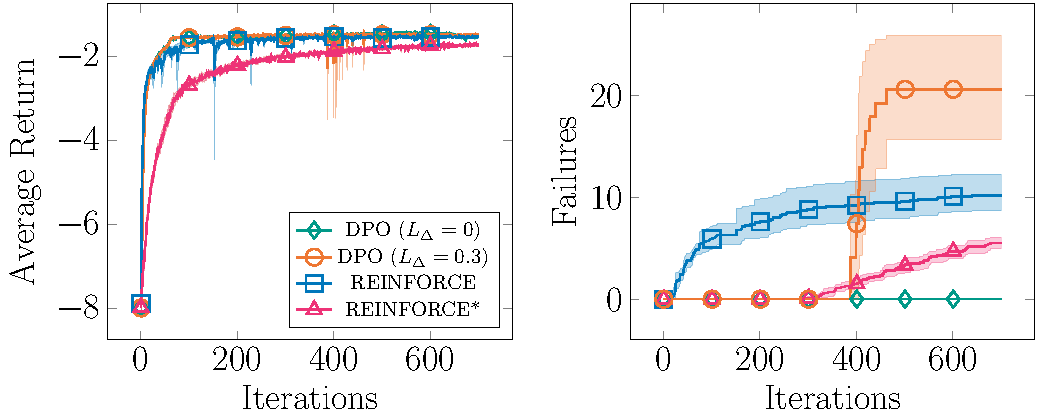
\includegraphics[width=\columnwidth]{plots/minigolf.pdf}
	\caption{Minigolf results, averaged over $10$ random seeds with $95\%$ bootstrapped confidence intervals. On the left: average return ($\gamma=0.99$) per iteration. On the right: number of failing episodes in a batch of $500$ (the same legend applies).}
	\label{fig:minigolf}
\end{figure}
%
%\subsection{Mobile Robot}
\paragraph{Robot Adaptation:}
Finally, we consider a more realistic scenario. A mobile robot on a flat surface has to reach goal areas specified by the user. 
The task is adapted from Safety Gym~\citep{ray2019benchmarking} and based on MuJoCo~\citep{todorov2012mujoco}. The robot has a speed-based actuator for turning and a force-based one for going forward and backward, resulting in a two-dimensional action. Its state is composed of typical sensor observations (accelerometer, velocimeter, gyroscope, magnetometer) and a compass pointing to the current goal, for a total of $9$ state variables. The goal is a randomly placed circular area, and the robot is rewarded for approaching it through a dense reward signal. Whenever reached, the goal is placed at a new random position. We initialize the robot with a good deterministic linear policy, learned with PGPE, whose performance (averaged over $1000$ test episodes) is reported as a black dashed line in Figure~\ref{fig:recover}. Imagine this policy has been learned in a controlled environment, then the robot has been deployed in a facility where random actions are not permitted. Then, a fault occurs, in the form of a fixed offset ($20\degree$) on the angle measured by the goal compass. The lower performance of the original policy after the fault is reported as a red dotted line. A corresponding difference in the agent's behavior can be appreciated from the attached videos (see Appendix~\ref{sec:app5}). Using DPO, the agent can adapt the policy parameters to the environmental change, as shown in Figure~\ref{fig:recover}. The environment is deterministic. We also make the simplifying assumption $L_{\Delta}=0$ and show the results for a hand-tuned regularization parameter $\lambda$. For each policy update, a batch of $10$ episodes of $200$ steps each is collected, and we show the average return over each batch. The performance of PGPE is also reported as a reference. Both algorithms are able to fine-tune the policy back to its original performance. However, DPO does that without action randomization.

\begin{figure}[t]
	\begin{minipage}[t]{.48\columnwidth}
		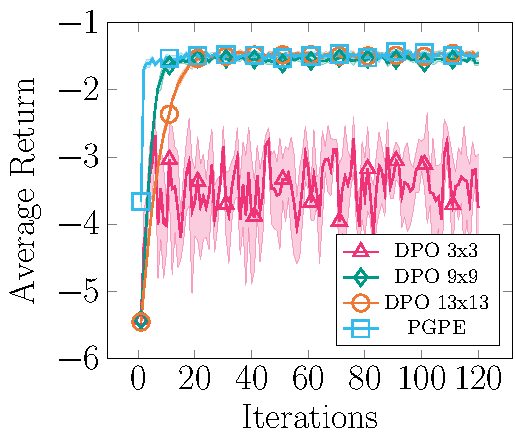
\includegraphics[width=\textwidth]{plots/mass.pdf}
		\caption{Double Integrator: average return ($\gamma=0.95$) per iteration, averaged over $5$ random seeds with $95\%$ bootstrapped confidence intervals.}
		\label{fig:mass}
	\end{minipage}%
	\hfill
	\begin{minipage}[t]{.48\columnwidth}
		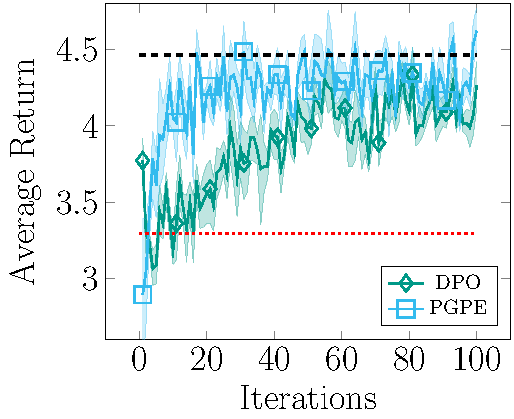
\includegraphics[width=\textwidth]{plots/recover.pdf}
		\caption{Robot Adaptation: average return (undiscounted) per iteration, averaged over $10$ random seeds with $95\%$ bootstrapped confidence intervals.}
		\label{fig:recover}
	\end{minipage}
\end{figure}

\section{Task Specifications}\label{sec:app3}
In this section, we provide further details on the environment simulators and the policies used to perform the experiments.

\subsection{Minigolf}
The state space is one-dimensional and represented by the interval $(0,20]$. States whose value is greater than 20 are set to 20, states whose value is lower or equal to 0 cause the end of the episode. The action space is one-dimensional and represented by the interval $[10^{-5}, 5]$. Actions whose value is outside from the interval are clipped. The environment is deterministic, with a function $f(s,a)$ that exactly computes the arriving state $s'$ from every pair $(s,a)$:
\[
s'=f(s,a) = s - at + 0.5 \times dt^2,
\]
where $t=\frac{a}{d}$ and $d = \frac{5}{7} \times friction(s) \times 9.81$.
Friction is computed as:
\[
friction(s) = friction\_low + \frac{friction\_high - friction\_low}{s_{max} - s_{min}} \times s
\]
where $friction\_low=0.131$, $friction\_high=0.19$, $s_{max}=20$ and $s_{min}=0$. The Lipschitz constant $L_{\Delta}$ of the environment is computed as follows:\\
\begin{align}
\Delta(s,a) = -0.5 \times \frac{a^2}{d(s)}; &\quad friction(s) = 0.131 + 2.95 \times 10^{-3} \times s, \nonumber\\
\norm{\Delta(s,a) - \Delta(\wt{s},a)} &= \norm{ -0.5 \times a^2 \Big(\frac{1}{7 \times friction(s)} - \frac{1}{7 \times friction(\wt{s})} \Big)} \nonumber\\
&= \norm{-0.0714 \times a^2}\norm{\frac {2.95 \times 10^{-3} \times (\wt{s} -s)} {friction(s) \times friction(\wt{s})}}\label{p:31}\\
&= L_{\Delta} \norm{s - \wt{s}} \quad \text{ with }L_{\Delta}=0.3, \label{p:32}
\end{align}
where~\eqref{p:32} is obtained from~\eqref{p:31} considering the maximum possible value for actions and the minimum possible value for states, so as to maximize $L_{\Delta}$.
At any time step, the reward function depends only on the current state: the effect of every action performed is observable in the reward of the next step of the episode: 
\begin{align}
R(s) = 
\begin{cases}
0 & \text{if } s \in [-4,0],\\
-100 & \text{if } s < -4,\\
-1 & \text{otherwise}.
\end{cases} \nonumber
\end{align}

The policy used for this task is a radial-basis network composed of four Gaussian functions $\phi_i$, with constant hyper-parameters $\mu_i$ and $\sigma_i$. The action prescribed by the policy is computed as $a = \vphi(s)^T\vtheta$, where $\vtheta\in\Reals^4$, the learned parameters, are the weights given to each Gaussian function. The initial values for $\vtheta$ are $[1, 1, 1, 1]$. The RBF hyperparameters are as follows: 
\begin{align}
\phi_i(s; \mu_i, \sigma_i) &= \exp\left\{-{(s -\mu_i)^2}\big/{(2\sigma_i^2)}\right\}, \nonumber \\
\mu_i &\in (4, 8, 12, 16), \nonumber \\
\sigma_i &\in(4, 4, 4, 4). \nonumber
\end{align}
In the case of REINFORCE, a Gaussian noise $\eta\sim\Gauss(0,\sigma^2)$ is added to the action, where $\sigma=e^{\omega}$ and $\omega\in\Reals$ is an additional learned parameter. The initial value for $\sigma$ is selected as a hyper-parameter.

We set a discount factor of $\gamma=0.99$ and a maximum task horizon of $20$ time steps.

\subsection{Double Integrator}\label{sec:di}
The environment has a two-dimensional state and a scalar action. 
Both the state dimensions and the actions are represented with real values in the interval $[-1, 1]$. The arriving state $s'$ is computed with the following equation:
\begin{align}
s' &= As + Ba + \epsilon, \qquad \epsilon\sim\Gauss(0,\nu^2),\nonumber
\end{align}
where:
\begin{align}
&\quad A =
\begin{bmatrix}
1 & \tau \\
0 & 1 
\end{bmatrix}, &\quad 
B =
\begin{bmatrix}
0 \\
\frac{\tau}{mass} 
\end{bmatrix},\nonumber
\end{align}
$\nu=0.1$, $mass=1$ and $\tau = 1$.
Since the term $\epsilon$ is a Gaussian noise, $P(s'|s,a)$ will be a Gaussian distribution.
The reward function is:
\begin{align}
R(s) &= - (s^TQs + ara),\nonumber\\
\end{align}
where:
\begin{align}
Q =
\begin{bmatrix}
1 & 0 \\
0 & 0
\end{bmatrix},
\end{align}
and $r = 0.1 $.
The policy used for this task is linear in the state, with initial parameters = $[-0.3, -0.3]$. For PGPE, a factored Gaussian hyper-policy $\Gauss(\boldsymbol{\rho},\mathop{diag}(\boldsymbol{\sigma}^2)$ is defined over the two-dimensional parameter space, where $\boldsymbol{\sigma}=e^{\boldsymbol{\omega}}$, $\boldsymbol{\rho},\boldsymbol{\omega}\in\Reals^2$ are learned parameters, and $\boldsymbol{\rho}$ is always initialized to $[-0.3,-0.3]$. Both the components of $\boldsymbol{\sigma}$ are initialized to the same scalar $\sigma$, selected as a hyper-parameter. 

We set a discount factor of $\gamma=0.95$ and a maximum task horizon of $20$ time steps.

\subsection{Robot Adaptation}\label{sec:robot}
This is a custom environment built using the Safety Gym library~\citep{ray2019benchmarking}, which relies on the MuJoCo simulator~\citep{todorov2012mujoco}. The task is composed by a mobile robot that moves on a flat surface with the aim of reaching a randomly placed goal area. The state space considered in the task is composed by $9$ variables that represent the measurements of some sensors mounted on the robot. The robot is equipped with four standard sensors (accelerometer, velocimeter, gyroscope, magnetometer) and a compass that detects the orientation of the robot with regard to the goal area. Since the environment is flat, some of the data coming from the sensor (\eg vertical acceleration) are unnecessary and are simply discarded in order to reduce the dimensionality of the state space. 
The reduced state is composed by the following variables, reported here in the order in which they are considered in the implementation. All measurements are in the robot's frame of reference:
\begin{itemize}
	\item Linear acceleration in the plane (coordinates of a $2$D vector).
	\item Cosine and sine of the angle observed by the compass, which indicates the direction of the goal.
	\item Angular velocity of the robot (\wrt yaw);
	\item Magnetic flux observed by the magnetometer (coordinates of a $2$D vector).
	\item Linear velocity in the plane (coordinates of a $2$D vector).
\end{itemize}
Note that the robot has no information regarding its position in the world's frame of reference, which is not necessary for this task.
The reward function is defined as:
\[ 
R(s_t, a_t) = r \times \Delta distance\_from\_goal(t),
\]
where $r=1$, $\Delta distance\_from\_goal = distance(t) - distance(t-1)$ and $distance(t)$ measures the distance of the robot from the goal at time step $t$.
To compute $\Delta distance\_from\_goal$, the environment keeps a memory of previous distances. This, together with the fact that $distance(t)$ cannot be computed from the available observations, prevents us to compute $R(s,a)$ for all states and actions, as assumed in the paper. However, since $R(s_t,a_t)$ is independent from $a_t$, we can estimate $R(X,a)$ for any abstract state $X$ and action $a$ simply by averaging the rewards obtained in the states of $X$, regardless of the performed action. The delayed effect of actions on rewards is captured by also estimating the abstract transition function anyway.

For this task, we use a linear policy. The initial parameters, learned with PGPE and representing an almost optimal policy before the compass fault, are reported here:
\[
\vtheta_{0} = 
\begin{bmatrix}
0.108& 0.022& 4.301& 0.108& 0.017& 0.112& 0.019& -0.179& -0.038\\
-0.004& 0.486& 0.105& -12.069& 1.070& -0.047& -0.222& 0.036& -0.398\\
\end{bmatrix}.
\]
For PGPE, a factored Gaussian hyper-policy $\Gauss(\boldsymbol{\rho},\mathop{diag}(\boldsymbol{\sigma}^2))$ is defined over the $18$-dimensional parameter space, where $\boldsymbol{\sigma}=e^{\boldsymbol{\omega}}$, $\boldsymbol{\rho},\boldsymbol{\omega}\in\Reals^{18}$ are learned parameters, and $\boldsymbol{\rho}$ is initialized as $\vtheta_{0}$. All the components of $\boldsymbol{\sigma}$ are initialized to the same scalar $\sigma$, selected as a hyper-parameter.

We set a discount factor of $1$ and a maximum task horizon of $200$ ($2000$ in some experiments) time steps.


\section{Experimental Details}\label{sec:app4}

In this section we provide further details on how the experiments presented in the paper were conducted. 

\subsection{Hyper-parameter tuning}
For each task, we have to tune some hyper-parameters before applying the different algorithms. We do so via \emph{grid search}. We define a set of reasonable values for these parameters and we fix a criterion for choosing the best parameters to be used in the algorithm. We compute the sum over $n$ iterations of the performance measure (estimated from the collected samples at each iteration of the algorithm) and average it over $m$ independent runs, performed with different random seeds. 
The values of $n$ and $m$ for the different experiments, together with other details, are reported in Table~\ref{tab:recap1}.
The results of the grid search are reported in Tables~\ref{tab:t1}-\ref{tab:t5}.
The bold values in the tables represent the combination of parameters used to perform the final experiments. For REINFORCE~\citep{williams1992simple}, the selected hyper-parameters are the step size $\alpha$ and the policy initial standard deviation $\sigma$. For DPO, the learning rate $\alpha$ of the projection phase and the regularization coefficient $\lambda$ (see Section~\ref{sec:detail}). For PGPE~\citep{sehnke2008policy}, the step size $\alpha$ and the hyper-policy initial standard deviation $\sigma$.

\begin{table}
	\centering
	\begin{tabular}{ll|cccccc}
		\toprule
		\textbf{Task} & \textbf{Algorithm} & $n$ & $m$ & $N$ & $H$ & $\gamma$ & $|\Xspace|$\\
		\midrule
		Minigolf & DPO & $300$ & $5$ & $500$ & 20 & $0.99$ & $12$ \\
		& REINFORCE & $300$ & $5$ & $500$ & 20 & $0.99$ & -- \\
		Double Integrator & DPO & $60$ & $3$ & $500$ & $20$ & $0.95$ & $9^{2}$ \\
		& PGPE & $100$ & $5$ & $500$ & $20$ & $0.95$ & -- \\
		Robot Adaptation & DPO & $500$ & $5$ & $1$ & $2000$ & $1$ & $5^{9}$ \\
		& PGPE & $100$ & $5$ & $10$ & $200$ & $1$ & --\\
		\midrule
	\end{tabular}
	\caption{\label{tab:recap1}Configurations used for hyper-parameter tuning. We denote with $n$ the number of iterations (policy updates), with $m$ the number of independent runs, with $N$ the batch size, with $H$ the task horizon, with $\gamma$ the discount factor and with $|\Xspace|$ the number of abstract states.}
\end{table}

\subsection*{Minigolf}
For REINFORCE (Table~\ref{tab:t2}) we performed the final experiment with two different combinations of parameters: $(\alpha=0.05, \log\sigma=-2)$ selected according to the criterion used in the tuning phase and $(\alpha=0.005, \log\sigma=-3)$, that provided the lowest number of \emph{failures} in the tuning phase.
\begin{table}[H]
	\parbox{.45\linewidth}{
		\centering
		\begin{tabular}{l|*{3}{c}}
			\toprule
			\backslashbox{$\alpha$}{$\lambda$}
			&0.0005&0.001&0.005\\
			\midrule
			0.001 & \textbf{-524.69} & -526.51 & -538.16 \\
			0.005 & -529.29 & -530.28 & -533.53 \\
			0.01 & -572.35 & -573.54 & -566.87 \\
			\bottomrule
		\end{tabular} \caption{\label{tab:t1} Grid search for DPO on Minigolf.}
	}
	\hfill
	\parbox{.45\linewidth}{
		\centering
		\begin{tabular}{l|*{3}{c}}
			\toprule
			\backslashbox{$\alpha$}{$\log\sigma$}
			&-4&-3&-2\\
			\midrule
			0.005 & -897.95 & \textbf{-883.72} & -876.55 \\
			0.01 & -1011.65 & -744.81 & -734.89 \\
			0.05 & -4971.86 & -2965.25 & \textbf{-551.86} \\
			\bottomrule
		\end{tabular} \caption{\label{tab:t2}Grid search for REINFORCE on Minigolf.}
	}
\end{table}

\subsection*{Double Integrator} 
Hyper-parameter selection was performed for the $9\times 9$ discretization, and kept fixed in the final experiments for other discretizations. We used a fixed $\alpha$ (also for the next task) since its effects on performance are negligible. 
\begin{table}[H]
	\parbox{.45\linewidth}{
		\centering
		\begin{tabular}{l|*{3}{c}}
			\toprule
			\backslashbox{$\alpha$}{$\lambda$}
			&0.0001&0.0005&0.001\\
			\midrule
			0.025 & \textbf{-94.76} & -95.91 & -97.80 \\
			\bottomrule
		\end{tabular} \caption{\label{tab:t3}Grid search for DPO on Double Integrator.}
	}
	\hfill
	\parbox{.45\linewidth}{
		\centering
		\begin{tabular}{l|*{3}{c}}
			\toprule
			\backslashbox{$\alpha$}{$\sigma$}
			&0.1&0.5&1\\
			\midrule
			0.1 & -187.86 & -184.57 & -190.18 \\
			0.5 & -174.69 & -158.39 & -161.64 \\
			1 & -169.29 & \textbf{-153.93}	 & -159.28 \\
			\bottomrule
		\end{tabular} \caption{\label{tab:t6}Grid search for PGPE on Double Integrator.}
	}
\end{table}

\subsection*{Robot Adaptation}
To verify the convergence of DPO, we run it on a longer number of iterations than PGPE. We also used a single, longer episode per iteration, which is more realistic. However, these settings were aligned for the final experiments, to make the comparison fair.
\begin{table}[H]
	\parbox{.45\linewidth}{
		\centering
		\begin{tabular}{l|*{3}{c}}
			\toprule
			\backslashbox{$\alpha$}{$\lambda$}
			&0.001&0.01&0.05\\
			\midrule
			0.005 & 20658.70 & 23163.38 & \textbf{23553.37} \\
			\bottomrule
		\end{tabular} \caption{\label{tab:t4}Grid search for DPO on Robot Adaptation.}
	}
	\hfill
	\parbox{.45\linewidth}{
		\centering
		\begin{tabular}{l|*{3}{c}}
			\toprule
			\backslashbox{$\alpha$}{$\sigma$}
			&0.1&0.5&1\\
			\midrule
			0.1 & 337.33 & 378.27 & 358.08 \\
			0.5 & 372.23 & 413.78 & 402.46 \\
			1 & 395.88 & \textbf{419.37}	 & 405.55 \\
			\bottomrule
		\end{tabular} \caption{\label{tab:t5}Grid search for PGPE on Robot Adaptation.}
	}
\end{table}

\subsection{Final Experiments}
The results of the final experiments (averaged over multiple runs performed with separate random seeds) are reported in Section~\ref{sec:exp}. 
%Any differences among the algorithms on the same task (except from the selected hyper-parameters) that existed in the tuning phase were removed in the final experiments for fair comparison. 
We recap the final configurations in Table~\ref{tab:recap2} for the sake of reproducibility.

\begin{table}[h!]
	\centering
	\begin{tabular}{ll|ccccccccc}
		\toprule
		\textbf{Task} & \textbf{Algorithm} & $\alpha$ & $\lambda$ & $\sigma$ & $n$ & $m$ & $N$ & $H$ & \textbf{$\gamma$} & $|\Xspace|$\\
		\midrule
		Minigolf & DPO & $0.001$ & $0.0005$ & -- & $700$ & $10$ & $500$ & 20 & $0.99$ & $12$ \\
		& REINFORCE & $0.05$ & -- & $e^{-2}$ & $700$ & $10$ & $500$ & 20 & $0.99$ & -- \\
		& REINFORCE* & $0.005$ & -- & $e^{-3}$ & $700$ & $10$ & $500$ & 20 & $0.99$ & -- \\
		\midrule
		Double Integrator & DPO & $0.025$ & $0.0001$ & -- & $120$ & $5$ & $500$ & $20$ & $0.95$ & $\{3^{2},9^{2},13^{2}\}$ \\
		& PGPE & $1$ & -- & $0.5$ & $120$ & $5$ & $500$ & $20$ & $0.95$ & -- \\
		\midrule
		Robot Adaptation & DPO & $0.005$ & $0.05$ & -- & $100$ & $10$ & $10$ & $200$ & $1$ & $5^{9}$ \\
		& PGPE & $1$ & -- & $0.5$ & $100$ & $10$ & $10$ & $200$ & $1$ & --\\
		\midrule
	\end{tabular}
	\caption{\label{tab:recap2}Configurations used for hyper-parameter tuning, including hyper-parameters $\alpha$, $\lambda$ and $\sigma$. We denote with $n$ the number of iterations (policy updates), with $m$ the number of independent runs, with $N$ the batch size, with $H$ the task horizon, with $\gamma$ the discount factor and with $|\Xspace|$ the number of abstract states.}
\end{table}


\section{Additional Results}\label{sec:app5}
In this section, we provide additional results on DPO, with the purpose of better understanding its workings in practice. 

\subsection{Abstract state-space visualization in Robot Adaptation}
The Robot Adaptation task has a $9$-dimensional state space, discretized into a Cartesian grid of $5$ buckets per dimension. The total number of abstract states is very large ($\sim 10^{6}$) and could cause computational issues. However, as mentioned, only a subset of the abstract state space is actually visited by the agent and needs to be considered in the computations of DPO. The colormaps of Figures~\ref{fig:cm0}-\ref{fig:cm99} show the visitation frequencies, for different iterations of the algorithm, of the abstract states, projected onto two of the most relevant state variables (the goal compass measurements) for visualization purposes. Axes labels are the bucket indexes, and the values are the ratios of total visits over $2000$ time steps, averaged over $10$ episodes. We can see that some abstract states are not visited at all. These are ignored in the estimation of the abstract transition and reward functions, in the value iteration phase and in the projection phase. Note how the visits change across iterations, and some previously ignored abstract states must be added to the abstract MDP. The central states are never visited, as they correspond to unfeasible configurations (the two variables are the sine and cosine of an angle and their squares must always sum to one). We can also see an improvement in the agent's behavior: abstract state $(0,2)$ (the most visited one) corresponds to the agent facing the goal. After $99$ iterations, the visitation frequency of this state has significantly increased, meaning that the agent is able to point to the goal very quickly. This can also be seen from the videos of Section~\ref{sec:videos}.


\subsection{Abstract policy visualization in Minigolf}
In Figures~\ref{fig:mg0}-\ref{fig:mg499} we visualize the policies (abstract and concrete) learned by DPO, for different iterations of the Minigolf experiment. The plots have the original state space on the horizontal axis and the continuous action space on the vertical one (both are one-dimensional in this task). The red line represents the deterministic policy, which is linear in a vector of Gaussian radial-basis features (hence non-linear in the state). White boxes correspond to the $12$ abstract states and represent the restricted action space considered in the value iteration phase. Blue boxes represent the range of optimal actions obtained via value iteration. Note that, in this task, several optimal abstract policies exist. These are all considered as valid targets in the projection phase, in order to make the projection to the original policy space easier. The dotted line denotes the maximum action allowed by the environment (larger actions are clipped). When the box is placed above the dotted line, then, all the actions should be considered as optimal. This is not the case of the rightmost box in Figures~\ref{fig:mg399} and~\ref{fig:mg499}, where only a subset of the actions above the dotted line is considered as optimal. Indeed, by solving the task with $L_{\Delta}=0$, we assume that the friction has the same effect everywhere in the abstract state, which is not true in general. As a result, actions sampled where the friction is lower are evaluated better than they are.


\begin{figure}[h!]
	\centering
	\begin{minipage}[t]{.45\columnwidth}
		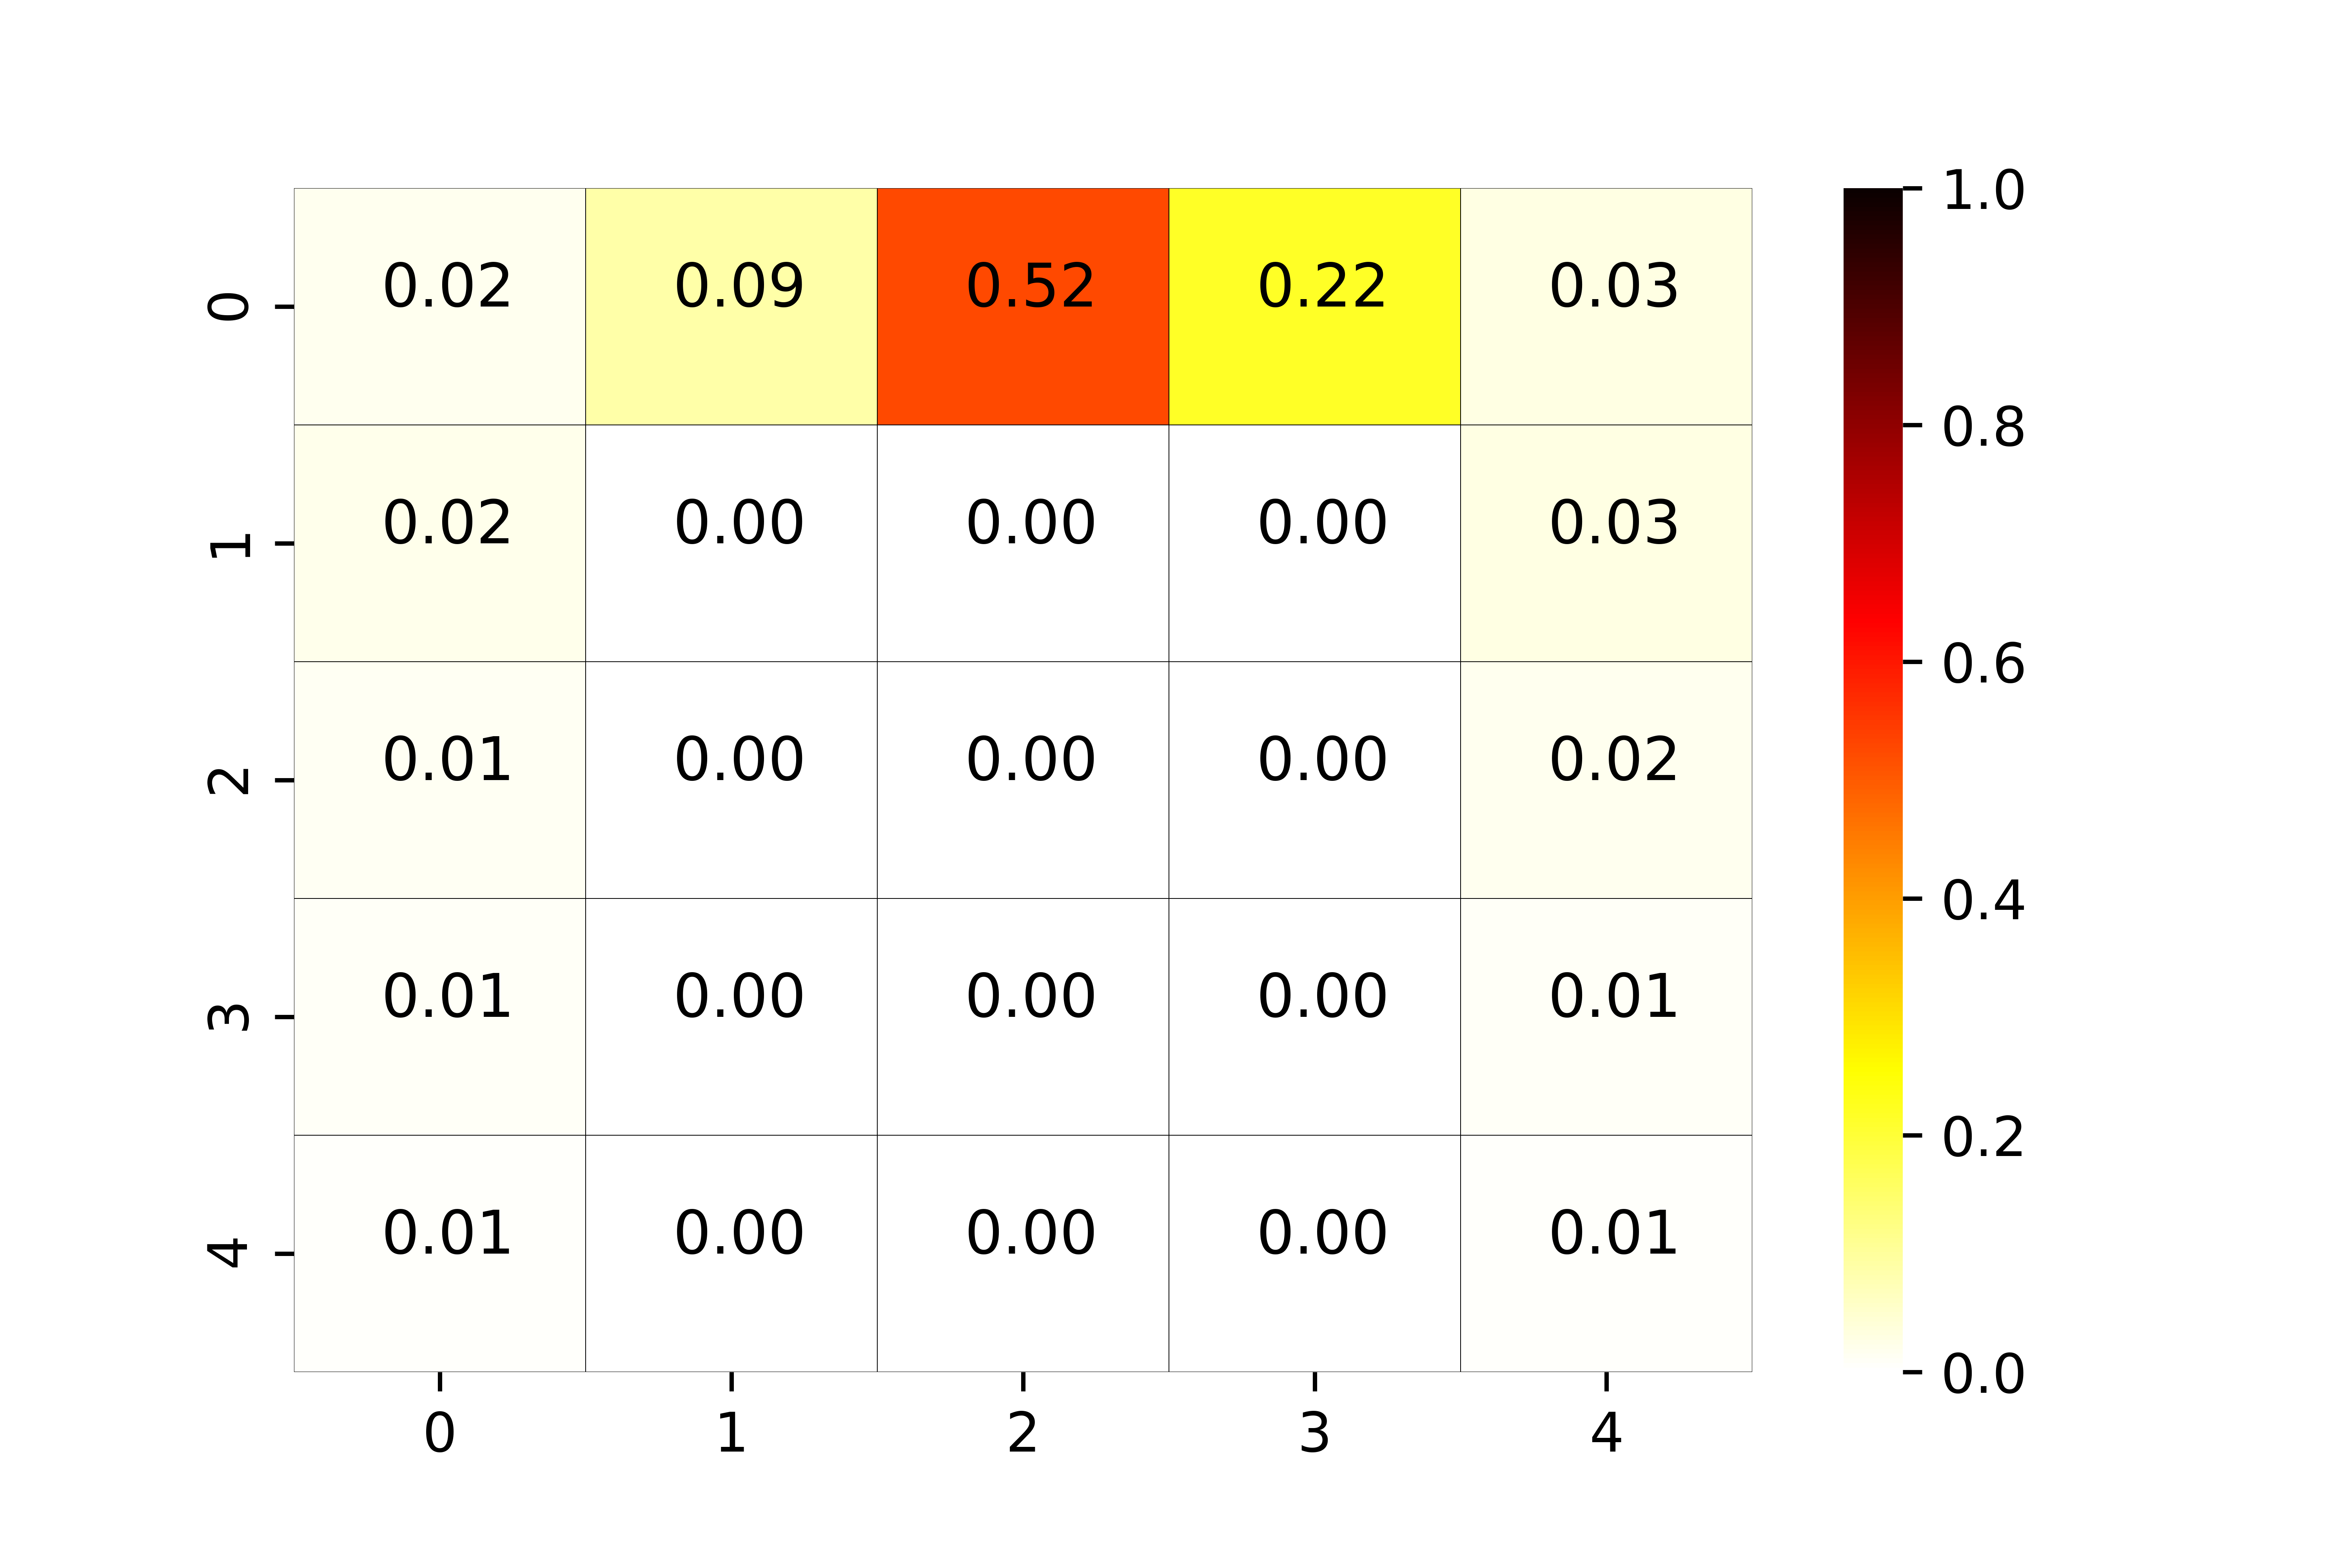
\includegraphics[width=\textwidth]{plots/colormap0.png}
		\caption{Robot Adaptation: abstract state visitation frequencies at the initial iteration of DPO.}
		\label{fig:cm0}
	\end{minipage}%
	\hfill
	\begin{minipage}[t]{.45\columnwidth}
		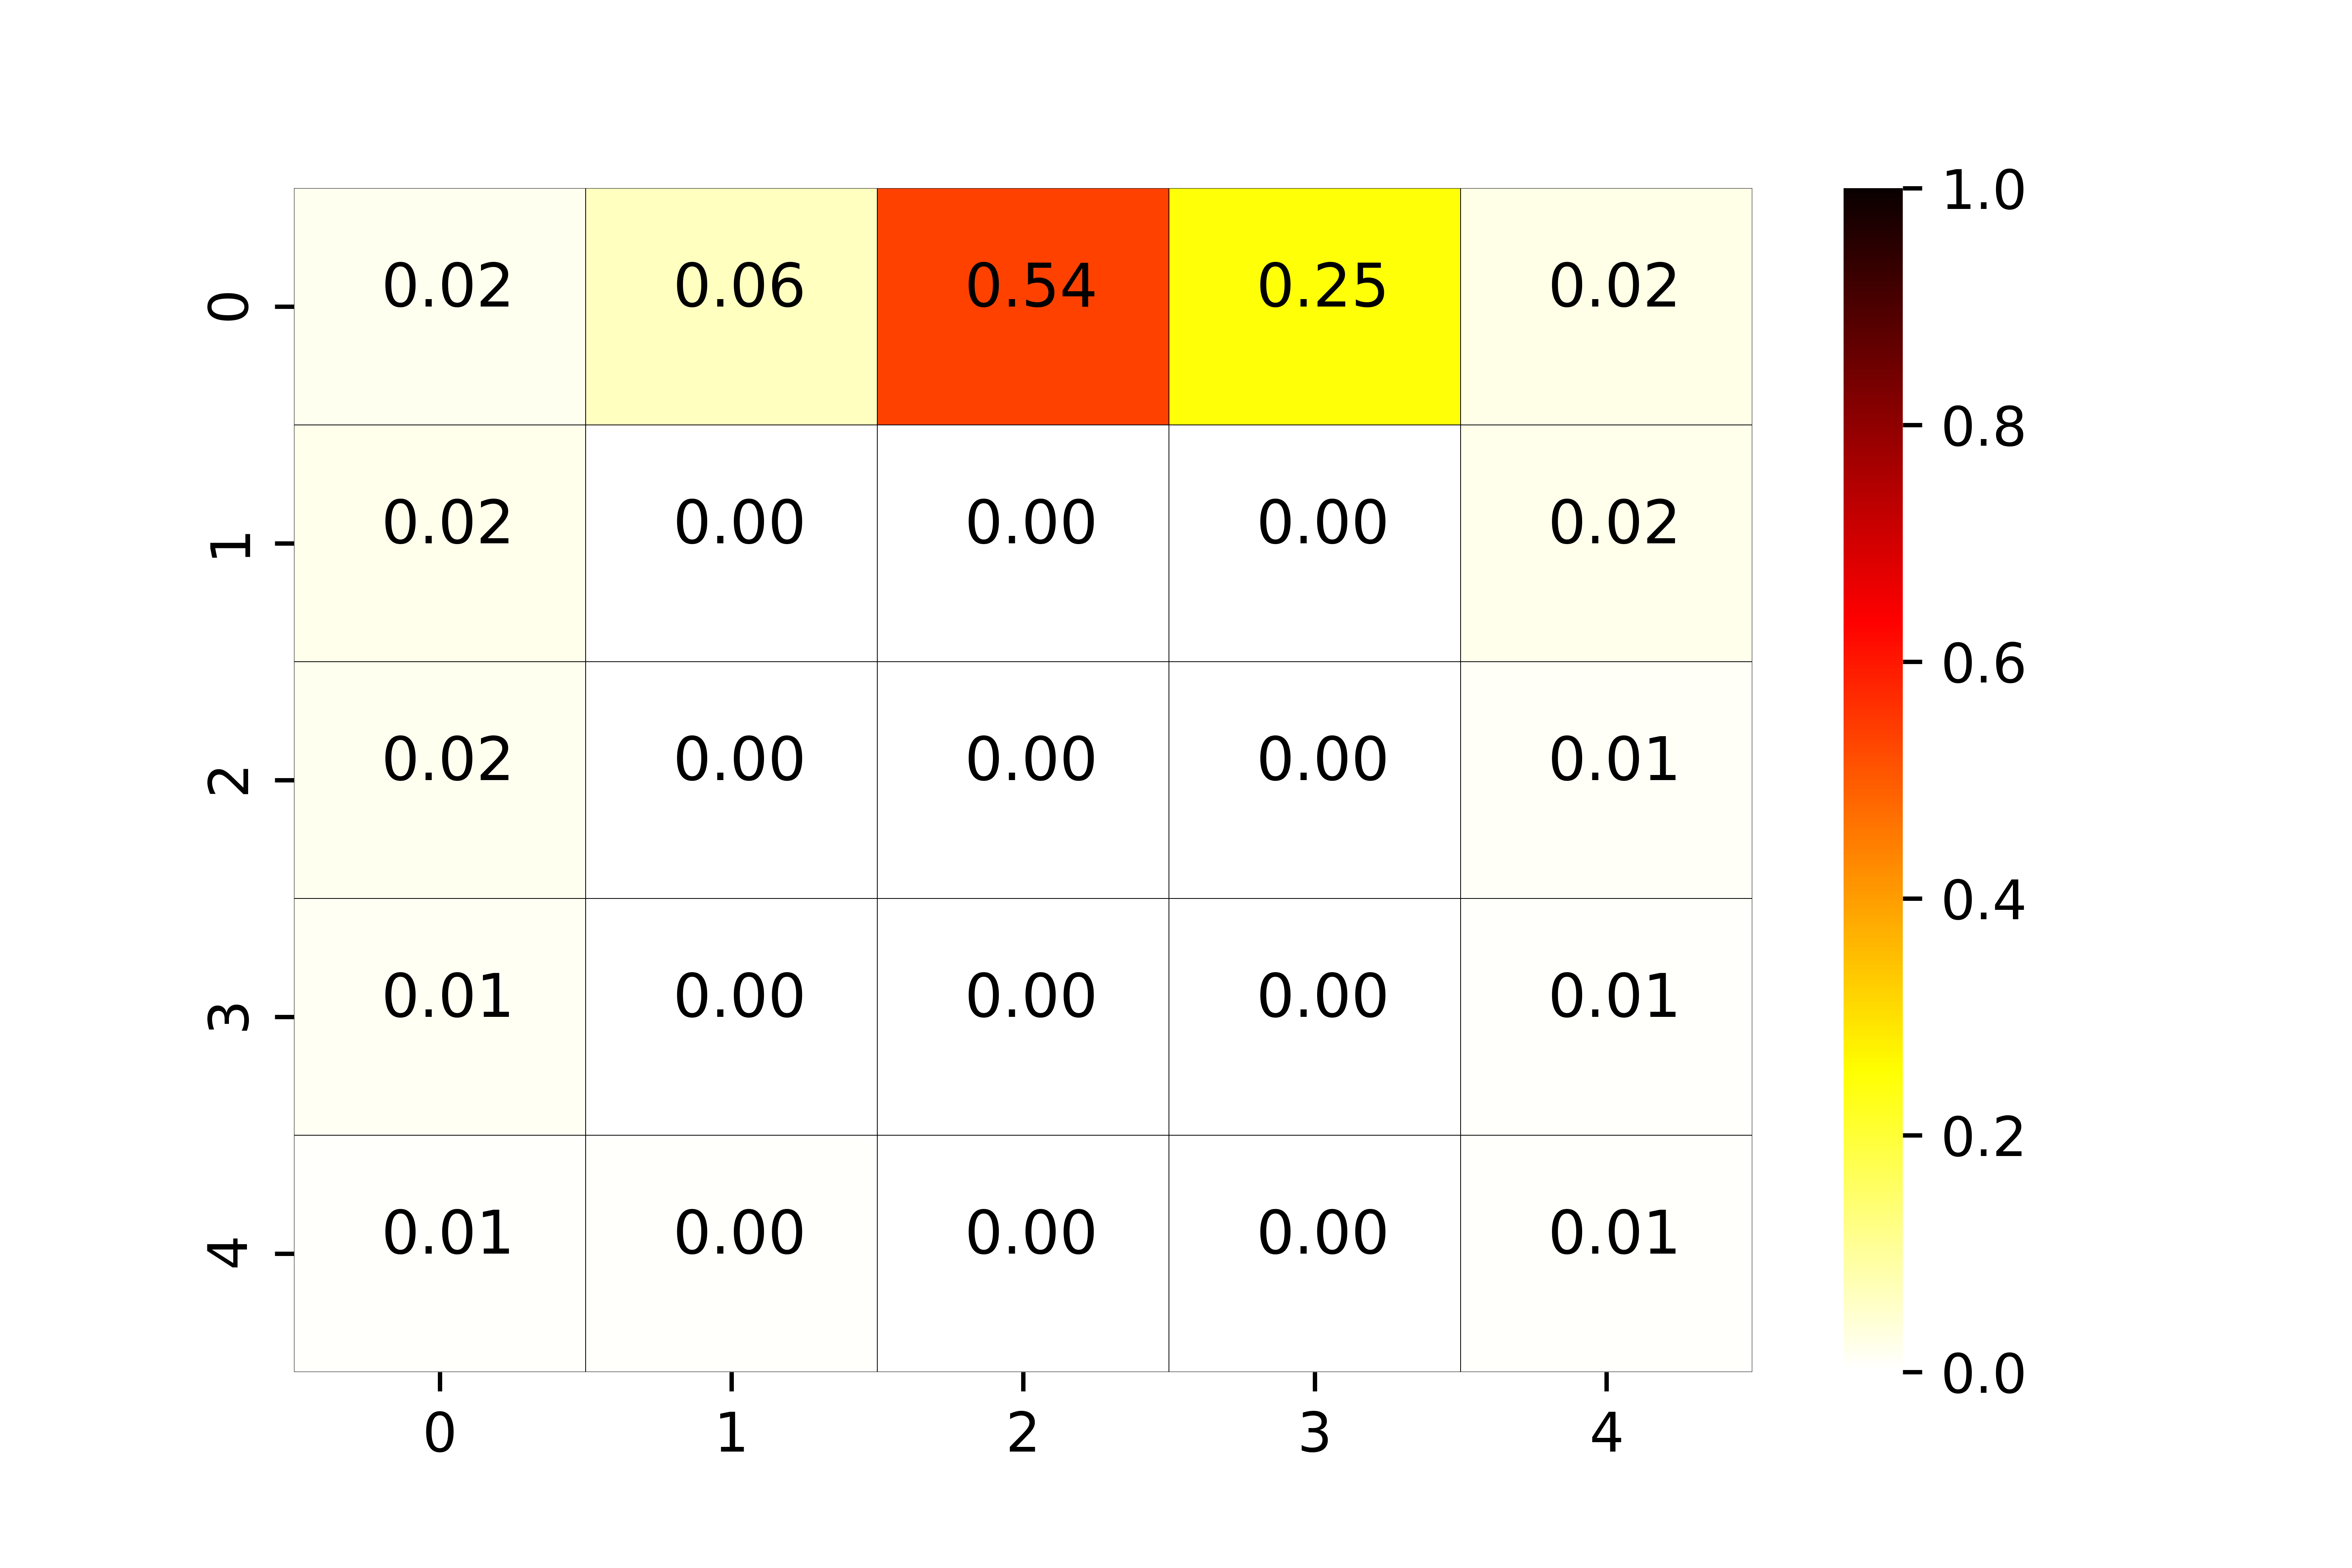
\includegraphics[width=\textwidth]{plots/colormap5.png}
		\caption{Robot Adaptation: abstract state visitation frequencies at the fifth iteration of DPO.}
		\label{fig:cm5}
	\end{minipage}
\end{figure}
\begin{figure}[h!]
	\centering
	\begin{minipage}[t]{.45\columnwidth}
		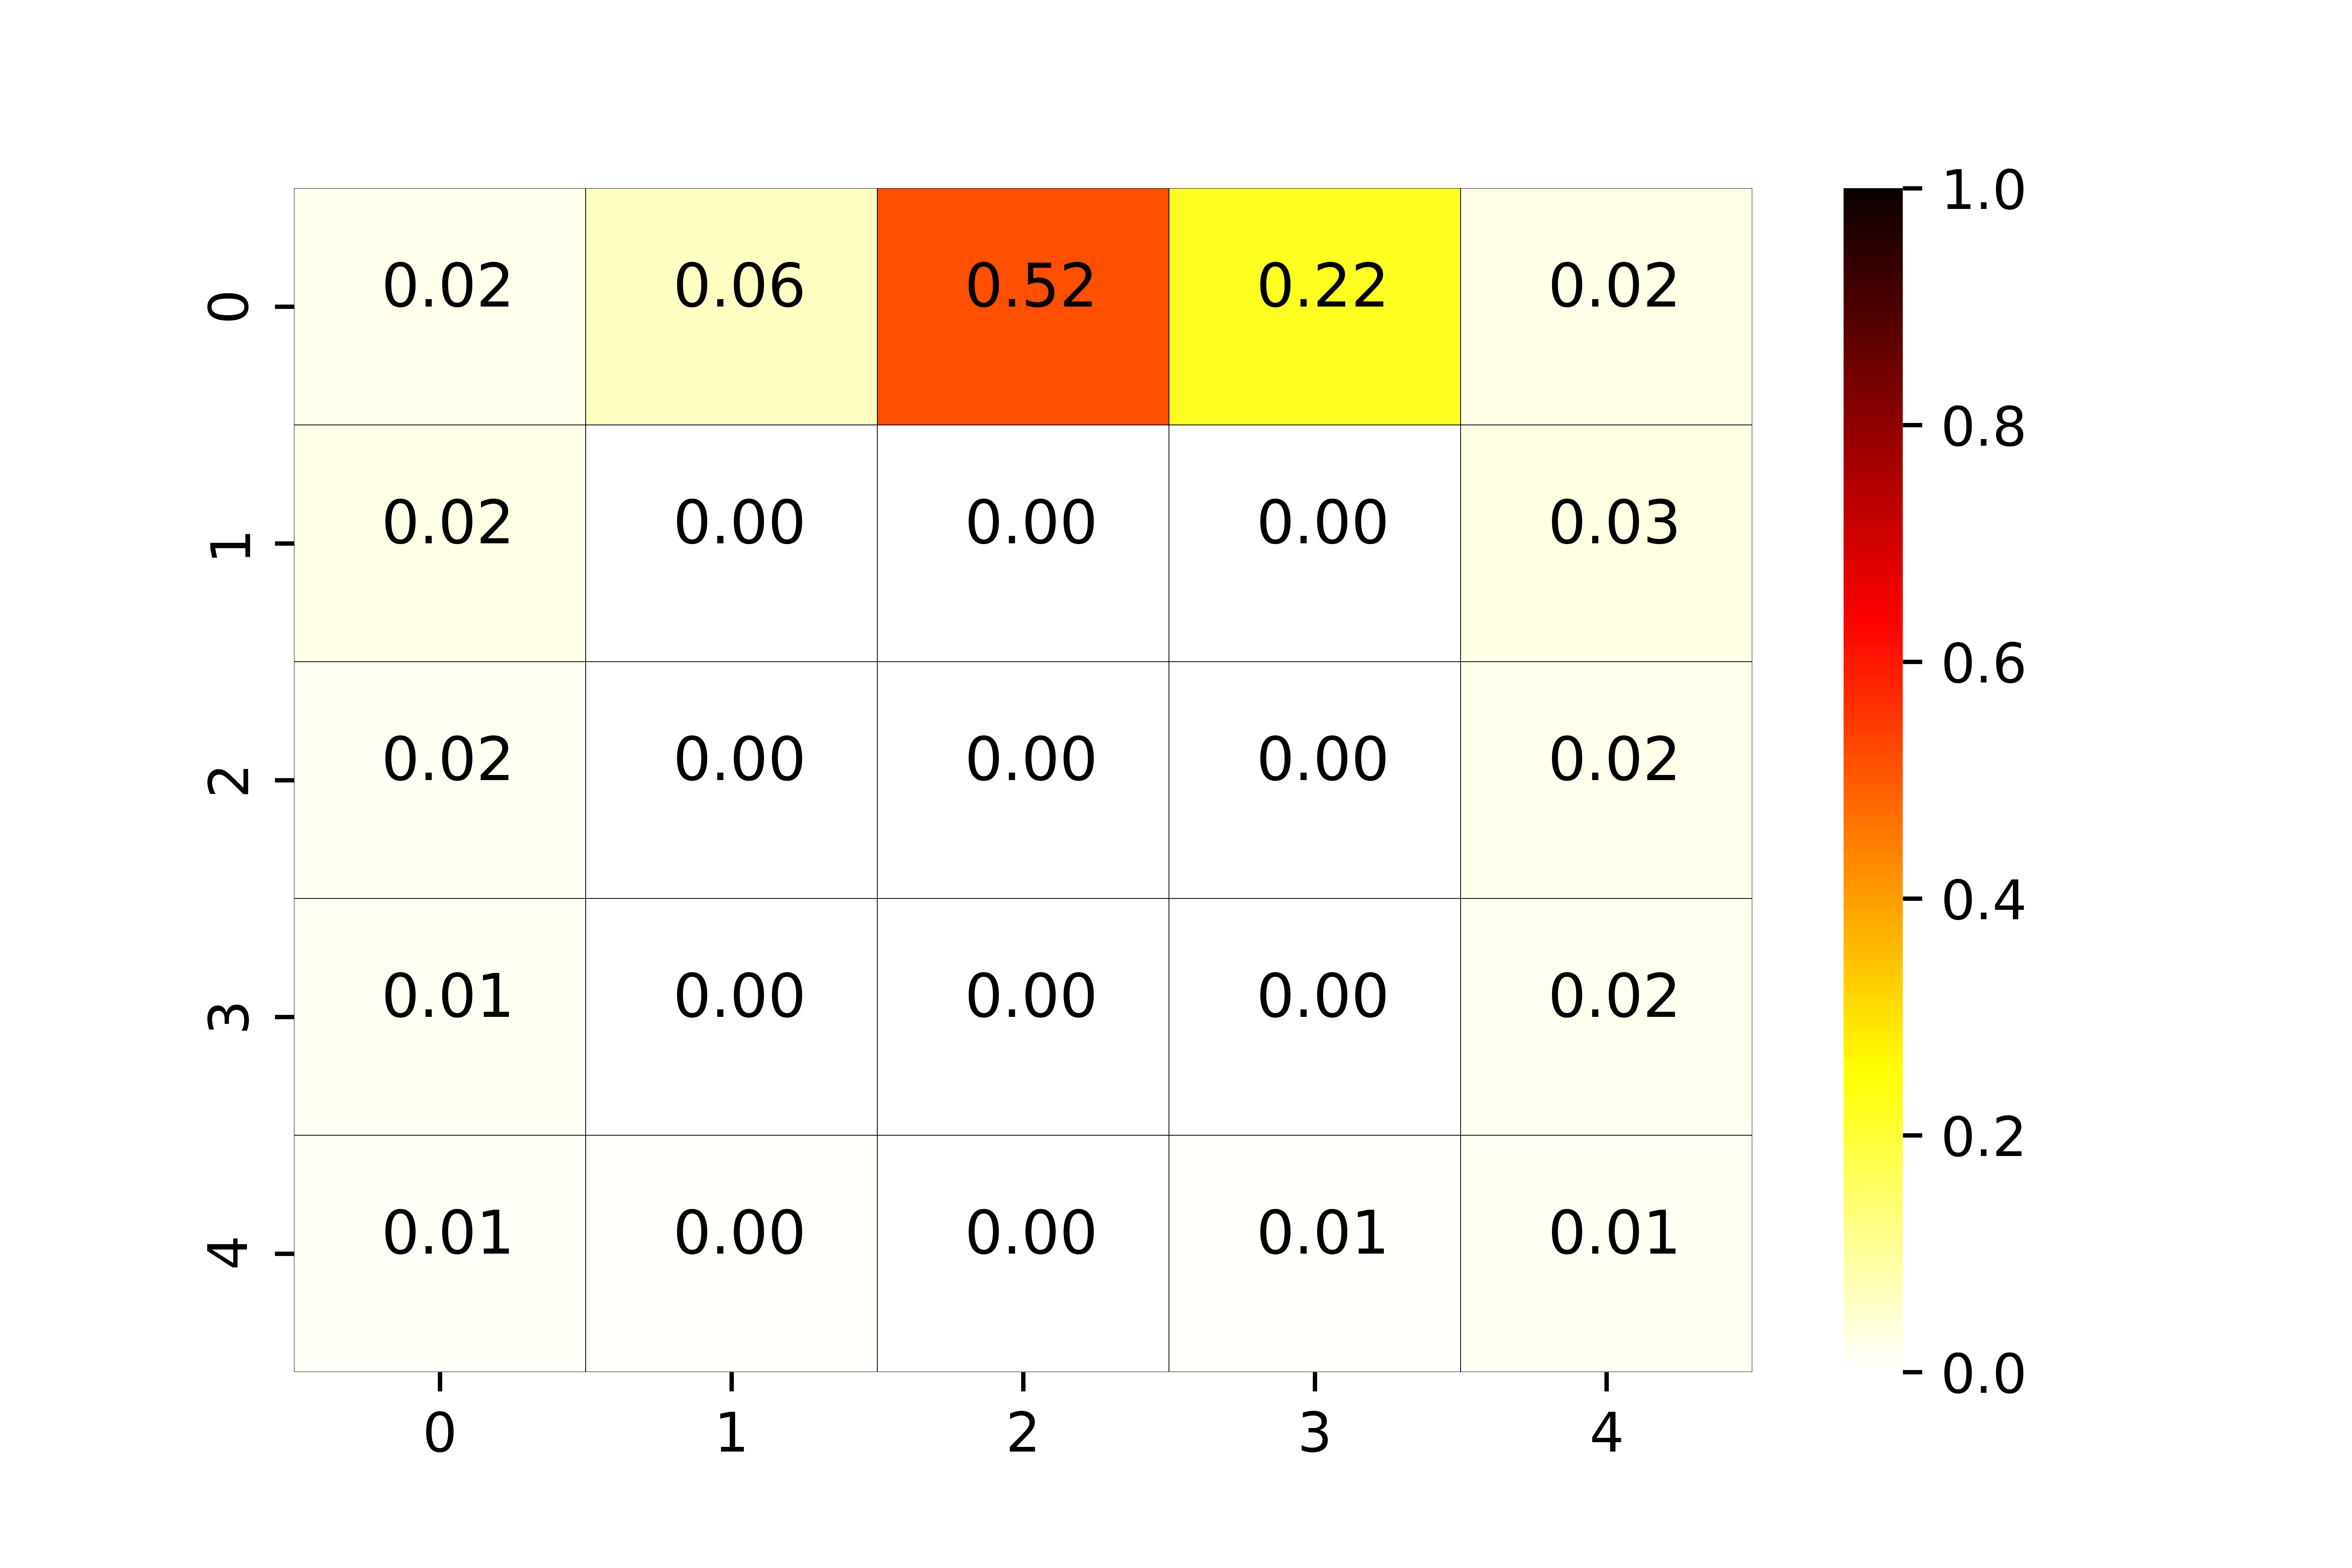
\includegraphics[width=\textwidth]{plots/colormap8.png}
		\caption{Robot Adaptation: abstract state visitation frequencies at the eighth iteration of DPO.}
		\label{fig:cm8}
	\end{minipage}%
	\hfill
	\begin{minipage}[t]{.45\columnwidth}
		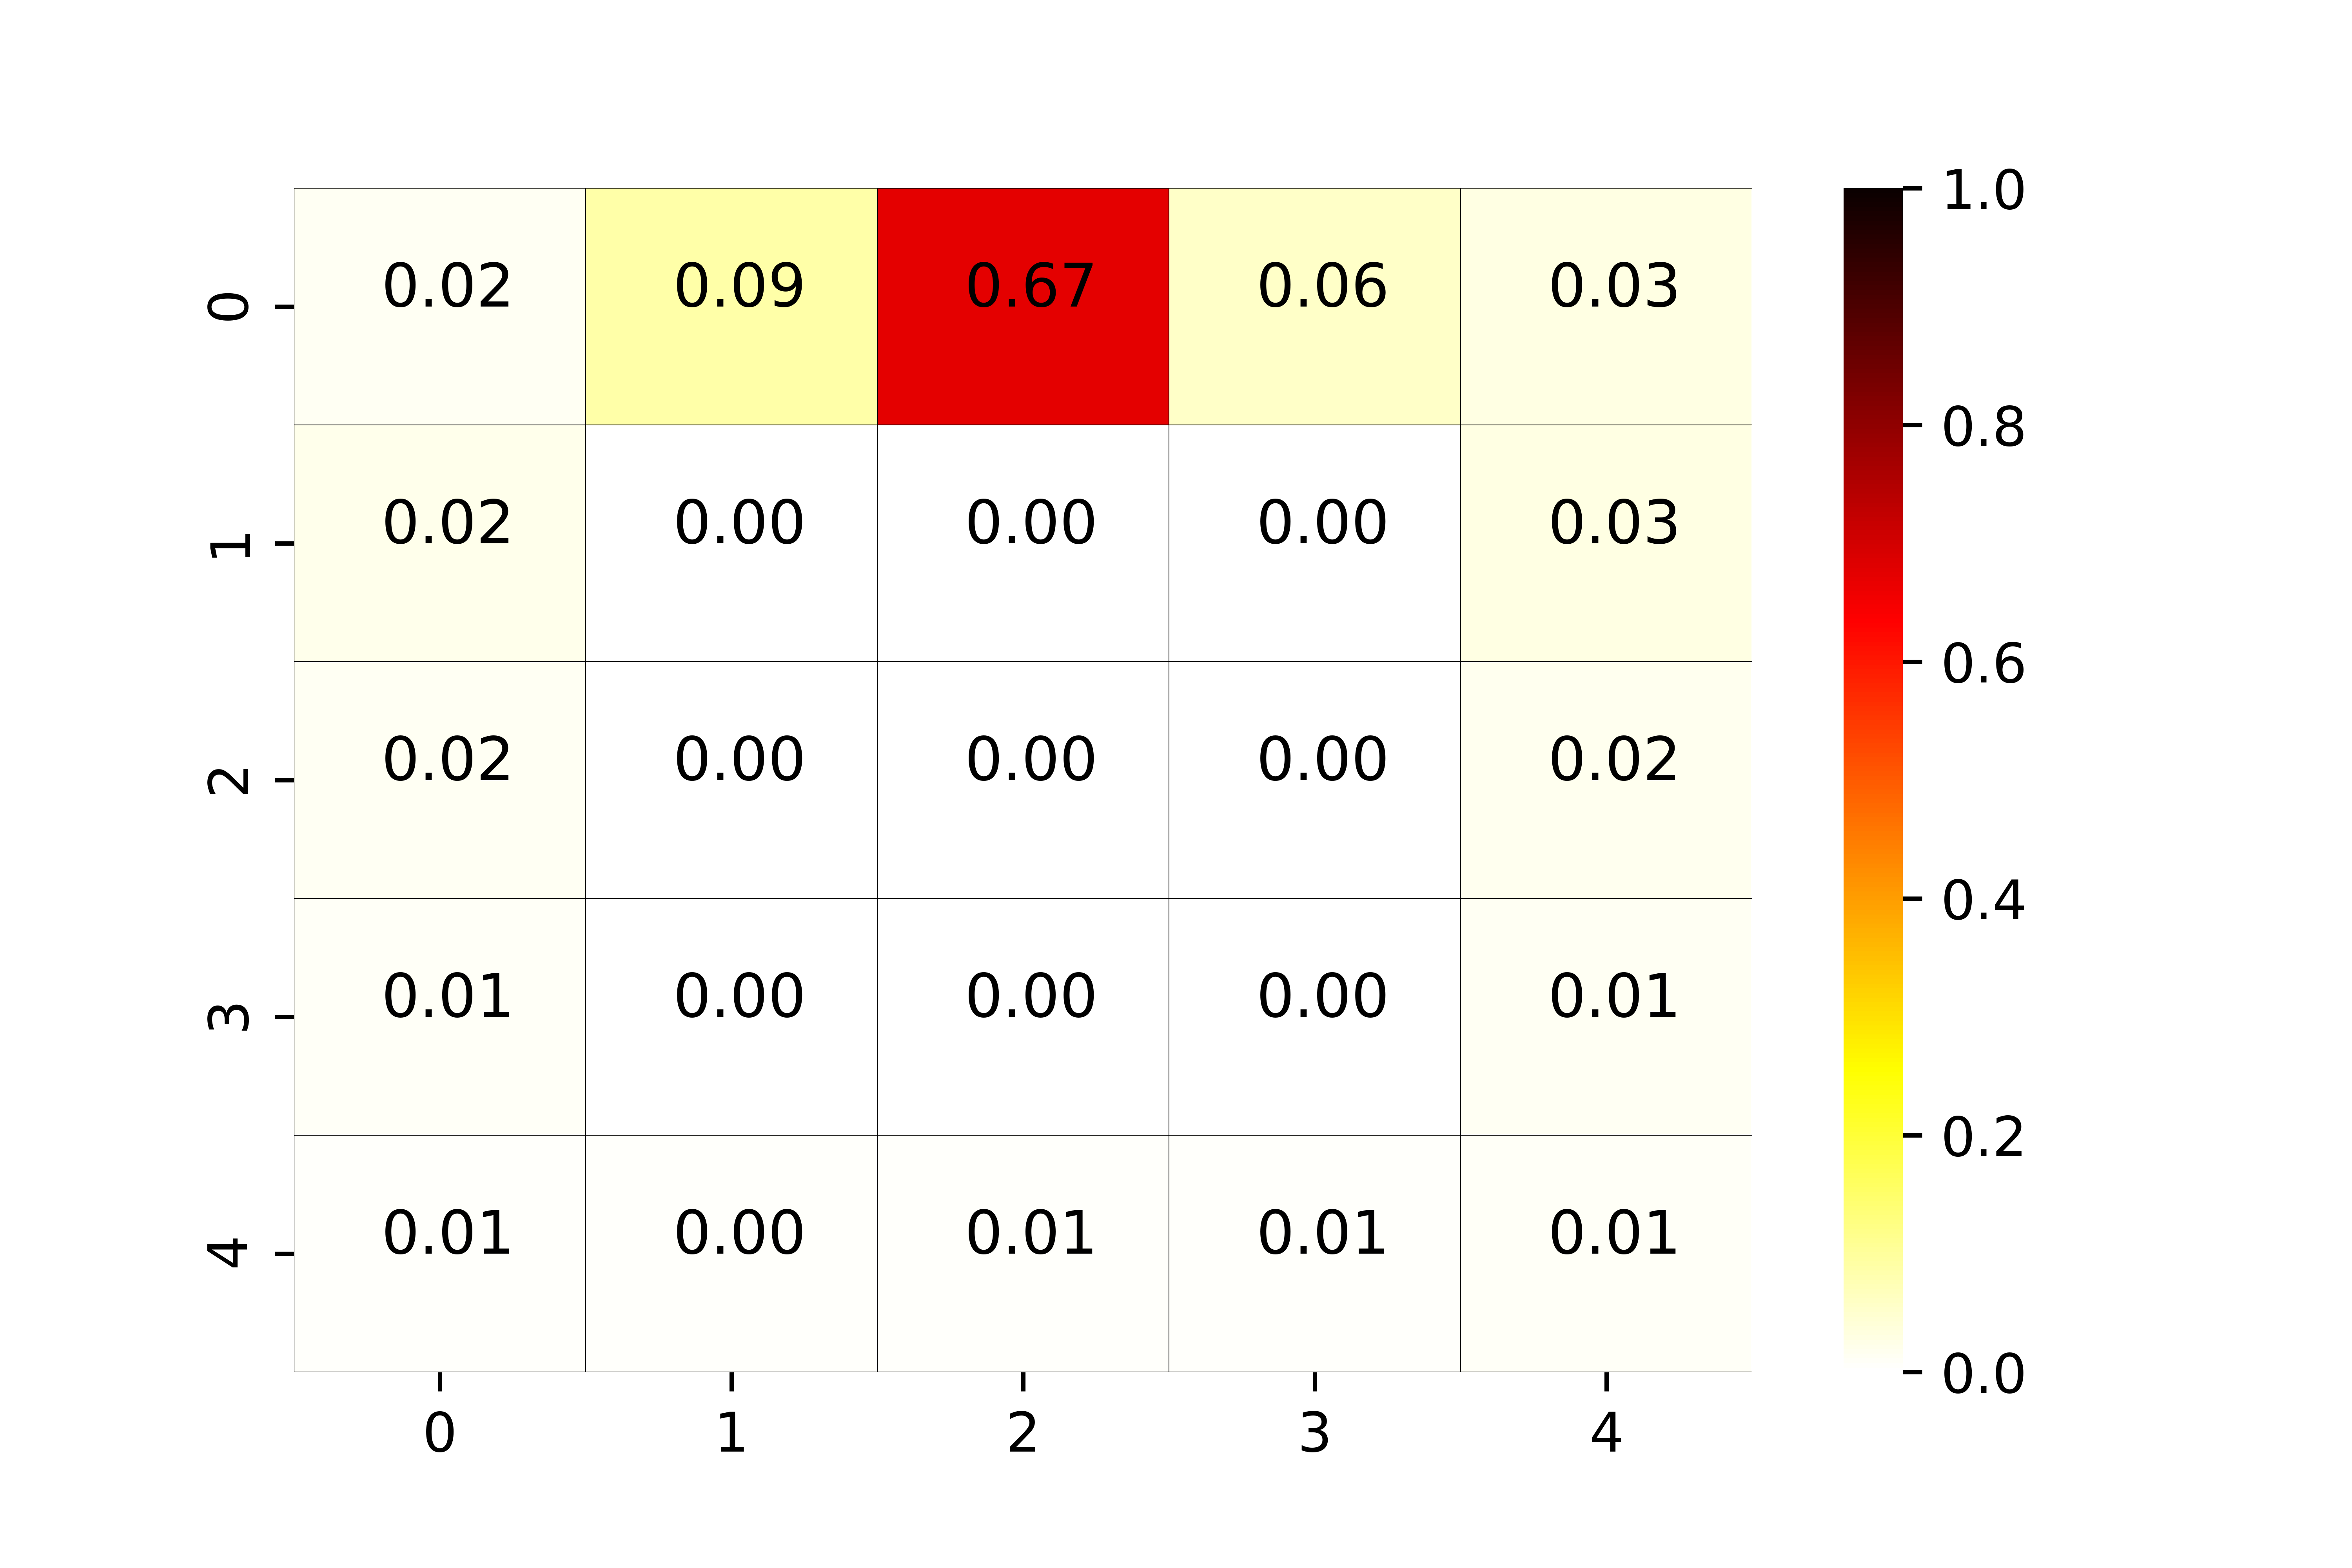
\includegraphics[width=\textwidth]{plots/colormap99.png}
		\caption{Robot Adaptation: abstract state visitation frequencies at the $99$-th (final) iteration of DPO.}
		\label{fig:cm99}
	\end{minipage}
\end{figure}

\begin{figure}[h!]
	\centering
	\begin{minipage}[t]{.48\columnwidth}
		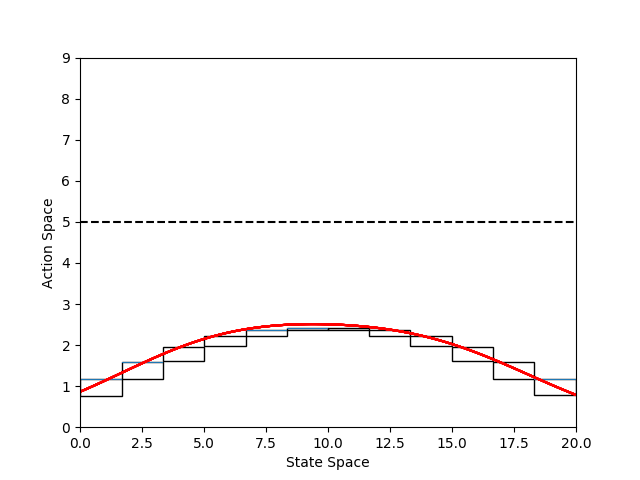
\includegraphics[width=\textwidth]{plots/it0.png}
		\caption{Minigolf: initial policy for DPO.}
		\label{fig:mg0}
	\end{minipage}%
	\hfill
	\begin{minipage}[t]{.48\columnwidth}
		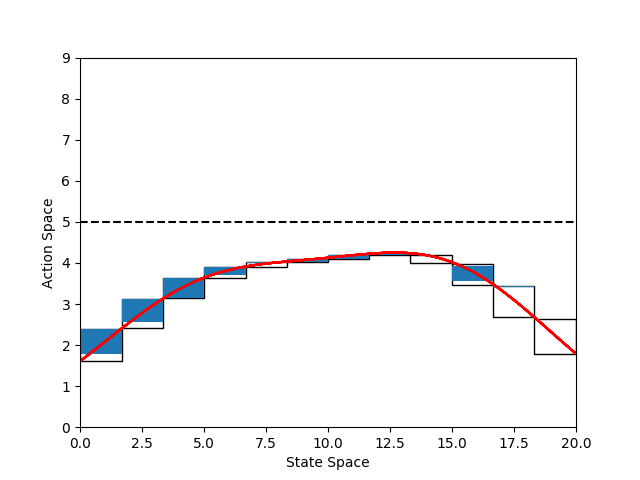
\includegraphics[width=\textwidth]{plots/it33.png}
		\caption{Minigolf: policy after $33$ iterations of DPO.}
		\label{fig:mg33}
	\end{minipage}
\end{figure}
\begin{figure}[h!]
	\centering
	\begin{minipage}[t]{.48\columnwidth}
		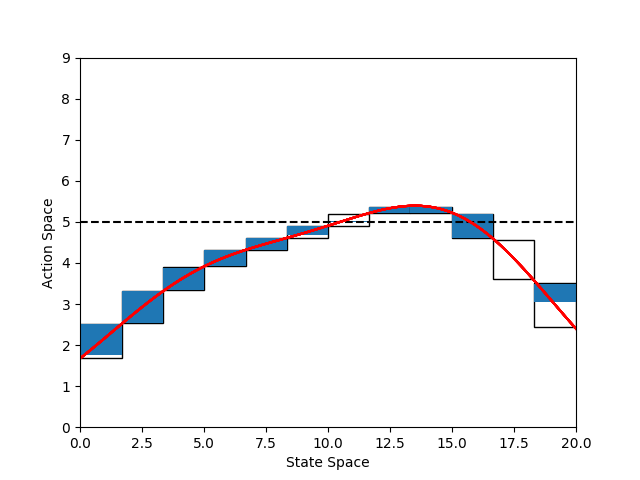
\includegraphics[width=\textwidth]{plots/it66.png}
		\caption{Minigolf: policy after $66$ iterations of DPO.}
		\label{fig:mg66}
	\end{minipage}%
	\hfill
	\begin{minipage}[t]{.48\columnwidth}
		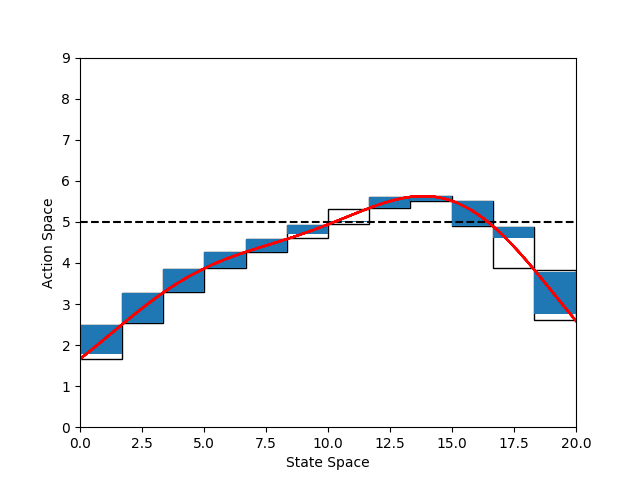
\includegraphics[width=\textwidth]{plots/it99.png}
		\caption{Minigolf: policy after $99$ iterations of DPO.}
		\label{fig:mg99}
	\end{minipage}
\end{figure}
\begin{figure}[h!]
	\centering
	\begin{minipage}[t]{.48\columnwidth}
		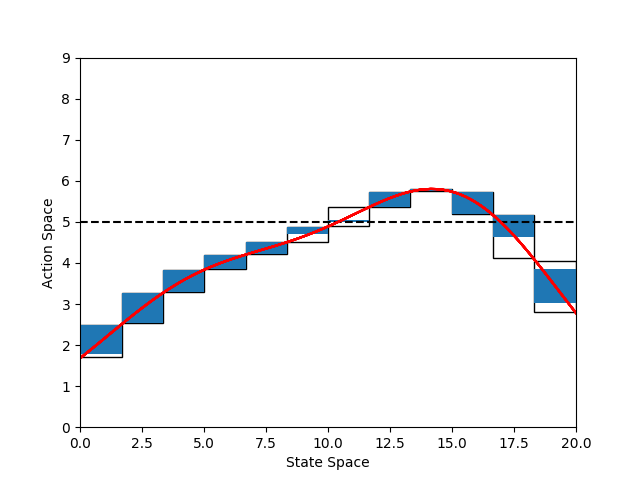
\includegraphics[width=\textwidth]{plots/it199.png}
		\caption{Minigolf: policy after $199$ iterations of DPO.}
		\label{fig:mg199}
	\end{minipage}%
	\hfill
	\begin{minipage}[t]{.48\columnwidth}
		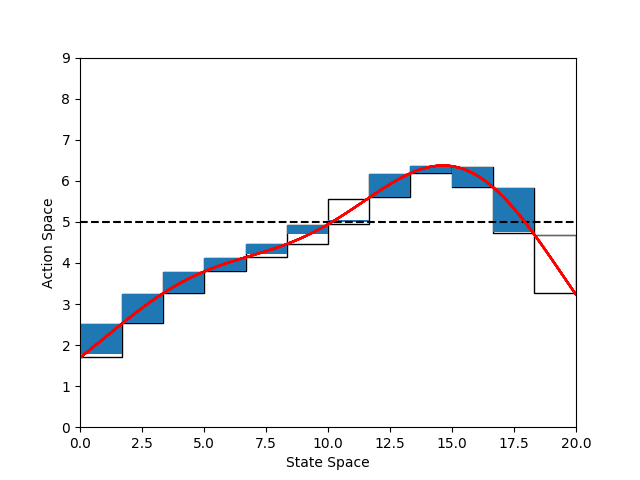
\includegraphics[width=\textwidth]{plots/it299.png}
		\caption{Minigolf: policy after $299$ iterations of DPO.}
		\label{fig:mg299}
	\end{minipage}
\end{figure}
\begin{figure}[h!]
	\centering
	\begin{minipage}[t]{.48\columnwidth}
		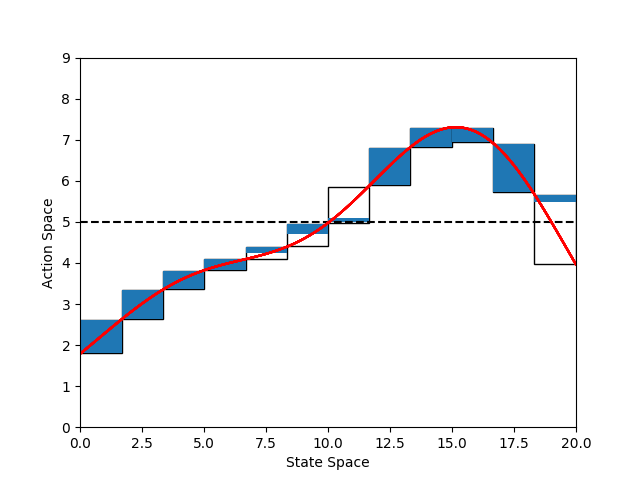
\includegraphics[width=\textwidth]{plots/it399.png}
		\caption{Minigolf: policy after $399$ iterations of DPO.}
		\label{fig:mg399}
	\end{minipage}%
	\hfill
	\begin{minipage}[t]{.48\columnwidth}
		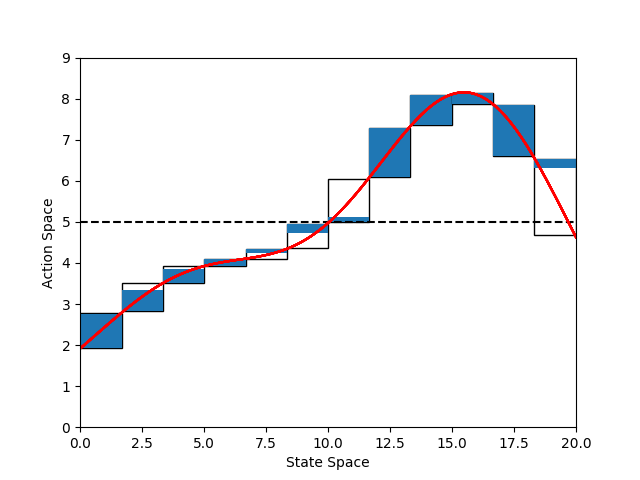
\includegraphics[width=\textwidth]{plots/it499.png}
		\caption{Minigolf: final policy after $499$ iterations of DPO.}
		\label{fig:mg499}
	\end{minipage}
\end{figure}

\clearpage
	
	% ************************************************************
	% Backmatter
	%*************************************************************
	\cleardoublepage\include{FrontBackmatter/AutoParts/Bibliography}
	\appendix
	% \cleardoublepage\part{Appendix}
	\include{Chapters/Code_listings}

\end{document}
% ****************************************************************